\documentclass[11pt]{article}
\usepackage[T1]{fontenc}
\usepackage[utf8]{inputenc}
\usepackage{mathpazo}
\usepackage[margin=1in]{geometry}
\usepackage{amsmath,amssymb,amsthm,mathtools}
\usepackage{microtype}
\usepackage{booktabs,array,enumerate}
\usepackage{tikz}
\usetikzlibrary{arrows.meta}
\usepackage[numbers,sort&compress]{natbib}
\usepackage{xcolor}
\usepackage{hyperref}
\usepackage{bookmark}
\hypersetup{colorlinks=true,linkcolor=blue!40!black,
  citecolor=blue!40!black,urlcolor=blue!40!black,
  pdflang={en},bookmarksdepth=2,
  pdftitle={The joint Dickman law for consecutive integers},
  pdfauthor={OpenAI},
  pdfsubject={Joint Dickman independence in ordinary natural density}}
\urlstyle{same}
\newcommand{\E}{\mathbb E}
\newcommand{\Prob}{\mathbb P}
\newcommand{\ind}{\mathbf 1}
\newcommand{\whZ}{\widehat{\mathbb Z}}
\newcommand{\N}{\mathbb N}
\newcommand{\Z}{\mathbb Z}
\newcommand{\R}{\mathbb R}
\newcommand{\C}{\mathbb C}
\newcommand{\Pplus}{P^+}
\newcommand{\dd}{\,\mathrm d}
\DeclareMathOperator{\supp}{supp}
\DeclareMathOperator{\Var}{Var}
\DeclareMathOperator{\sgn}{sgn}
\newtheorem{theorem}{Theorem}[section]
\newtheorem{proposition}[theorem]{Proposition}
\newtheorem{lemma}[theorem]{Lemma}
\newtheorem{corollary}[theorem]{Corollary}
\theoremstyle{definition}
\newtheorem{definition}[theorem]{Definition}
\theoremstyle{remark}
\newtheorem{remark}[theorem]{Remark}
\numberwithin{equation}{section}
\setlength{\emergencystretch}{2em}
\setcounter{tocdepth}{1}
\allowdisplaybreaks[1]
\input{glyphtounicode}
\pdfgentounicode=1
\pdftrailerid{}
\pdfsuppressptexinfo=15

\title{The joint Dickman law for consecutive integers}
\author{OpenAI}
\date{September 24, 2026}
\begin{document}
\maketitle
\begin{abstract}
Let $P^+(n)$ denote the largest prime factor of $n$. We prove that
$\log P^+(n)/\log n$ and $\log P^+(n+1)/\log n$ are asymptotically
independent in ordinary natural density, with Dickman marginals. This resolves the Erd\H{o}s--Pomerance
joint Dickman conjecture positively and implies that the ordering
$P^+(n)<P^+(n+1)$ has natural density $1/2$.
\end{abstract}
\tableofcontents
\clearpage
\section{Introduction}\label{sec:introduction}

For an integer $n\geq2$, let $\Pplus(n)$ denote its largest prime divisor,
and put $\Pplus(1)=1$.  The Dickman--de Bruijn function $\rho$ is the
continuous function on $[0,\infty)$ determined by
\[
 \rho(u)=1\quad(0\leq u\leq1),\qquad
 u\rho'(u)=-\rho(u-1)\quad(u>1).
\]
The classical theory of smooth
numbers, beginning with Dickman and developed by Ramaswami and
de Bruijn~\cite{Dickman1930,Ramaswami1949,deBruijn1951}, gives
\[
 \frac1X\#\{n\leq X:\Pplus(n)\leq X^a\}
 \longrightarrow \rho(1/a)\qquad(0<a\leq1).
\]
Our result identifies the joint law at two consecutive integers.

\begin{theorem}[Joint Dickman law]\label{thm:main}
For every fixed $a,b\in(0,1)$,
\[
 \lim_{X\to\infty}\frac1X
 \#\{2\leq n\leq X:\Pplus(n)\leq n^a,
                         \ \Pplus(n+1)\leq n^b\}
 =\rho(1/a)\rho(1/b).
\]
Here the limit is taken over all real $X$, with ordinary, unweighted
counting.
\end{theorem}

Thus $\log\Pplus(n)/\log n$ and $\log\Pplus(n+1)/\log n$ have, in natural
density, independent limiting distributions with distribution function
$a\mapsto\rho(1/a)$, continuously extended to $[0,1]$.
Section~\ref{sec:distribution} proves the corresponding law with fixed
thresholds $X^a,X^b$, derives the displayed moving-threshold statement,
and identifies this continuous limiting law.  Inclusion--exclusion using
the fixed-threshold law and its marginals gives the upper-tail independence conjecture of
Erd\H{o}s and Pomerance~\cite[p.~311]{ErdosPomerance1978}.

The comparison conjecture usually attributed to Erd\H{o}s and Tur\'an is
a consequence, rather than a separate main theorem.

\begin{corollary}\label{cor:comparison}
One has
\[
 \lim_{X\to\infty}\frac1X
 \#\{2\leq n\leq X:\Pplus(n)<\Pplus(n+1)\}=\frac12.
\]
The reverse ordering has the same natural density.
\end{corollary}

The limiting marginal is continuous, so its product measure gives zero
mass to the diagonal; symmetry then gives the corollary.  In particular,
no quantitative separation estimate is needed for this deduction.

\subsection{Previous work}

Erd\H{o}s and Pomerance~\cite{ErdosPomerance1978} formulated the joint
independence problem and proved that each ordering has positive lower
natural density.  Their explicit lower bound was $0.0099$.  They also
proved that for every $\varepsilon>0$, some $\delta>0$ makes the number of
integers $n<X$ satisfying
$X^{-\delta}<\Pplus(n)/\Pplus(n+1)<X^\delta$ less than $\varepsilon X$
for all sufficiently large $X$~\cite[Theorem~1]{ErdosPomerance1978}.
The lower-density bound was increased to $0.05544$ by de la Bret\`eche,
Pomerance and Tenenbaum~\cite[Section~3]{BretechePomeranceTenenbaum2005},
and to $0.05866$ by an observation of Fouvry recorded in the same section.
Wang~\cite{Wang2017,Wang2018} obtained $0.1063$ and $0.1356$, and
L\"u and Wang~\cite{LuWang2025} obtained $0.2017$.
Yang's recent preprint~\cite[Theorem~1.4]{Yang2026} gives $0.280$ for both
orderings.  These are bounds on lower natural densities; they do not
assert that a natural density exists.

For the joint law itself,
Ter\"av\"ainen~\cite[Theorem~1.14]{Teravainen2018} proved the predicted
product in logarithmic density.  That is, for fixed $0<a,b<1$, the
indicator in Theorem~\ref{thm:main}, averaged with weight $1/n$ and
normalization $1/\log X$, tends to $\rho(1/a)\rho(1/b)$.
His Theorem~1.16 gives logarithmic density $1/2$ for the ordering, while
Theorem~1.19 proves positive lower natural density for every nondegenerate
rectangle of normalized largest-prime-factor values inside $(0,1)^2$.
Tao and Ter\"av\"ainen~\cite[Remark~3.3, equation~(50)]{TaoTeravainen2019}
then obtained the joint product law for ordinary averages outside an
exceptional set of scales of logarithmic density zero; their
Corollary~1.16 gives the corresponding ordering result.
Wang~\cite{Wang2021Conditional} proved the ordinary joint law under the
Elliott--Halberstam conjecture for friable integers.  Jiang, L\"u and
Wang~\cite{JiangLuWang2022} established averaged-over-shift forms of the
conjectures, a different conclusion from a result at the fixed shift one.

The more recent work of Tao and
Ter\"av\"ainen~\cite[Theorem~1.8]{TaoTeravainen2026Quantitative} gives
a quantitative joint law outside an exceptional set of scales, with
uniformity in the smoothness parameters and a power saving in $\log X$.
Theorem~\ref{thm:main} concerns fixed parameters and has no exceptional
scales; it does not assert their quantitative error term or their
uniformity for growing parameters.  Relative to the results just
described, the distinction is therefore the unconditional ordinary limit
at every sufficiently large scale, not a new marginal distribution or
a logarithmically averaged independence statement.

\subsection{Method and organization}

We first replace the largest prime factor by finitely many prime counts.
For a fixed integer $J\ge2$, divide the primes in $(x^{1/J},x]$ into
bins $\mathcal B_{k,x}=(x^{k/J},x^{(k+1)/J}]$, $1\le k<J$.  If
$\Omega_E(n)$ counts prime factors in $E$ with multiplicity, a choice of
unit complex numbers $\zeta_k$ defines the bin character
\[
 f_x(n)=\prod_{k=1}^{J-1}\zeta_k^{\Omega_{\mathcal B_{k,x}}(n)}.
\]
Let $g_x$ be defined by a second arbitrary phase vector, and
let $F_x=f_x-\mu$, where $\mu$ is the limiting mean of $f_x$.  Finite
Fourier inversion reduces the joint law to the mixed decorrelation
\[
 \frac1x\sum_{n<x}\overline{g_x(n)}F_x(n+1)\longrightarrow0.
\]
Here $x$ runs through integer scales.
The two phase vectors may differ.  This freedom gives independence of
the two count vectors.

Two properties of these functions connect the beginning and end of the
proof.  First, every fixed positive integer multiplier has all its prime factors
below the bins once $x$ is large.  Thus $F_x(un)=F_x(n)$ and
$g_x(un)=g_x(n)$ for each fixed $u$.  Second, $F_x$ has cancellation in
averages over growing intervals that remain short relative to the original
scale.  Let $B$ be the auxiliary parameter and let $T=T(B)\to\infty$ be
the growing shift scale.  If $P_B$ is a finite set of primes with
$\min P_B\to\infty$, define
\[
 G_{B,v}(n)=\prod_{\substack{p\in P_B\\p\mid n}}
                 \frac{1+p^{-v/B}}2,\qquad v\ge0.
\]
For any interval $I_B$ of $L_B\to\infty$ consecutive integer shifts,
and fixed $0<s_0<s_1$, positive integer $D$, residue $r\pmod D$, and $v\ge0$,
Section~\ref{sec:labels} proves
\[
 \lim_{B\to\infty}\limsup_{x\to\infty}
 \frac1{Tx}\sum_{s_0Tx\le n\le s_1Tx}
 \left|\frac1{L_B}
   \sum_{\substack{i\in I_B\\i\equiv r\pmod D}}
     F_x(n+i)G_{B,v}(n+i)\right|^2=0.
\]
At fixed $B$ the shift interval is short relative to $x$, while the base
points have size $Tx$.  This is the scale produced by the divisor
substitution below.

The centered function $F_x$ is not multiplicative.  On the relevant ranges
$n=O_B(x)$, the bin counts take values in a fixed finite set.  This permits
interpolation by a fixed finite family of real,
nonnegative multiplicative functions.  After resolving the residue
condition by Dirichlet characters, the real short-interval theorem of
Matom\"aki and Radziwi\l\l~\cite[Theorem~1]{MatomakiRadziwill2016} compares
the principal components with long means whose centered combination
vanishes.  The complex theorem of Matom\"aki, Radziwi\l\l\ and
Tao~\cite[Theorem~A.1, corrected version]{MatomakiRadziwillTao2015}
controls the nonprincipal twists.  The rest of the proof must reduce
the mixed correlation to this particular cancellation statement.

Suppose, then, that the mixed correlation stays nonzero along a sequence
of scales.  The profinite integers $\widehat{\mathbb Z}$ encode compatible
residue classes modulo all positive integers and carry Haar probability
measure.  Passing to a subsequence gives a bounded profile $W(t,w)$ on
$(0,\infty)\times\widehat{\mathbb Z}$.  Its integral against each fixed
compactly supported continuous test $\Phi(t,w)$ is the subsequential limit
of the mixed averages weighted by $\Phi(n/x,n)$, with $n$ in the second
argument viewed through its residues.  A fixed nonnegative compactly
supported smooth cutoff $\phi$ can be chosen so that
$\int\phi(t)W(t,w)\,dt\,dw\ne0$, where $dt$ is Lebesgue measure and $dw$
is Haar measure.

For an integer $n$, the amplifier defines $D_B(n)$ as a nonnegative
weighted count of factorizations $n=am$ and $n+1=cl_a$, restricted by
$e^B<c<e^{2B}$ and $Tc<a<2Tc$.  At fixed $B$ its coefficient list is
finite, and the same formula defines a function on $\widehat{\mathbb Z}$
depending only on residues at primes above a cutoff tending to infinity.
The construction gives $D_B$ Haar mean at least $d_0>0$ for large $B$ and
bounded $L^2$ norm.  To prove these bounds, the argument passes to a
comparison model in which each site prime is assigned by an independent
fair coin to the coefficient divisor or the remaining factor.  The first
and second moments are analyzed through one split and two conditionally
independent splits of the same site prime sets.  For each fixed $B$,
$\Phi(t,w)=\phi(t)D_B(w)$ is an allowed profile test, so along the selected
subsequence
\[
 \lim_{x\to\infty}\frac1x\sum_{n\ge1}
   \phi(n/x)\overline{g_x(n)}F_x(n+1)D_B(n)
 =\int\phi(t)W(t,w)D_B(w)\,dt\,dw.
\]
Independence from every fixed residue coordinate and $L^2$ approximation
of $\phi W$ show that the right-hand side has absolute value bounded away
from zero as $B\to\infty$.

For fixed $B$ and large $x$, writing $n=am$ in this weighted average
replaces $g_x(n)$ by $g_x(m)$.
For each fixed pair $(c,m)$, the remaining terms form a sum over
$a$ satisfying $c\mid am+1$, with nonnegative divisor and smooth weights
multiplying $F_x(am+1)$.  Cauchy--Schwarz in $(c,m)$ removes the
unit-modulus factor $g_x(m)$ and squares this inner sum.  The resulting
normalized quadratic energy has a positive lower bound, while its
equal-coefficient diagonal tends to zero in the same iterated limit.  A positive contribution
therefore remains from distinct indices $a,b$.
Section~\ref{sec:amplification} proves these moment and energy claims.

For such a pair, $c$ divides both $am+1$ and $bm+1$.  Thus $m$ is a unit
modulo $c$ and $a-b=jc$, with $0<|j|<T$ by the coefficient windows.  Writing
$l_a=(am+1)/c$ and $l_b=(bm+1)/c$, the exact substitution
\[
 n'=b l_a,\qquad n'+j=a l_b
\]
turns the label product into $\overline{F_x(n')}F_x(n'+j)$ by invariance
under the fixed multipliers $a,b,c$.  The new endpoints have size $Tx$.
The off-diagonal energy is therefore a weighted graph of ordinary additive
shifts.  Its edge weights depend on endpoint prime sets and on additional
residue data from each divisor representation.

Group the new endpoints into blocks $N+i$, $1\le i\le M$, with
$M=\lceil C_6T\rceil$ for a fixed large $C_6$, and put $s=N/(Tx)$.
Section~\ref{sec:graph} couples the actual auxiliary-prime divisibility
sets at these positions to independent model sets $S_i$, each
formed by including every auxiliary prime $p$ independently with probability $1/p$, and averages
the extra residue weight of each representation.  This compares the
arithmetic graph with an endpoint kernel
$\mathcal L_{ik}(S_i,S_k;s)$ in expected cut norm.  Here cut norm is the
largest absolute normalized pairing with two real vectors bounded by one,
chosen after the matrix is known.  Section~\ref{sec:moments} controls
representation multiplicity and provides the averaged second-moment
bounds needed for sampling.

The aim is now to replace this endpoint kernel by products of functions of
its two endpoints.  For an endpoint type $S$, let $b$ be the product
obtained by retaining each prime independently
with probability $1/2$.  The features used in the comparison are
\[
 V_l(S)=\frac1{|I_l|}
   \Prob_{\rm split}\!\left(\frac{\log b}{B}\in I_l\,\middle|\,S\right),
\]
where the $I_l$ form a fixed coarse partition of a compact logarithmic
interval, chosen for a desired accuracy.  The channel estimates in Section~\ref{sec:channels} show that
fair splitting suppresses residue dependence and makes logarithmic
outputs uniformly approximable on this partition.  Fourier detection of
$a-b=jc$ then lets Section~\ref{sec:kernel} apply arithmetic estimates to
the coefficient $c$ and these channel estimates to the endpoints.  The
resulting comparison has the form
\[
 \sum_l c_{l,B}(j,s)V_l(S_i)V_l(S_k),\qquad j=k-i,
\]
where $i,k$ are the endpoint positions.  The scalar coefficients separate
an arithmetic factor in $|j|$ from a smooth factor in the normalized lag
$|j|/T$ and the common block origin $s$.  The number of features is fixed,
while their values and the coefficients may depend on $B$.

The feature comparison first holds after integration against separate
functions of the two independent endpoint sets.  The actual labels need
not have this single-site form, and an optimizing test can depend on the
whole configuration.  Section~\ref{sec:sampling} upgrades the comparison
to expected cut norm by approximating an optimizing cut with a small sample
of columns.  Finally,
polynomial approximation of each log-window indicator expresses $V_l$,
up to a small mean-square error, as a fixed finite combination of
\[
 \E_{\rm split}\!\left[e^{-v\log b/B}\mid S\right]
       =\prod_{p\in S}\frac{1+p^{-v/B}}2.
\]
At an integer endpoint these are exactly $G_{B,v}$.  The arithmetic lag
factor is approximated in mean over lags by a fixed periodic function.
For a fixed small $\delta>0$ chosen for the desired accuracy, subdivide each
position block into a fixed number of intervals whose lengths grow with
$T$ and are at most $\delta T$.  Within each interval pair, the normalized
lag varies by at most $2\delta$.  Approximating the smooth lag factor there
and resolving the periodic factor into fixed residue classes turns the
feature energy, up to a controlled error, into products of the weighted
short averages already controlled in Section~\ref{sec:labels}.  Their vanishing
contradicts the positive energy.  Sections~\ref{sec:conclusion}
and~\ref{sec:distribution} complete this argument and the passage from bin
events to the joint law.

The divisor amplification and graph comparison have close antecedents in
Tao's logarithmic correlation argument~\cite{Tao2016LogChowla}, the
prime-divisibility graphs of Helfgott and
Radziwi\l\l~\cite{HelfgottRadziwill2021}, Pilatte's product-of-primes
amplification~\cite{Pilatte2023}, and the mixed-function decoupling of
Tao and Ter\"av\"ainen~\cite[Section~3.1]{TaoTeravainen2026Quantitative}.
The present rough-divisor graph and its endpoint comparison are proved
locally.  The sampling argument likewise builds on the cut-based methods
of Frieze and Kannan~\cite{FriezeKannan1999}, Alon, Fernandez de la Vega,
Kannan and Karpinski~\cite[Lemma~3]{AlonEtAl2003Sampling}, and Borgs,
Chayes, Lov\'asz, S\'os and
Vesztergombi~\cite[Theorem~4.6]{BorgsEtAl2008}.  Because the kernels here
vary with $B$ and can be large, the proof establishes the moment bounds
needed before applying bounded-differences concentration~\cite{McDiarmid1989}.

The arithmetic estimates are developed in Section~\ref{sec:arithmetic}
using Selberg--Delange theory, character estimates and upper-bound sieves
in the forms recorded by Granville and
Koukoulopoulos~\cite{GranvilleKoukoulopoulos2019},
Koukoulopoulos~\cite{Koukoulopoulos2019}, and
Ford~\cite{FordSieve2023,FordZeta2022}.  The minor-arc input in
Section~\ref{sec:kernel} is the exponential-sum estimate of Montgomery and
Vaughan~\cite{MontgomeryVaughan1977}.  Throughout the proof, the original
scale $x$ tends to infinity before the auxiliary scale $B$.  Bin data,
feature degrees, residue moduli and divisor multipliers are fixed in that
inner limit.  The contradiction applies to a subsequence of every possible
bad sequence of original scales, and hence yields the full ordinary limit.

\section{Large-prime labels and their short averages}\label{sec:labels}

We encode the large prime factors by two independently chosen multiplicative
labels.  Their one-variable distributions have limits independent of fixed
residue conditions.  We establish those limits and the weighted short-average
estimate needed to prove that the two labels decorrelate at consecutive
integers.  In the short-average estimate the original counting scale $x$ tends to
infinity before the auxiliary parameter $B$ does.
The scale $x>1$ is real unless a statement explicitly restricts it to integers.

\subsection{Labels and their one-variable distributions}

Fix an integer $J\geq2$.  For $1\leq k<J$ put
\begin{equation}\label{eq:labels-bins}
 \mathcal B_{k,x}=(x^{k/J},x^{(k+1)/J}].
\end{equation}
If $E$ is a set of primes, $\Omega_E(n)$ denotes the number of prime factors
of $n$ belonging to $E$, counted with multiplicity.  Fix complex numbers
$\zeta_1,\ldots,\zeta_{J-1}$ and $\xi_1,\ldots,\xi_{J-1}$ of absolute
value one, independent of $x$, with no relation required between the two
vectors.  Define the completely multiplicative function $f_x$ by
\begin{equation}\label{eq:labels-function}
 f_x(p)=
 \begin{cases}
  \zeta_k,&p\in\mathcal B_{k,x},\quad 1\leq k<J,\\
  1,&p\notin\bigcup_{1\leq k<J}\mathcal B_{k,x}.
 \end{cases}
 \qquad
 f_x(n)=\prod_{k=1}^{J-1}\zeta_k^{\Omega_{\mathcal B_{k,x}}(n)}.
\end{equation}
Define the completely multiplicative label associated with $(\xi_k)$ by
\begin{equation}\label{eq:labels-second-function}
 g_x(n)=\prod_{k=1}^{J-1}\xi_k^{\Omega_{\mathcal B_{k,x}}(n)}.
\end{equation}
Both labels have absolute value one.
For every fixed $C>0$, every integer $n\leq Cx$ has at most $J$ prime
factors in the union of the bins, once $x$ is sufficiently large in terms
of $C,J$.  Indeed, $J+1$ such factors would have product exceeding
$x^{1+1/J}>Cx$.

\begin{lemma}[One-variable distribution]\label{lem:labels-marginal}
For every fixed $0<\alpha<\beta<\infty$, positive integer $q$, and residue
class $a\pmod q$, the distribution of
\[
 \bigl(\Omega_{\mathcal B_{k,x}}(n)\bigr)_{1\leq k<J}
\]
among the integers $\alpha x<n\leq\beta x$, $n\equiv a\pmod q$,
normalized to have mass one, converges as $x\to\infty$.  Its limit depends
only on $J$, and not on $\alpha,\beta,q,a$.

Consequently there is a number $\mu=\mu(J,\zeta_1,\ldots,\zeta_{J-1})$
with $|\mu|\leq1$ such that
\begin{equation}\label{eq:labels-marginal-mean}
 \lim_{x\to\infty}
 \frac{q}{(\beta-\alpha)x}
 \sum_{\substack{\alpha x<n\leq\beta x\\n\equiv a\pmod q}}f_x(n)
 =\mu.
\end{equation}
The same assertion holds for $g_x$, with a mean $\mu_g$ depending only
on $J$ and the vector $(\xi_k)_{k=1}^{J-1}$.
Write
\begin{equation}\label{eq:labels-centered}
 F_x(n)=f_x(n)-\mu.
\end{equation}
Then $|F_x(n)|\leq2$, and for every fixed positive integer $u$,
\begin{equation}\label{eq:labels-multiplier}
 F_x(un)=F_x(n),\qquad g_x(un)=g_x(n)\qquad(n\geq1)
\end{equation}
for all sufficiently large $x$ in terms of $u,J$.
\end{lemma}

\begin{proof}
We prove convergence by computing all mixed factorial moments of the
bin counts.  We first record the elementary prime estimates used in this
calculation.  Put $\vartheta(z)=\sum_{p\le z}\log p$.  For $z\ge2$ we have
\begin{equation}\label{eq:distribution-prime-estimates}
 \vartheta(z)\ll z,\qquad
 \pi(z)\ll\frac z{\log z},\qquad
 \sum_{p\le z}\frac{\log p}{p}=\log z+O(1).
\end{equation}
Indeed, the primes in $(m,2m]$ divide $\binom{2m}{m}$, giving
$\vartheta(2m)-\vartheta(m)\ll m$.  Dyadic summation proves the first
estimate, and separating the primes at $\sqrt z$ proves the second.
Moreover,
\[
 \sum_{p^\nu\le z}\log p
 =\sum_{1\le\nu\le\log_2z}\vartheta(z^{1/\nu})\ll z,
\]
because the terms with $\nu\ge2$ are $O(\sqrt z\log z)$.
Expanding $\log n$ over prime powers now gives
\[
 \sum_{n\le z}\log n
 =\sum_{p^\nu\le z}\log p\,\lfloor z/p^\nu\rfloor
 =z\sum_{p\le z}\frac{\log p}{p}+O(z).
\]
The floor errors use the preceding prime-power bound, and the terms
with $\nu\ge2$ use
$\sum_p\sum_{\nu\ge2}(\log p)/p^\nu<\infty$.
Integral comparison on the left proves the third estimate in
\eqref{eq:distribution-prime-estimates}.  Partial summation yields
\begin{equation}\label{eq:distribution-prime-measure}
 \sum_{x^s<p\le x^t}\frac1p\longrightarrow\log(t/s)
 \qquad(0<s<t\ \text{fixed}),
\end{equation}
as well as $\sum_{p\le z}1/p=\log\log z+O(1)$.

The number of integers $n\leq\beta x$ divisible by $p^2$ for some
prime $p>x^{1/J}$ is at most
\[
 \beta x\sum_{p>x^{1/J}}\frac1{p^2}+O_\beta(\sqrt x)=o(x).
\]
This remains negligible relative to the size of any one fixed progression
in the lemma.  We may therefore replace multiplicity counts by counts of
distinct primes.

For the mixed factorial moments of these distinct-prime counts, write
$(b)_r=b(b-1)\cdots(b-r+1)$ and $(b)_0=1$.
Fix nonnegative integers $r_1,\ldots,r_{J-1}$, and let
$r=r_1+\cdots+r_{J-1}$.  The case $r=0$ is immediate.  For $r>0$, a term
in the factorial-moment expansion selects, in order, $r_k$ distinct
primes from bin $k$, for each $k$.  Denote their product by $d$; only
$d\leq\beta x$ can contribute.  The number of such selections is
$O_{J,\beta,r}(x/\log x)$.  To see this, fix every selected prime except
one, and write $d_1$ for their product.  If the last prime has any
admissible choice, its upper bound $\beta x/d_1$ exceeds $x^{1/J}$.
The prime-counting upper bound therefore gives at most
\[
 O_{J,\beta}\!\left(\frac{x}{d_1\log x}\right)
\]
choices.  Summing this bound over the other primes costs a bounded product
of reciprocal prime sums over the bins.  We may drop distinctness and
product restrictions when taking this upper bound.

For sufficiently large $x$, every selected prime is coprime to $q$.
The Chinese remainder theorem then gives
\[
 \#\{\alpha x<n\leq\beta x:n\equiv a\pmod q,\ d\mid n\}
 =\frac{(\beta-\alpha)x}{qd}+O(1).
\]
The sum of the errors over all selections is $o(x)$.  After normalization,
the factorial moment is consequently the reciprocal sum over the
selections with $d\leq\beta x$, up to $o(1)$.

In the variable $v=\log p/\log x$, \eqref{eq:distribution-prime-measure}
says that the reciprocal prime measure on bin $k$ converges to $dv/v$
on $(k/J,(k+1)/J]$.  The product restriction is
\[
 \sum_{\text{selected primes}}v\leq1+\frac{\log\beta}{\log x}.
\]
The limiting product measure is absolutely continuous, so the boundary
$\sum v=1$ has measure zero.  Repeated selections do not change the limit:
their reciprocal contribution is bounded by a constant times
$\sum_{p>x^{1/J}}p^{-2}=o(1)$.  Returning from distinct-prime counts to
multiplicity counts also costs $o(1)$ in the normalized moment, because
the exceptional set has size $o(x)$ and the counts are bounded.

List the selected bin indices as $k_1,\ldots,k_r$, with $r_k$
occurrences of $k$.  We have proved the explicit limit
\begin{equation}\label{eq:labels-factorial-limit}
\begin{aligned}
 &\lim_{x\to\infty}\frac{q}{(\beta-\alpha)x}
 \sum_{\substack{\alpha x<n\leq\beta x\\n\equiv a\pmod q}}
       \prod_{k=1}^{J-1}
          \bigl(\Omega_{\mathcal B_{k,x}}(n)\bigr)_{r_k}\\
 &\qquad =
 \int_{\substack{v_i\in(k_i/J,(k_i+1)/J]\ (1\le i\le r)\\
                  v_1+\cdots+v_r\le1}}
       \prod_{i=1}^r\frac{dv_i}{v_i}.
\end{aligned}
\end{equation}
For $r=0$, both sides are one.  The right-hand side depends only on
$J$ and the multi-index $(r_k)$.  All count vectors lie in a fixed
finite set, and mixed factorial polynomials span the functions on that
set.  The asserted distributional convergence follows.

Taking the expectation of the function
$(b_k)\mapsto\prod_k\zeta_k^{b_k}$ gives \eqref{eq:labels-marginal-mean}; using the
vector $(\xi_k)$ gives the mean $\mu_g$.  Finally, if every prime factor
of $u$ is at most $x^{1/J}$, then $f_x(u)=g_x(u)=1$.
Complete multiplicativity of $f_x$ and $g_x$ proves
\eqref{eq:labels-multiplier}.
\end{proof}

The centered function $F_x$ is not asserted to be multiplicative.
Its eventual invariance under each fixed multiplier is the exact property
in \eqref{eq:labels-multiplier} that will be used below.

The same distributional limit holds for averages over $1\leq n\leq x$.
Indeed, apply the lemma to any fixed function of the count vector on
$\alpha x<n\leq x$, then let $\alpha\downarrow0$; that function is
bounded on the finite set of possible vectors, so the omitted interval
has normalized contribution $O(\alpha)$.  In particular,
the limit in \eqref{eq:labels-factorial-limit} is unchanged when its
normalized progression sum is replaced by
$x^{-1}\sum_{1\le n\le x}\prod_k(\Omega_{\mathcal B_{k,x}}(n))_{r_k}$.
This gives \eqref{eq:labels-marginal-mean} on the initial segment as
well.  A fixed shift of the integer argument changes only a bounded
number of terms after nonpositive arguments are omitted, so the label
means have the same limits after such a shift.

\subsection{The mixed correlation and its short-average input}

The joint law will follow by finite Fourier inversion from the following
statement for the two independently chosen phase vectors.  The factor
$F_x(n+1)$ is centered, while $g_x(n)$ has absolute value one.

\begin{proposition}[Mixed decorrelation]\label{prop:mixed}
For every fixed integer $J\geq2$ and every pair of fixed phase vectors
$(\zeta_k)_{k=1}^{J-1}$ and $(\xi_k)_{k=1}^{J-1}$ of absolute value one,
the corresponding labels satisfy
\begin{equation}\label{eq:mixed}
 \lim_{x\to\infty}\frac1x\sum_{1\leq n<x}
                   \overline{g_x(n)}F_x(n+1)=0,
\end{equation}
where $F_x=f_x-\mu$ and the limit is through all integer scales.
\end{proposition}

After establishing the short-average input below, we will suppose that
the average in \eqref{eq:mixed} stays a fixed positive distance from zero
along a sequence and derive a contradiction.  The input is used in
Section~\ref{sec:conclusion} at the final step of the proof.

For each auxiliary parameter $B$, let $P_B$ be a finite set of primes,
and suppose that $\min P_B\to\infty$ as $B\to\infty$.  An empty set
may be allowed by interpreting its minimum as $+\infty$ and its
product as one.  For a fixed real
$v\geq0$, define
\begin{equation}\label{eq:labels-G}
 G_{B,v}(m)=\prod_{\substack{p\mid m\\p\in P_B}}
                   \left(\frac12+\frac12p^{-v/B}\right).
\end{equation}
This is a real, nonnegative, 1-bounded multiplicative function.  For
fixed $B$ it is periodic, with period dividing $\prod_{p\in P_B}p$.
To see its fair-split meaning, put
$S_B(m)=\{p\in P_B:p\mid m\}$ and form a random product $b$ by
including each prime of $S_B(m)$ independently with probability $1/2$.
The empty product is one.  Independence gives
\[
 G_{B,v}(m)
 =\mathbb E_{\mathrm{split}}\!\left[\exp\!\left(-\frac{v\log b}{B}\right)\right].
\]
These are the fair-split averages used to approximate the endpoint
features in Section~\ref{sec:conclusion}.

\begin{lemma}[Weighted short averages of the centered labels]
\label{lem:labels-short}
Let $T=T(B)\to\infty$, let $L_B$ be positive integers tending to
infinity, and let $a_B$ be any integer for each $B$.  Fix
$0<s_0<s_1<\infty$, a positive integer $D$, a residue $r\pmod D$,
and $v\geq0$.  Then
\begin{equation}\label{eq:labels-short}
 \lim_{B\to\infty}\limsup_{x\to\infty}
 \frac1{Tx}\sum_{s_0Tx\leq n\leq s_1Tx}
 \left|
   \frac1{L_B}\sum_{i=a_B+1}^{a_B+L_B}
     \ind_{i\equiv r\ (D)}F_x(n+i)G_{B,v}(n+i)
 \right|^2=0.
\end{equation}
For each fixed $B$ all the arguments of the arithmetic functions are
positive once $x$ is sufficiently large.  The same conclusion holds
if the inner upper limit is taken along any sequence $x\to\infty$.
\end{lemma}

The proof interpolates the centered function of the finitely many bin
counts by real, nonnegative multiplicative functions.  Once the residue of
the origin $n$ is fixed, the congruence on $i$ becomes a fixed residue
condition on the argument $m=n+i$.  Resolving that condition by Dirichlet
characters produces two different tasks.
For the principal character, short averages must be compared with long
means whose centered linear combination vanishes.  For a nonprincipal
character, the short averages themselves must be small.  We record the two
published inputs for these tasks and prove the required distance estimate
before returning to the weighted lemma.

\subsection{The short-interval inputs}

For a bounded arithmetic function $g$ and $H>0$, set
\[
 \mathcal A_Hg(z)=\frac1H\sum_{z<n\leq z+H}g(n),
 \qquad
 \mathcal L_Xg=\frac1X\sum_{X<n\leq2X}g(n).
\]
For a 1-bounded multiplicative function $g$, define
\begin{equation}\label{eq:labels-distance}
 \mathbb D(g,n^{it};X)^2
 =\sum_{p\leq X}\frac{1-\operatorname{Re}(g(p)p^{-it})}{p},
 \qquad
 M(g;X)=\inf_{|t|\leq X}\mathbb D(g,n^{it};X)^2.
\end{equation}

We use the following two forms of the short-interval theorems.  Their
uniformity in the multiplicative function is part of the statements.

\begin{theorem}[Real short-interval comparison]
\label{thm:labels-real-MR}
There is a function $r(H)$ tending to zero as $H\to\infty$ such that,
for every real multiplicative function $g:\N\to[-1,1]$ and
$2\leq H\leq X$,
\begin{equation}\label{eq:labels-real-MR}
 \frac1X\int_X^{2X}
   |\mathcal A_Hg(z)-\mathcal L_Xg|^2\,dz\leq r(H).
\end{equation}
\end{theorem}

This is a consequence of the uniform exceptional-set estimate in
\cite[Theorem~1]{MatomakiRadziwill2016}, using boundedness to pass to
mean square.  The terms in that estimate depending on $X$ can be
absorbed into $r(H)$ because $X\geq H$.

\begin{theorem}[Complex short averages]
\label{thm:labels-complex-MRT}
For every multiplicative function $g:\N\to\C$ with $|g|\leq1$ and
$X\geq H\geq10$,
\begin{equation}\label{eq:labels-complex-quantitative}
 \frac1X\int_X^{2X}|\mathcal A_Hg(z)|^2\,dz
 \ll (1+M(g;X))e^{-M(g;X)}
       +\left(\frac{\log\log H}{\log H}\right)^2
       +(\log X)^{-1/50},
\end{equation}
with an absolute implied constant.
\end{theorem}

This is \cite[Theorem~A.1]{MatomakiRadziwillTao2015}, in the revised
version with the corrected proof of Proposition~A.3.  That proof permits
the factor $e^{-M}$; we use the weaker $(1+M)e^{-M}$, which also covers
$M<1$.  Thus divergence of the minimum over $|t|\leq X$ suffices for
our application.

The preceding statements also hold with integer origins, at the cost of
an error tending to zero with $H$.  Indeed, for $|g|\leq1$,
\[
 |\mathcal A_Hg(z)-\mathcal A_Hg(\lfloor z\rfloor)|\leq\frac2H.
\]
Integrating over unit intervals proves the claim, with $O(1/X)$ errors
at the endpoints.  Changing a short interval endpoint by a bounded
amount similarly costs $O(1/H)$.

\subsection{A uniform estimate for the character twists}

\begin{lemma}[Fixed nonprincipal characters]
\label{lem:labels-character-distance}
Fix $J\geq2$, positive constants $c,C$, a nonprincipal Dirichlet
character $\chi$ of modulus $q_\chi$, and a finite set $E$ of primes.  Suppose that, for
each $x$, $h_x$ is a 1-bounded multiplicative function satisfying
\[
 h_x(p)=\chi(p)\qquad(p\leq x^{1/J},\ p\notin E).
\]
With $X=cx$, one has
\begin{equation}\label{eq:labels-character-distance}
 \inf_{|t|\leq CX}\mathbb D(h_x,n^{it};X)^2\longrightarrow\infty
 \qquad(x\to\infty).
\end{equation}
The assertion is uniform over all the functions $h_x$ with this prime
agreement.  The threshold for $x$ may depend on $J,c,C,\chi,E$.
\end{lemma}

\begin{proof}
Put $y=x^{1/J}$ and $\sigma=1+1/\log x$.  For large $x$ we have
$y<X$.  Since the summands defining the distance are nonnegative,
we can restrict to $p\leq y$ and delete $E$ and the primes dividing
the modulus of $\chi$.  Deleting those finitely many primes costs only
a constant in the lower bounds below.

We record a prime-sum comparison, uniform in any factors of absolute
value at most one.  Replacing the weight $1/p$ on $p\leq y$ by
$p^{-\sigma}$ on all primes has absolute error $O_J(1)$.  Below $y$,
the error is at most
\[
 \frac1{\log x}\sum_{p\leq y}\frac{\log p}{p}=O_J(1).
\]
For the tail, partial summation and the prime-counting bound in
\eqref{eq:distribution-prime-estimates} give
\[
 \sum_{p>y}p^{-\sigma}
 \ll\int_y^\infty\frac{u^{-1-1/\log x}}{\log u}\,du
 =\int_{1/J}^\infty\frac{e^{-v}}v\,dv=O_J(1).
\]
The prime-power terms in the logarithm of either a zeta or a Dirichlet
$L$ Euler product are also uniformly $O(1)$ for $\sigma>1$.

For $|t|\leq1$ it follows that
\[
 \operatorname{Re}\sum_{p\leq y}\frac{\chi(p)p^{-it}}p
 =\log|L(\sigma+it,\chi)|+O_J(1)\leq C_{J,\chi}.
\]
Here we used only an upper bound for the logarithm: a nonprincipal
Dirichlet $L$-function has no pole at $1$ and is bounded on the compact
region under consideration.  Since \eqref{eq:distribution-prime-measure}
and the accompanying partial-summation estimate give
$\sum_{p\leq y}1/p=\log\log x+O_J(1)$, this proves a lower bound
$\log\log x-O_{J,\chi,E}(1)$ for this frequency range.

For $|t|>1$, let $m$ be the order of $\chi$ on the units.  The elementary
inequality $|1-z^m|\leq m|1-z|$, for $|z|=1$, gives
\[
 1-\operatorname{Re}(\chi(p)p^{-it})
 \geq\frac1{m^2}\bigl(1-\operatorname{Re}(p^{-imt})\bigr)
 \qquad(p\nmid q_\chi).
\]
The Vinogradov--Korobov bound, with any fixed logarithmic exponent
strictly between $2/3$ and $1$, gives
\begin{equation}\label{eq:labels-zeta-bound}
 |\zeta(\sigma+iu)|\ll
       (\log(|u|+3))^{3/4}
 \qquad(\sigma\geq1,\ |u|\geq1).
\end{equation}
The bound on the line $1$ follows from
\cite[(1.2)]{FordZeta2022}.  Its extension to the right can be seen
by applying the Phragm\'en--Lindel\"of principle in $1\leq\sigma\leq2$
to
\[
 \frac{s-1}{s+1}\,
       \frac{\zeta(s)}{(\log(s+3))^{3/4}}.
\]
The pole at $1$ is removed, the logarithmic power has an analytic
branch in this strip, and both vertical boundaries are bounded.
For $|\operatorname{Im}s|\geq1$, the removed rational factor is
bounded away from zero, which gives \eqref{eq:labels-zeta-bound}.
For $\sigma\geq2$ the same estimate follows from absolute
convergence.
Applying the prime-sum comparison just proved, we obtain uniformly for
$1<|t|\leq CX$,
\begin{align*}
 \sum_{p\leq y}\frac{1-\operatorname{Re}(p^{-imt})}{p}
 &=\log\log x-\log|\zeta(\sigma+imt)|+O_J(1)\\
 &\geq\tfrac14\log\log x-O_{J,c,C,\chi}(1).
\end{align*}
Combining the two frequency ranges proves
\[
 \mathbb D(h_x,n^{it};X)^2
 \geq\frac1{4m^2}\log\log x-O_{J,c,C,\chi,E}(1)
 \qquad(|t|\leq CX),
\]
which implies \eqref{eq:labels-character-distance}.
\end{proof}

\subsection{Proof of the weighted short-average lemma}

\begin{proof}[Proof of Lemma~\ref{lem:labels-short}]
Ter\"av\"ainen~\cite[Section~4, proof of Theorem~1.11]{Teravainen2018}
uses real multiplicative generating functions for large-prime counts and
recovers event coefficients from them.  Here the finite count range gives
a pointwise tensor interpolation of the centered function of all bin
counts by completely multiplicative functions.  We prove this
interpolation with coefficients independent of $B,x$.
Choose $J+1$ distinct numbers in $(0,1]$.  The Vandermonde matrix whose
entries are their powers of orders $0,\ldots,J$ is invertible.
Taking tensor products over the $J-1$ count coordinates shows that
there are finitely many complex constants $c_\ell$ and vectors
$\boldsymbol z_\ell=(z_{\ell,1},\ldots,z_{\ell,J-1})\in(0,1]^{J-1}$
such that
\begin{equation}\label{eq:labels-interpolation}
 \prod_{k=1}^{J-1}\zeta_k^{b_k}-\mu
 =\sum_\ell c_\ell\prod_{k=1}^{J-1}z_{\ell,k}^{b_k}
 \qquad(0\leq b_k\leq J).
\end{equation}
The coefficients and vectors depend only on the fixed labels and $J$.
Define
\[
 h_{\ell,x}(m)=\prod_{k=1}^{J-1}
                   z_{\ell,k}^{\Omega_{\mathcal B_{k,x}}(m)}.
\]
Each $h_{\ell,x}$ is real, nonnegative, 1-bounded, and completely
multiplicative.  On every interval $m\leq C_Bx$ with $C_B$ fixed
for fixed $B$, the identity
$F_x(m)=\sum_\ell c_\ell h_{\ell,x}(m)$ holds for all sufficiently
large $x$.

We next prove the needed estimate for each fixed residue class of the
integer argument.  For a class $r'\pmod D$, put
$d=\gcd(r',D)$ and $q=D/d$, and write $m=dk$.  Then $m\equiv r'\pmod D$
is equivalent to $k\equiv r'/d\pmod q$, a unit class modulo $q$.
For all sufficiently large $B$, no prime factor of $d$ belongs to
$P_B$, so $G_{B,v}(dk)=G_{B,v}(k)$.  For fixed $B$ and sufficiently
large $x$, \eqref{eq:labels-multiplier} also gives
$F_x(dk)=F_x(k)$, and the same equality holds for every interpolant
$h_{\ell,x}$.

By character orthogonality, the restricted $k$-sum is a fixed linear
combination of sums of
\begin{equation}\label{eq:labels-twisted-interpolants}
 h_{\ell,x}(k)G_{B,v}(k)\chi(k),\qquad \chi\pmod q.
\end{equation}
All these functions are 1-bounded and multiplicative.  The sum
length after division by $d$ is $H_B=L_B/d$.  Normalization by
$L_B$ is $d^{-1}$ times normalization by $H_B$.
Changing integer endpoints introduces an error $O_D(L_B^{-1})$.

Consider first the principal character $\chi_0\pmod q$.
The functions in \eqref{eq:labels-twisted-interpolants} are then real,
so Theorem~\ref{thm:labels-real-MR} applies to each interpolant.
Although their individual long means need not vanish, their centered
linear combination does.  More precisely, on any dyadic interval
$[X,2X]$ with $X=c_Bx$ and $c_B>0$ fixed for fixed $B$,
\[
 \sum_\ell c_\ell\mathcal L_X
       (h_{\ell,x}G_{B,v}\chi_0)
 =\frac1X\sum_{X<k\leq2X}F_x(k)G_{B,v}(k)\chi_0(k)
 \longrightarrow0.
\]
To justify the last limit, split the sum into residue classes modulo
the fixed common period of $G_{B,v}$ and $\chi_0$, and apply
Lemma~\ref{lem:labels-marginal} to every class.  The number and the
sizes of these residue classes may depend on $B$; they are fixed in
this $x$-limit.  The mean square of the centered short average thus
has inner upper limit at most a fixed multiple of $r(H_B)$, where
the multiple depends on the interpolation coefficients and $D$, but not on
$B$.

For a nonprincipal $\chi$, the function in
\eqref{eq:labels-twisted-interpolants} equals $\chi(p)$ at all
primes $p\leq x^{1/J}$ outside the finite set $P_B$.
Lemma~\ref{lem:labels-character-distance} therefore applies for
each fixed $B$, with $X=c_Bx$ and the frequency range $|t|\leq X$.
For all sufficiently large $B$ we have $H_B\geq10$, so
Theorem~\ref{thm:labels-complex-MRT} applies once $x$ is sufficiently
large.  Taking the inner upper limit in
\eqref{eq:labels-complex-quantitative} leaves at most a constant times
$(\log\log H_B/\log H_B)^2$.  This tends to zero as $B\to\infty$.
There are only finitely many interpolants and characters, so the same
holds after their linear combination.

Finally, for a given origin $n$, the condition $i\equiv r\pmod D$
in \eqref{eq:labels-short} is the condition
$m=n+i\equiv n+r\pmod D$.  There are only $D$ possible argument
residues $r'$, and it suffices to sum the bounds just proved for
these possibilities.  After $m=dk$, the short-interval origin is
$(n+a_B)/d$.  For fixed $B$ and all sufficiently large $x$,
\[
 \frac{s_0T}{2d}x\le\frac{n+a_B}{d}\le\frac{2s_1T}{d}x.
\]
Choose a dyadic cover of the fixed scaled interval
$[s_0T/(2d),2s_1T/d]$.  It gives intervals
$[c_{B,j}x,2c_{B,j}x]$ with every $c_{B,j}>0$ fixed in the inner
$x$-limit, and with a number of intervals bounded in terms of
$s_0,s_1,D$ independently of $B$.  Their scales are comparable to
$Tx/d$.  Mapping the origins to their integer parts has multiplicity
at most $d+1$, and replacing an origin by its integer part costs
$O(H_B^{-1})$.  The integer-origin version
of the preceding estimates consequently applies.  Normalizing by
$Tx$ instead of the length of each dyadic range changes only fixed
factors.  Since $H_B=L_B/d\to\infty$ for every $d\mid D$, this
proves \eqref{eq:labels-short}.

All assertions used an unrestricted upper limit as $x\to\infty$;
restricting that upper limit to a subsequence preserves them.
\end{proof}

\subsection{A profile of a nonzero mixed correlation}

We begin the proof by supposing that Proposition~\ref{prop:mixed} fails.
Fix an offending $J$ and pair of phase vectors.  Boundedness permits
passing to a subsequence on which the mixed correlation has a nonzero
limit:
\begin{equation}\label{eq:labels-bad-correlation}
 \lim_{x\to\infty}
  \frac1x\sum_{1\leq n<x}
                    \overline{g_x(n)}F_x(n+1)\ne0.
\end{equation}
The arithmetic amplification in the following sections will contradict
this limit; Section~\ref{sec:conclusion} completes the argument.

Let $\whZ$ be the profinite integers, with Haar probability
measure $dw$, and identify every integer with its natural image in
$\whZ$.  On $(0,\infty)\times\whZ$ define the locally finite measures
\[
 \lambda_x=\frac1x\sum_{n\ge1}\delta_{(n/x,n)},\qquad
 \nu_x=\frac1x\sum_{n\ge1}
       \overline{g_x(n)}F_x(n+1)\delta_{(n/x,n)}.
\]
Unweighted scale counting gives $\lambda_x\to dt\,dw$ against compactly
supported continuous tests.  This follows first for a continuous test in $t$ times
a residue-class indicator in $w$ by progression counting, and then
for every compactly supported continuous test by uniform approximation.
Also $|\nu_x|\le2\lambda_x$.  The resulting uniform variation bounds
on compact sets, weak compactness on a countable exhaustion, and a
diagonal extraction give a further subsequence along which $\nu_x$ converges
against these tests to a locally finite complex measure $\nu$.

For every compactly supported continuous $\Phi$, the weak convergences give
\[
 \left|\int\Phi\,d\nu\right|
 =\lim_{x\to\infty}\left|\int\Phi\,d\nu_x\right|
 \le2\lim_{x\to\infty}\int|\Phi|\,d\lambda_x
 =2\int_0^\infty\int_{\whZ}|\Phi(t,w)|\,dw\,dt.
\]
The dual characterization of variation implies $|\nu|\le2\,dt\,dw$.
The Radon--Nikodym theorem therefore gives a measurable function
\begin{equation}\label{eq:labels-profile}
 W:(0,\infty)\times\whZ\longrightarrow\C,
 \qquad |W(t,w)|\leq2\quad\text{almost everywhere},
\end{equation}
such that
\begin{equation}\label{eq:labels-profile-convergence}
 \lim_{x\to\infty}\frac1x\sum_{n\geq1}
       \overline{g_x(n)}F_x(n+1)\Phi(n/x,n)
 =\int_0^\infty\int_{\whZ}\Phi(t,w)W(t,w)\,dw\,dt
\end{equation}
for every compactly supported continuous $\Phi$ on the product.
Here and henceforth limits in $x$ may use the fixed subsequence.

Boundedness also permits replacing the compactly supported
continuous tests in \eqref{eq:labels-profile-convergence} by
the indicator of $0<t<1$: truncate near $0$, approximate the
remaining interval at its endpoints, and use the uniform bound
on both weighted counting measures and $W$.  Equation
\eqref{eq:labels-bad-correlation} therefore implies
\[
 \int_0^1\int_{\whZ}W(t,w)\,dw\,dt\ne0.
\]
Approximating this interval indicator by nonnegative smooth
functions supported in $(0,1)$, we can fix a real nonnegative
$\phi\in C_c^\infty((0,\infty))$ with
\begin{equation}\label{eq:labels-beta}
 \beta_*=
 \left|\int_0^\infty\int_{\whZ}
             \phi(t)W(t,w)\,dw\,dt\right|>0.
\end{equation}
The rest of the proof derives a contradiction from this fixed
profile and bump.  Every auxiliary choice will be made after
$J,f_x,g_x,F_x,W,\phi$ and the subsequence have been fixed.

\section{Arithmetic preliminaries at an auxiliary log scale}
\label{sec:arithmetic}

This section supplies local asymptotic formulae and upper bounds for the
coefficient and residue weights used in the amplification.  All limits in this
section are as $B\to\infty$.  Constants may depend on explicitly fixed compact
scale ranges, on the finitely many smooth norms indicated below, and later on
the fixed regularity grid and its tolerance.  They are uniform in the integer
variables and moduli in the stated ranges.  The parameter $B$ will always be
held fixed when an inner limit in $x$ is taken elsewhere in the proof.
We use the notation $e(t)=\exp(2\pi i t)$.

Take $B$ through sufficiently large positive integers and put
\[
 T=\lfloor B^{0.32}\rfloor,\qquad P_0=B^{1000},\qquad
 \mathcal P=\{p:P_0<p\le \exp(4B)\},\qquad
 R=\frac{B}{\log P_0},\qquad \ell=\log R.
\]
In particular $R\to\infty$, $\ell/\log B\to1$, and $T<P_0$.  An integer is
\emph{rough} if it has no prime divisor at most $P_0$.  Write
$\mu_{\rm Mob}$ for the M\"obius function, $\omega$ for the number of distinct
prime divisors, and $\omega_E$ for this count restricted to a set of primes $E$.

The factors $2^{-\omega}$ turn divisor sums into averages over fair splits
of prime sets.  Set
\[
 A_0(a)=(\log P_0)R^{1/2}\mu_{\rm Mob}^2(a)2^{-\omega(a)}
              \ind_{a\ {\rm rough}},\qquad
 K_0(v)=R^{1/2}2^{-\omega_{\mathcal P}(v)}.
\]
The second definition also applies to $v\in\whZ$, and to a subset
$S\subset\mathcal P$, by taking $\omega_{\mathcal P}(S)=|S|$.
For $U\subset S\subset\mathcal P$, let $a_U=\prod_{p\in U}p$, with
$a_\varnothing=1$.  The definitions give
\begin{equation}\label{eq:arith-fair-split}
 A_0(a_U)K_0(S\setminus U)
 =(\log P_0)R\,2^{-|S|}
 =B\,2^{-|S|}.
\end{equation}
A fair split selects each prime of $S$ independently with probability
$1/2$.  Thus summing the left side against a function of $U$ gives $B$
times its fair-split expectation.

The coefficient supports used below are contained in $[1,\exp(bB)]$ for some
fixed $b<4$ once $B$ is large.  Thus every prime divisor of a rough coefficient
on these supports belongs to $\mathcal P$.

\subsection{Uniform local asymptotics}

Our local estimates have two outputs.  For $A_0$, they give a smooth mean
on multiplicative windows at log scale $B$, including additive phases with
moduli and real frequencies bounded by fixed powers of $B$.  For a product $a$
formed by selecting each $p\in\mathcal P$ independently with probability
$z/p$, where $z\in\{1/4,1/2\}$, they give a smooth density for $\log a/B$
after restriction to a unit residue class, with an absolute error useful
even on intervals of width $O(1/B)$ in that coordinate.  Both outputs follow
by partial summation
from cumulative estimates with a saving of any prescribed power of $B$.
We first recall the unrestricted Selberg--Delange estimates, then exclude
the primes at most $P_0$ uniformly as that cutoff moves.
For these two values of $z$, define
\[
 g_z(n)=\mu_{\rm Mob}^2(n)z^{\omega(n)},\qquad
 g_{z,P_0}(n)=g_z(n)\ind_{n\ {\rm rough}}.
\]

\begin{lemma}[Classical estimates used in roughness removal]
\label{lem:arith-classical-sd}
For each fixed nonnegative integer $H$ and either of the above values of $z$,
there are real constants $c_j(z)$ such that, for $Y\ge3$,
\[
 \sum_{n\le Y}g_z(n)
 =Y\sum_{j=0}^{H}c_j(z)(\log Y)^{z-1-j}
       +O_H\bigl(Y(\log Y)^{z-2-H}\bigr),
\]
where
\[
 c_0(z)=\frac1{\Gamma(z)}
          \prod_p(1+z/p)(1-1/p)^z>0.
\]
For each fixed $C,D>0$, uniformly over nonprincipal Dirichlet characters
$\chi$ of modulus $d\le(\log Y)^C$, one has
\[
 \sum_{n\le Y}g_z(n)\chi(n)\ll_{C,D}Y(\log Y)^{-D}.
\]
The constants in the second estimate, and the threshold after which it
holds, need not be effective.
\end{lemma}

\begin{proof}
The first statement is the classical fixed-order Selberg--Delange expansion;
see \cite[Theorem~1]{GranvilleKoukoulopoulos2019} and
\cite[Theorem~13.2]{Koukoulopoulos2019}. The normalization and the moving
roughness cutoff required here are recorded explicitly below. In $\Re s>1$,
\[
 \sum_n\frac{g_z(n)}{n^s}=\zeta(s)^z G_z(s),\qquad
 G_z(s)=\prod_p(1+zp^{-s})(1-p^{-s})^z.
\]
Define the local powers by their power-series logarithms.  The logarithm of
each local factor of $G_z$ is $O(p^{-2\Re s})$.  Consequently $G_z$ is analytic,
nonzero, and bounded on $\Re s\ge0.9$, with all derivatives bounded on fixed
smaller compact sets.  Near $s=1$, put $u=s-1$.  The analytic factor
\[
 \frac{(u\zeta(1+u))^zG_z(1+u)}{1+u}
\]
has a convergent Taylor series and has value $G_z(1)$ at $u=0$.
Truncated Perron inversion, followed by a contour around the cut to the left
of $1$, integrates its $j$th Taylor term against
$Y e^{u\log Y}u^{j-z}$.  Hankel's reciprocal-gamma formula gives the factor
$(\log Y)^{z-j-1}/\Gamma(z-j)$.  Taylor's remainder, integrated on that
contour, is $O_H(Y(\log Y)^{z-H-2})$.  For completeness, the contour may have
right edge $1+1/\log Y$, height $\exp(c\sqrt{\log Y})$, left edge
$1-c'/\sqrt{\log Y}$, and small circular part of radius $1/\log Y$.
The classical zero-free region for $\zeta$ permits fixed sufficiently small
$c,c'>0$; the other contour pieces and the Perron truncation error are
$O_H(Y\exp(-c''\sqrt{\log Y})(\log Y)^{O_H(1)})$ and are absorbed in the
displayed remainder.  The local expansion just described also identifies
$c_0(z)=G_z(1)/\Gamma(z)$.

We spell out the character uniformity.  The twisted series is
\[
 L(s,\chi)^zG_{z,\chi}(s),\qquad
 G_{z,\chi}(s)=
  \prod_p(1+z\chi(p)p^{-s})(1-\chi(p)p^{-s})^z.
\]
The same cancellation of the linear local term bounds $G_{z,\chi}$ uniformly
in $\chi$ on $\Re s\ge0.9$.  Write $L_Y=\log Y$ and
$\Theta=\exp(c\sqrt{L_Y})$, and use the rectangle
\[
 1-c'/\sqrt{L_Y}\le\Re s\le1+1/L_Y,\qquad
 |\operatorname{Im}s|\le\Theta.
\]
The classical Dirichlet zero-free region excludes zeros in this rectangle
except possibly a real zero of a real primitive character inducing $\chi$.
Siegel's bound states that for every fixed $\varepsilon>0$ such a zero obeys
$1-\beta\gg_\varepsilon d^{-\varepsilon}$; see
\cite[Theorems~12.3 and~12.10]{Koukoulopoulos2019} for the zero-free region
and exceptional-zero bound. Choose
$\varepsilon<1/(2C)$.  Since $d\le L_Y^C$, this distance is eventually larger
than $c'/\sqrt{L_Y}$, uniformly in the allowed moduli.  The Euler factors
removed for imprimitive characters have no zeros in $\Re s>0$.
Thus an analytic logarithm of $L(s,\chi)$ exists throughout the rectangle,
agreeing with its Euler-product logarithm on its intersection with
$\Re s>1$.

There is also a uniform polynomial bound in $L_Y$ on this rectangle.
For $s=\sigma+it$ truncate the Dirichlet series at
$V=\lceil d(2+|t|)\rceil$.  The periodic character sums have modulus at most
$d$, so partial summation bounds the tail by
$O(d(1+|s|)V^{-\sigma})$.  The initial segment is at most
$O((1+\log V)V^{\max(1-\sigma,0)})$.  Since
$\log V\ll_C\sqrt{L_Y}$ and $(1-\sigma)\log V=O_C(1)$ in the rectangle,
these estimates bound $L(s,\chi)$ by a fixed power of $L_Y$.
Because $z$ is real, the modulus of the chosen analytic power is
$|L(s,\chi)^z|=|L(s,\chi)|^z$.

The coefficients have modulus at most one.  At an endpoint
$Y\in\mathbb Z+\tfrac12$, truncated Perron therefore has error
$O(Y(1+\log Y)^2\exp(-c\sqrt{L_Y}))$; this follows also by summing its usual
$\min(1,(\Theta|\log(Y/n)|)^{-1})$ error.
Shift the Perron contour to the left edge.  There is no pole or branch cut
in the twisted case.  The new vertical integral is bounded by
$Y\exp(-c'\sqrt{L_Y})$ times a fixed power of $L_Y$, and the horizontal
integrals have the additional factor $\Theta^{-1}$.  This proves an exponential
square-root-log saving and hence the claimed saving of any fixed logarithmic
power.  For arbitrary $Y\ge3$, let $Y'$ be the least element of
$\mathbb Z+\tfrac12$ with $Y'\ge Y$.  Then $0\le Y'-Y<1$ and
$d\le(\log Y)^C\le(\log Y')^C$.  Replacing $Y$ by $Y'$ changes the sum by
at most one term and any smooth main term by an amount absorbed in the
stated errors.  This gives both estimates for arbitrary real $Y$.
\end{proof}

\begin{lemma}[The moving roughness cutoff]
\label{lem:arith-rough-sd}
Fix $D>0$.  There is a fixed integer $H=H(D)$ and real coefficients
$C_{j,z}(P_0)$, $0\le j\le H$, such that uniformly for
$B^{0.89}\le\log Y\le4B$,
\[
 \sum_{n\le Y}g_{z,P_0}(n)
 =Y\sum_{j=0}^{H}C_{j,z}(P_0)(\log Y)^{z-1-j}
       +O_D(YB^{-D}).
\]
There is an absolute constant $C_0$ such that for every fixed $j$,
\[
 |C_{j,z}(P_0)|\ll_j(\log P_0)^{C_0+j},\qquad
 C_{0,z}(P_0)=c_0(z)\prod_{p\le P_0}(1+z/p)^{-1}
       \sim\frac{e^{-\gamma_{\rm E}z}}{\Gamma(z)}(\log P_0)^{-z},
\]
where $\gamma_{\rm E}$ is Euler's constant.  Uniformly for nonprincipal
$\chi$ of modulus $d\le B^{15}$ in the same size range,
\[
 \sum_{n\le Y}g_{z,P_0}(n)\chi(n)\ll_D YB^{-D}.
\]
\end{lemma}

\begin{proof}
Define the multiplicative function $h_z$ by
$h_z(p^e)=(-z)^e$ for $p\le P_0$ and $e\ge1$, and by
$h_z(p^e)=0$ for $p>P_0$ and $e\ge1$.  Its Euler factors give the exact identity
$g_{z,P_0}=g_z*h_z$.  If $\epsilon_0=1/\log P_0$, then
\[
 \sum_v\frac{|h_z(v)|}{v^{1-\epsilon_0}}
 =\prod_{p\le P_0}(1-zp^{-1+\epsilon_0})^{-1}
       \ll(\log P_0)^{C_0}.
\]
Indeed $p^{\epsilon_0}\le e$ in the product, its logarithm is bounded by
a constant times $\sum_{p\le P_0}p^{-1+\epsilon_0}$ plus a bounded sum of
square terms, and Mertens' estimate bounds that first sum by
$O(\log\log P_0)$.  Increasing the absolute constant $C_0$ if necessary gives
the displayed assertion for both values of $z$.  Since
$(\log v)^k\le k!\epsilon_0^{-k}v^{\epsilon_0}$, it also gives
\[
 \sum_v\frac{|h_z(v)|}{v}(\log v)^k
       \ll_k(\log P_0)^{C_0+k}.
\]

Put $L_Y=\log Y$.  In the convolution sum the terms $v>\sqrt Y$ contribute,
after division by $Y$, at most
\[
 \sum_{v>\sqrt Y}\frac{|h_z(v)|}{v}
       \ll(\log P_0)^{C_0}\exp\left(-\frac{L_Y}{2\log P_0}\right),
\]
because the inner untwisted or twisted sum is at most $Y/v$ in absolute
value.  For $v\le\sqrt Y$, apply Lemma~\ref{lem:arith-classical-sd} at $Y/v$.
For the untwisted sum expand each factor by Taylor's formula:
\[
 (L_Y-\log v)^{z-1-j}
 =\sum_{k=0}^{H-j}\binom{z-1-j}{k}(-\log v)^kL_Y^{z-1-j-k}
  +O_H\bigl(L_Y^{z-2-H}(\log v)^{H-j+1}\bigr).
\]
This remainder is uniform for $0\le\log v\le L_Y/2$.
After summing with $h_z(v)/v$, the total Taylor and Selberg--Delange
remainders are at most
\[
 O_H\bigl(Y L_Y^{z-2-H}(\log P_0)^{C_0+H+1}\bigr).
\]
The moment sums in the polynomial coefficients may be extended to all $v$.
To see that the resulting error is negligible, combine
$(\log v)^k\ll_k\epsilon_0^{-k}v^{\epsilon_0/2}$ with the preceding Rankin
bound: the tail of each such moment is
$O_k((\log P_0)^{C_0+k}\exp(-L_Y/(4\log P_0)))$.
Thus explicitly
\[
 C_{\nu,z}(P_0)=
 \sum_{j+k=\nu}c_j(z)\binom{z-1-j}{k}(-1)^k
       \sum_v\frac{h_z(v)}v(\log v)^k.
\]
The moment bounds prove the claimed coefficient bounds.  Since
$\log P_0=1000\log B$ and $L_Y\ge B^{0.89}$, choosing the fixed integer $H$
sufficiently large makes all these errors $O_D(YB^{-D})$.
The zeroth moment is $\prod_{p\le P_0}(1+z/p)^{-1}$.  Combining it with the
Euler product for $c_0(z)$ gives
\[
 C_{0,z}(P_0)=\frac1{\Gamma(z)}
    \prod_{p\le P_0}(1-1/p)^z
    \prod_{p>P_0}(1+z/p)(1-1/p)^z.
\]
The second product tends to one, and Mertens' product formula proves its
stated asymptotic and positivity.

For a nonprincipal character, use the same convolution with
$h_z(v)\chi(v)$ and the second estimate of
Lemma~\ref{lem:arith-classical-sd}.  On $v\le\sqrt Y$ we have
$\log(Y/v)\ge L_Y/2$ and, for all large $B$,
$d\le B^{15}\le(\log(Y/v))^{18}$.
Take an arbitrarily large fixed saving exponent in that lemma.  The factor
$\sum_v|h_z(v)|/v\ll(\log P_0)^{C_0}$ is absorbed by increasing that exponent.
The terms $v>\sqrt Y$ have already been bounded independently of $\chi$.
This proves the required uniform character estimate.
\end{proof}

We now turn these counting estimates into local densities for the
coefficient weights and probability laws for randomly selected prime products.
Choose the expansion order once, sufficiently large to use
Lemma~\ref{lem:arith-rough-sd} with $D=200$ for both values of $z$.
For $L>0$ write
\[
 P_{z,B}(L)=\sum_{j=0}^{H}C_{j,z}(P_0)L^{z-1-j},\qquad
 D_{z,B}(L)=P_{z,B}(L)+P'_{z,B}(L).
\]
Thus $D_{z,B}(\log Y)$ is exactly the derivative with respect to $Y$ of
$YP_{z,B}(\log Y)$.  Define
\[
 m_B(s)=(\log P_0)R^{1/2}D_{1/2,B}(Bs),\qquad
 Q_{z,B}=\prod_{p\in\mathcal P}(1-z/p),\qquad
 f_{z,B}(s)=B Q_{z,B}D_{z,B}(Bs).
\]
These are finite combinations of smooth powers on $s>0$.
The coefficient bounds and $\log P_0=B^{o(1)}$ imply, for every fixed
nonnegative derivative order, convergence of these functions and their
derivatives uniformly on compact subintervals of the indicated domains:
\[
 m_B(s)\longrightarrow m(s)=c_A s^{-1/2}\quad(0<s<4),\qquad
 f_{z,B}(s)\longrightarrow c_zs^{z-1}\quad(0<s<3.3),
\]
where
\[
 c_A=\frac{e^{-\gamma_{\rm E}/2}}{\Gamma(1/2)},\qquad
 c_z=\frac{e^{-\gamma_{\rm E}z}}{4^z\Gamma(z)}.
\]
Here $Q_{z,B}\sim(4R)^{-z}$ by Mertens' estimate.
To check the derivative assertion directly, the $j=0$ term has the stated
limit after normalization.  Every term with $j\ge1$, as well as the
$P'_{z,B}$ part, gains at least one power of $B^{-1}$ relative to that term
on a fixed compact interval, with only a fixed power of $\log P_0$ lost.
The same reasoning applies after any fixed number of $s$-derivatives.
Moreover the leading term dominates uniformly for $Bs\ge B^{0.89}$:
each ratio of a lower-order term to it is bounded by a fixed power of
$\log P_0$ divided by a positive power of $Bs$.
Consequently $f_{z,B}(s)\ll s^{z-1}$ for
$B^{-1/10}\le s\le3.2$, and all these densities are positive on that range
for sufficiently large $B$.

\begin{proposition}[Local coefficient and product laws]
\label{prop:arith-local-laws}
Let $w_3$ be smooth and supported in a fixed compact subinterval of
$(0,\infty)$.  Uniformly for
$0.9B\le\log X\le2.2B$, $q\le B^{15}$, $(u,q)=1$, and real $\xi$ with
$|\xi|\le B^{14}$,
\begin{equation}
 \sum_c A_0(c)w_3(c/X)e(cu/q+\xi c/X)
 =X\frac{\mu_{\rm Mob}(q)}{\varphi(q)}
       \int w_3(t)m_B(\log(Xt)/B)e(\xi t)\,dt
       +O(XB^{-50}).
 \label{eq:1}
\end{equation}
The convention $q=1$ is included.  The constant in the error is controlled
by a fixed constant times finitely many low-order smooth norms of $w_3$;
the expansion order defining $m_B$ is independent of $w_3$.

Let $\nu_z$ be the law of the product of primes of $\mathcal P$ selected
independently with probabilities $z/p$, and write $s=\log a/B$ for its log
coordinate.  For $d\le B^{15}$, every such product is a unit modulo $d$.
Uniformly for all intervals $I'\subset[B^{-1/10},3.2]$ and unit residues
$r\pmod d$,
\begin{equation}
 \Prob_{\nu_z}(s\in I',\ a\equiv r\pmod d)
 =\frac1{\varphi(d)}\int_{I'}f_{z,B}(s)\,ds+O(B^{-80}).
 \label{eq:2}
\end{equation}
Uniformly for $0\le\delta\le1$,
\begin{equation}
 \Prob_{\nu_z}(s\le\delta)\ll(\delta+1/R)^z.
 \label{eq:3}
\end{equation}
For each positive integer $n\le\exp(3.2B)$,
\begin{equation}
 \nu_{1/2}(n)\ll\frac{A_0(n)}{Bn},
 \label{eq:4}
\end{equation}
where both sides are zero unless $n$ is a squarefree rough product, apart
from the allowed empty product $n=1$.
\end{proposition}

\begin{proof}
Since $P_0>B^{15}$, all rough integers are units for every modulus in the
statement.  Character orthogonality and
Lemma~\ref{lem:arith-rough-sd} give, for each unit class,
\[
 \sum_{\substack{n\le Y\\n\equiv r\ (d)}}g_{z,P_0}(n)
 =\frac{Y}{\varphi(d)}P_{z,B}(\log Y)+O(YB^{-200}).
\]
There is no loss of a factor $\varphi(d)$ here: it is cancelled by the
normalization in character orthogonality.  Partial summation, multiplication
by $(\log P_0)R^{1/2}$ when $z=1/2$, and summation over the unit residues
against $e(ur/q)$ now prove \eqref{eq:1}.  The sum of the latter phases is
the Ramanujan sum $\mu_{\rm Mob}(q)$ because $(u,q)=1$.
For explicit error accounting, summation over residues costs at most $q$,
the normalizing factor is at most $B$ eventually, and differentiating
$w_3(t)e(\xi t)$ costs at most a constant times
$(1+|\xi|)(\|w_3\|_\infty+\|w'_3\|_1+\|w_3\|_1)$ on the fixed support.
Thus the initial $B^{-200}$ saving exceeds all these losses by much more
than the claimed $B^{-50}$.  On that support $\log(Xt)$ is in the range of
the preceding lemma once $B$ is sufficiently large.

For a squarefree product $n$ of the allowed primes, independence gives the
exact mass
\[
 \nu_z(n)=Q_{z,B}\frac{z^{\omega(n)}}n
                     \prod_{p\mid n}(1-z/p)^{-1}.
\]
On $n\le\exp(3.3B)$ the last product is $1+O(B/P_0)$, uniformly: its
logarithm is $O(\omega(n)/P_0)=O(B/P_0)$.
In this range every rough prime factor is below the upper cutoff
$\exp(4B)$.  Hence the mass without that last product is exactly
$Q_{z,B}g_{z,P_0}(n)/n$.  Partial summation of the unit-class formula between
any two endpoints $e^{Ba},e^{Bb}$, with
$B^{-1/10}\le a\le b\le3.2$, gives
\[
 Q_{z,B}\sum_{\substack{e^{Ba}<n\le e^{Bb}\\n\equiv r\ (d)}}
       \frac{g_{z,P_0}(n)}n
 =\frac1{\varphi(d)}\int_a^b BQ_{z,B}D_{z,B}(Bs)\,ds
       +O(B^{-199}).
\]
Indeed each endpoint error is $O(B^{-200})$, and integrating the error
$O(tB^{-200})$ against $dt/t^2$ over a log interval of length $O(B)$ costs
$O(B^{-199})$; also $Q_{z,B}\le1$.
The $O(B/P_0)$ relative mass correction contributes at most $O(B/P_0)$ in
total, since the uncorrected masses are bounded above by the true
probabilities.  Endpoint atoms have exponentially small mass because
$n\ge\exp(B^{0.9})$.  This proves \eqref{eq:2} for arbitrary endpoint
conventions and arbitrarily short or partial intervals.  No relative error
for a short interval is asserted or needed.

If $\delta<1/R$, the event $s\le\delta$ forces the product to be empty, so
its probability is $Q_{z,B}\ll R^{-z}$.  If $1/R\le\delta\le1$, the event
forces all primes with $\log p>\delta B$ to be absent.  Mertens' product
estimate therefore bounds its probability by
\[
 \prod_{e^{\delta B}<p\le e^{4B}}(1-z/p)\ll\delta^z.
\]
These estimates prove \eqref{eq:3}, including $\delta=0$.
Finally, on a squarefree rough $n$ in the range of \eqref{eq:4},
\[
 \frac{\nu_{1/2}(n)}{A_0(n)/(Bn)}
 =Q_{1/2,B}R^{1/2}\prod_{p\mid n}(1-1/(2p))^{-1}
 =\frac12+o(1)
\]
uniformly, and also for $n=1$.  This proves \eqref{eq:4}; outside the
squarefree rough support both masses vanish.
\end{proof}

\subsection{Upper sieve bounds with reducing local weights}

We state precisely the classical upper-sieve input, in its event-space
form.  For a fixed positive integer $k$, choose once a bound $P_k>2k$
depending only on $k$.  For a sieve bound $Z\ge2$, let
$\mathcal R_Z\subset\{p:P_k<p\le Z\}$ be the set of retained primes.
Suppose their forbidden local densities obey $0\le\theta_p\le k/p$.
Mertens' theorem then gives the upper dimension condition
\[
 \prod_{\substack{p\in\mathcal R_Z\\y<p\le z}}(1-\theta_p)^{-1}
 \le\left(\frac{\log z}{\log y}\right)^k
                      \left(1+O_k(1/\log y)\right)\qquad(2\le y\le z).
\]
Let $\mathcal V$ be the ambient mass.  For each
squarefree $d$ whose prime factors all lie in $\mathcal R_Z$, let $\mathcal V_d$
be the mass satisfying the forbidden condition at every prime dividing $d$,
and put
\[
 r_d=\mathcal V_d-\mathcal V\prod_{p\mid d}\theta_p.
\]
Extend $r_d$ by zero to all other positive integers.  The classical
fundamental lemma of the upper sieve supplies $s_k>0$, depending only on
$k$, and upper weights of absolute value at most one, supported on squarefree
$d\le D$ with prime factors in $\mathcal R_Z$, such that, when $Z\le D^{1/s_k}$,
the mass avoiding the retained forbidden conditions is at most
\[
 C_k\mathcal V\prod_{p\in\mathcal R_Z}(1-\theta_p)
                     +\sum_{d\le D}|r_d|.
\]
The constants are uniform over the forbidden sets satisfying the displayed
dimension condition.  This is the bounded-dimension upper-sieve statement of
\cite[Theorems 2.4 and 3.6]{FordSieve2023}.

\begin{lemma}[Interval, rectangle, and random-root sieves]
\label{lem:arith-weighted-sieve}
There is a sufficiently small $c_k>0$, depending only on fixed $k$, with
the following properties for $Z\ge2$.

In an interval of length $N\ge1$, at most $k$ forbidden residues at each prime
$p\le Z$ give an upper bound
\[
 C_kN\prod_{p\le Z}(1-\theta_p)+O_k(N^{0.8})
       \qquad(Z\le N^{c_k}).
\]
In a rectangle of side lengths $N_1,N_2\ge1$, suppose that at each prime the
forbidden set is a union of at most $k$ proper affine lines.  With
$N_* =\min(N_1,N_2)$, there is the corresponding bound
\[
 C_kN_1N_2\prod_{p\le Z}(1-\theta_p)
       +O_k(N_1N_2N_*^{-0.4})
       \qquad(Z\le N_*^{c_k}).
\]
An application may omit specified primes from the restrictions, provided
it also omits their factors from the products.

Both assertions also apply to reducing local weights.  At each prime,
attach a factor in $[0,1]$ to each of at most $k$ specified residue
classes modulo $p$ in the interval case, or at most $k$ proper affine
lines in the rectangle case.  The factor is applied on its class or line
and equals one off it.  Replace $1-\theta_p$ by the residue average of
the product of these factors.
\end{lemma}

\begin{proof}
At a squarefree modulus $d$, the one-dimensional forbidden intersection
has at most $k^{\omega(d)}$ residue classes, each counted with error $O(1)$.
Its remainder is therefore $O(k^{\omega(d)})$.  In the rectangle there are
at most $k^{\omega(d)}d$ residue pairs: at each prime there are at most
$kp$ pairs, and the Chinese remainder theorem multiplies these bounds.
Each residue pair has count
\[
 \frac{N_1N_2}{d^2}
          +O\left(\frac{N_1+N_2}{d}+1\right).
\]
Thus its remainder is
$O(k^{\omega(d)}(N_1+N_2+d))$.
For fixed $k$,
$\sum_{d\le D}k^{\omega(d)}\ll_k D(1+\log D)^{O_k(1)}$;
one may obtain this by bounding $k^{\omega(d)}$ by a fixed divisor function
and applying the elementary hyperbola bound to its sum.
Use the preceding upper sieve with $D=N^{1/2}$ in an interval, or
$D=N_*^{1/2}$ in a rectangle, and choose $c_k<1/(2s_k)$.
The interval remainder is $N^{1/2+o(1)}$.
The rectangle remainder is at most
\[
 (N_1+N_2)N_*^{1/2+o(1)}+N_*^{1+o(1)}
            \ll N_1N_2N_*^{-0.4}
\]
for sufficiently large $N_*$.  Enlarge the constants to cover smaller
lengths.

The preceding sieve application temporarily omitted the primes $p\le P_k$.
For each unweighted choice of forbidden conditions, restore the factors of
those primes whose restrictions the application retains.  If one such prime
forbids the whole residue space, the fully sifted count is zero.  Otherwise
its surviving fraction $1-\theta_p$ is at
least $1/p$ in an interval and at least $1/p^2$ in a rectangle.  The product
of the reciprocals of these fractions over the bounded initial set is
therefore bounded in terms of $k$.  Enlarging $C_k$ restores all their
factors in the displayed main term, without changing the remainder.  This
argument is uniform when conditions coincide and when $Z$ includes only
part of the initial set.  Primes that an application chooses to omit remain
absent from both its restrictions and its product.

For the weighted assertion, at every prime independently choose whether
to forbid each specified condition, using probability one minus its local
weight.  Make these choices independently between conditions too, even if
some coincide.  For a fixed integer point, its probability
of avoiding all the randomly chosen conditions is exactly the product of
its local weights.  Apply the unweighted bound for each choice and take
expectations.  The constants and remainders are uniform because every
choice has at most $k$ residue conditions or proper lines.  Independence
between primes makes the expectation of the local-density product the
product of the expected local densities.  The latter is precisely the residue average stated in
the lemma.  The initial-prime factors were restored before this averaging,
so no lower bound for an averaged local factor is needed.  This proves the
weighted version, including coincident conditions.
Squarefreeness conditions and all factors in $[0,1]$ above $Z$ may be
dropped when applying an upper bound.
\end{proof}

In the remaining estimates, $n\asymp X$ and analogous notation mean
membership in an interval between fixed positive constant multiples of
the indicated scale.  Restricting to additional size or positivity
conditions only decreases the upper bounds.  They are uniform when
$(\log X)/B$ lies in any fixed compact subinterval of $(0,4)$, with constants
allowed to depend on that subinterval.  In particular, they apply throughout
$0.9B\le\log X\le2.2B$, the range used later.
In applications involving $TX$, this convention still leaves all
coefficient logarithms below $4B$.

\begin{lemma}[First and second coefficient moments]
\label{lem:arith-coefficient-moments}
On these intervals,
\begin{equation}
 X^{-1}\sum_{n\asymp X}A_0(n)\ll1,\qquad
 X^{-1}\sum_{n\asymp X}A_0(n)^2\ll B^{1/4+o(1)}.
 \label{eq:5}
\end{equation}
\end{lemma}

\begin{proof}
Choose a sufficiently small fixed $c>0$ and sieve up to $Z=\exp(cB)$,
as permitted by Lemma~\ref{lem:arith-weighted-sieve} throughout the fixed
log-size range.  For a single form, local weight zero at $p\le P_0$ and
local weight $t\in\{1/2,1/4\}$ above $P_0$ give residue averages
$1-1/p$ and $1-(1-t)/p$, respectively.  Their product is
\[
 \ll (\log P_0)^{-1}
             \left(\frac{\log Z}{\log P_0}\right)^{t-1}
       \ll_c(\log P_0)^{-1}R^{t-1}.
\]
Dropping squarefreeness only increases the sum.  Put
$H_B=(\log P_0)R^{1/2}$.  Multiplication by $H_B$ for the first moment gives
one.  Multiplication by $H_B^2$ for the second moment gives
\[
 H_B^2(\log P_0)^{-1}R^{-3/4}
       =(\log P_0)R^{1/4}=B^{1/4+o(1)}.
\]
The sieve remainders remain negligible after these polynomial factors.
The omitted primes above $Z$ up to any of the fixed log-size endpoints
have bounded reciprocal sum; in particular using this fixed small $c$
does not alter any power of $R$ in the bound.
\end{proof}

Fix a sufficiently large absolute constant $C_2$ and define, for nonzero
integers $j$,
\[
 \Sigma(j)=\prod_{p\mid j}(1+C_2/p).
\]
For every fixed $r>0$ this function satisfies
$\sum_{1\le j\le U}\Sigma(j)^r\ll_r U$ for $U\ge1$.
Indeed expand $\Sigma(j)^r=\sum_{d\mid j}b_r(d)$, with $b_r$ nonnegative,
supported on squarefree integers, and
$b_r(p)=(1+C_2/p)^r-1=O_r(1/p)$.  Then
$\sum_d b_r(d)/d=\prod_p(1+b_r(p)/p)<\infty$, proving the assertion by
summing the divisor expansion.

\begin{lemma}[Two- and three-form coefficient bounds]
\label{lem:arith-form-bounds}
Uniformly for $0<|j|\le T$ and squarefree rough $b\asymp TX$,
\begin{equation}
 \sum_{\substack{c\asymp X\\b+jc\asymp TX,\ b+jc>0}}
               A_0(c)A_0(b+jc)\ll X\Sigma(j).
 \label{eq:6}
\end{equation}
On the same fixed log-size ranges,
\begin{equation}
 \sum_{\substack{b\asymp TX,\ c\asymp X\\a=b+jc\asymp TX,\ a>0}}
               A_0(b)A_0(a)A_0(c)\ll TX^2\Sigma(j).
 \label{eq:7}
\end{equation}
The implied constants do not depend on $b,j,X$, or $B$.
\end{lemma}

\begin{proof}
Use the same sieve limit $Z=\exp(cB)$ with $c$ sufficiently small.
For \eqref{eq:6}, at $p\nmid jb$ the roots of $c$ and $b+jc$ are distinct.
At a prime at most $P_0$ the local density of avoiding them is $1-2/p$;
at a larger prime the residue average of the two weights $1/2$ is $1-1/p$.
Apart from a factor $1+O(p^{-2})$, these are the squares of the single-form
factors in the preceding proof.  Bounded small primes may be omitted.
If $p\mid j$, then $p<P_0$ and $b$ is a unit at $p$.  Only the root of $c$
is forbidden.  Its loss compared with two ordinary roots is at most
$1+O(1/p)$ outside the omitted bounded set.  The product of these losses
is covered by $\Sigma(j)$ after fixing $C_2$ sufficiently large.
If $p\mid b$, then $p>P_0$ and we may drop both local conditions; their
reciprocal sum is
\[
 \sum_{p\mid b}\frac1p\le\frac{\omega(b)}{P_0}
                   \ll\frac{B}{P_0}.
\]
Thus these exceptional primes have bounded total cost.
Lemma~\ref{lem:arith-weighted-sieve} now gives density at most
$C\Sigma(j)(\log P_0)^{-2}R^{-1}$ in an interval of length comparable to
$X$.  Its normalization $H_B^2$ proves \eqref{eq:6}.

For \eqref{eq:7}, use the rectangle in $(b,c)$ of area comparable to
$TX^2$.  At $p\nmid j$, the equations
$b=0$, $c=0$, and $b+jc=0$ are three distinct lines.
Their pairwise and triple intersections have density $p^{-2}$.
Inclusion--exclusion, also with the local reducing weights, therefore
gives the product of the three single-form averages up to
$1+O(p^{-2})$.  At $p\mid j$ the lines for $a$ and $b$ coincide; since
$p<P_0$, the loss from three ordinary rough exclusions to two is at most
$1+O(1/p)$.  Again their product is covered by $\Sigma(j)$.
The rectangular sieve gives density at most
$C\Sigma(j)(\log P_0)^{-3}R^{-3/2}$, which is cancelled by $H_B^3$.
All sieve remainders are negligible because $X$ is exponential in $B$,
whereas $T$, the normalizations, and the possible singular losses are
polynomial in $B$.  Extending a support to a rectangle or interval for the
sieve is harmless: the local congruence restrictions continue to hold on
the original positive support, and the extension is used only for an upper
bound.
\end{proof}

\subsection{Regularity cutoffs and their loss}

Fix an integer $L\ge1$ and let $\Delta=1/L$.
The grid consists of $g=i/L$, $1\le i\le L$.
Fix a small $\tau>0$ and, later, a sufficiently large $C_*>0$.
The choices of $L$ and $\tau$ remain available for the additional fixed
requirements in Section~\ref{sec:moments}: first take $L$ sufficiently
large, then take $\tau$ sufficiently small.  None of the estimates of the
present section requires an upper bound for $L$ or a positive lower bound
for $\tau$.

The prefix bounds will control competing divisor representations in
Section~\ref{sec:moments}; the tail lower bounds will make the two-split
second moment in Section~\ref{sec:amplification} summable.

\begin{definition}[Regular prime sets]
\label{def:arith-regularity}
For $S\subset\mathcal P$ put
\[
 N_g(S)=\begin{cases}
    |\{p\in S:\log p\le B^g\}|,&g<1,\\
    |S|,&g=1.
 \end{cases}
\]
Let $Y_i=2^i\log P_0$, $0\le i\le i_{\max}$, where $i_{\max}$ is the first
index with $Y_i\ge4B$.  The set $S$ is regular if both of the following
conditions hold:
\[
 (g/2-\tau)\ell\le N_g(S)\le(g/2+\tau)\ell
                       \quad\hbox{for every grid point }g,
\]
and
\[
 |\{p\in S:\log p>Y_i\}|
                 \ge0.4\log(B/Y_i)-C_*
                       \quad(0\le i\le i_{\max}).
\]
An integer or profinite integer is regular when its set of dividing primes
from $\mathcal P$ is regular.  Multiplicities are not counted in these
cutoffs.
\end{definition}

Put $A=A_0\ind_{\rm reg}$ and $K=K_0\ind_{\rm reg}$, with the analogous
definition for $K(S)$.  The lower total-count bound in the definition gives
\begin{equation}
 A(a),\ K(v),\ K(S)\le B^{h_0+\tau\log2+o(1)},\qquad
             h_0=\frac{1-\log2}{2}.
 \label{eq:8}
\end{equation}
For $A$, any prime factors outside $\mathcal P$ only decrease the weight;
the additional factor $\log P_0$ is $B^{o(1)}$.
Choose $\tau$ sufficiently small that
\begin{equation}\label{eq:arith-weight-exponents}
 2(h_0+\tau\log2)<0.32,\qquad
 1-6(h_0+\tau\log2)>0.07,\qquad
 1-5(h_0+\tau\log2)>0.229.
\end{equation}
These are compatible strict conditions, since
\[
 2h_0=0.3068528\ldots,\quad
 1-6h_0=0.0794415\ldots,\quad
 1-5h_0=0.2328679\ldots.
\]
Any further decrease of $\tau$ preserves them.

\begin{lemma}[Loss from imposing regularity]
\label{lem:arith-regularity-loss}
There is an absolute $c_3>0$ such that, for each fixed choice of the grid,
tolerance, and compact log-size ranges above, there are $C>0$ and a function
$\epsilon_B\to0$ such that the part of the
untruncated sum in \eqref{eq:7} where at least one coefficient is not
regular is at most
\begin{equation}
 C TX^2\Sigma(j)\bigl(\epsilon_B+e^{-c_3C_*}\bigr).
 \label{eq:9}
\end{equation}
The constant $C$ may depend on the fixed grid, tolerance, and scale ranges,
but not on $C_*,j,X,B$.  The function $\epsilon_B$ may depend on the same
fixed data but is independent of $C_*$.  The analogous bound with scale $X$
applies to the first-moment sum of $A_0$ in \eqref{eq:5}.  For the product of
two independent coefficient
weights in a box, it applies with the corresponding area in place of
$TX^2\Sigma(j)$.

The same upper probability $O(\epsilon_B+e^{-c_3C_*})$ holds for failure of
regularity in a set of independent prime indicators on $\mathcal P$ with
parameters $1/(2p)+O(p^{-2})$, uniformly when the constant in the $O$ term
is fixed.  It also holds after omitting a deterministic subset
$E_B\subset\mathcal P$ satisfying
\[
 \sum_{p\in E_B}\frac1p\le C_E\frac{B}{P_0}
\]
for a fixed $C_E>0$.  The subset may depend on $B$, and the bound is uniform
over all such subsets for each fixed $C_E$.
\end{lemma}

\begin{proof}
We give direct upper bounds relative to the scales in the statement; no
division by the actual mass of a weighted sum is used.
Sieve with the fixed $Z=\exp(cB)$ used in
Lemmas~\ref{lem:arith-coefficient-moments} and
\ref{lem:arith-form-bounds}.  For a coefficient whose count is being tested,
replace its local weight $1/2$ on a subset $\mathcal Q\subset\mathcal P$ by
$(1/2)e^s$ or $(1/2)e^{-s}$, where $s>0$ is fixed and small enough that
$(1/2)e^s<1$.  The random-root sieve still applies.  At ordinary primes the
logarithm of its product, relative to the unmodified single-form factor,
changes by
\[
 \frac12(e^{\pm s}-1)\sum_{\substack{p\in\mathcal Q\\p\le Z}}\frac1p+O(1).
\]
The $O(1)$ is uniform for small fixed $s$.  In the three-form rectangle,
line intersections alter it by a convergent sum of $O(p^{-2})$;
the factors at primes dividing $j$ are still bounded by $\Sigma(j)$,
independently of such $s$.  The one-form case and independent two-variable
case have the same conclusion with their respective scale bounds.
All modified local weights lie in $[0,1]$, so dropping those above $Z$
preserves the direction of the bound, even for the positive tilt.

For a prefix $g<1$, take
$\mathcal Q=\{p\in\mathcal P:\log p\le B^g\}$; for $g=1$ take all of
$\mathcal P$.  Mertens' estimate gives
\[
 \sum_{\substack{p\in\mathcal Q\\p\le Z}}\frac1p=g\ell+o(\ell).
\]
For example, for $g<1$ the left side is
$g\log B-\log\log P_0+O(1)$ once $B$ is large, and its difference from
$g\ell$ is $O(\log\log B)=o(\ell)$.  There are only fixed finitely many
grid points.  The exponential Markov factor for a count exceeding
$(g/2+\tau)\ell$ is $e^{-s(g/2+\tau)\ell}$; the tilted sieve therefore
bounds its weighted contribution by the appropriate base scale times
\[
 O\left(\exp\left(
  \left[-s\tau+\frac g2(e^s-1-s)\right]\ell+o(\ell)\right)\right).
\]
For a count below $(g/2-\tau)\ell$ the corresponding bound is
\[
 O\left(\exp\left(
  \left[-s\tau+\frac g2(e^{-s}-1+s)\right]\ell+o(\ell)\right)\right).
\]
If the latter threshold is negative the event is empty.  Otherwise choose
$s$ sufficiently small in terms of the fixed $\tau$; since both exponential
remainders in brackets are $O(s^2)$ and $g\le1$, both brackets are at most
$-s\tau/2$.  Thus every prefix violation saves a fixed positive power of
$B$.  A union bound over the grid and the at most three coefficients
contributes $o(1)$ times the scale bound.

For a tail endpoint $Y=Y_i<B$, use the negative tilt on
$\mathcal Q=\{p\in\mathcal P:\log p>Y\}$.  Uniformly in these endpoints,
\[
 \sum_{\substack{p\in\mathcal Q\\p\le Z}}\frac1p
                  =\log(B/Y)+O_c(1).
\]
When $Y\le cB$ this is Mertens' estimate with upper endpoint $e^{cB}$.
When $cB<Y<B$ the sum is zero and $\log(B/Y)=O_c(1)$, which gives the same
formula.  Exponential Markov at the threshold
$0.4\log(B/Y)-C_*$ gives, relative to the appropriate base scale,
\[
 O_c\left(\exp\left(-sC_*+
       \left[0.4s+\frac12(e^{-s}-1)\right]\log(B/Y)\right)\right).
\]
Now choose a small absolute $s>0$, independently of the grid.  The bracket
is $-0.1s+O(s^2)$ and is negative.  With
$a_s=\frac12(1-e^{-s})-0.4s>0$, the sum of these bounds over the dyadic
endpoints $Y<B$ is
\[
 O_c(e^{-sC_*})\sum_{Y_i<B}(Y_i/B)^{a_s}
                         \ll_c e^{-sC_*}.
\]
For $Y\ge B$ the required lower threshold is nonpositive, so there is no
failure.  Taking $c_3=s$ proves the asserted tail loss.

The sieve remainders remain negligible in each application: their savings
are powers of intervals exponential in $B$, whereas normalization and
Markov factors are only fixed powers of $B$, and there are $O(\log B)$
tail endpoints.  For $C_*\ge0$, the Markov factors involving $C_*$ are at
most their values at zero.  Thus the residual function $\epsilon_B$ can
be chosen independently of $C_*$.  The prefix factors depend only on the
fixed grid and $\tau$.  This proves \eqref{eq:9} and its one- and two-weight
variants.

Finally let $X_p$ be the independent indicators in the probability
statement, with parameters $\lambda_p=1/(2p)+O(p^{-2})$.
For either sign and any subset $\mathcal Q$,
\[
 \E\exp\left(\pm s\sum_{p\in\mathcal Q}X_p\right)
 =\prod_{p\in\mathcal Q}(1+\lambda_p(e^{\pm s}-1)).
\]
Its logarithm is
$(e^{\pm s}-1)\sum_{p\in\mathcal Q}\lambda_p+O(\sum_p\lambda_p^2)$.
The latter error is bounded uniformly, while the parameter sums are
$g\ell/2+o(\ell)$ for a prefix and
$\tfrac12\log(B/Y)+O(1)$ for a tail with $Y<B$.
Omitting $E_B$ changes any parameter sum by at most
$O_{C_E}(B/P_0)=o(1)$, uniformly for fixed $C_E$.  Apply exactly the two
Markov calculations above, now to this product moment-generating function
and with no sieve remainder.  This
proves all the probability assertions.
\end{proof}

\section{Amplifying a mixed correlation}\label{sec:amplification}

Starting from the fixed nonzero correlation profile in
Section~\ref{sec:labels}, we construct a nonnegative divisor weight
$D_B$ that preserves it. We then expand the weighted correlation so
that Cauchy--Schwarz removes $g_x$ and leaves a positive quadratic
energy in $F_x$. The divisor weight depends only on primes tending to
infinity with $B$; its positive mean and bounded second moment are the
properties that will preserve the profile.

Retain $W$, $\phi$, and
\[
 \beta_*=
 \left|\int_{(0,\infty)\times\whZ}\phi(t)W(t,w)\,dt\,dw\right|>0
\]
from Section~\ref{sec:labels}, and all parameters and weights from
Section~\ref{sec:arithmetic}. In particular, $\phi$ is real and
nonnegative. Fix real, nonnegative, nonzero functions
$\rho_0,\psi\in C_c^\infty((1,2))$. The regularity grid and its tolerance
$\tau$ are fixed throughout. A constant $C_*$ is also fixed whenever
$B$ tends to infinity. Every limit in $x$ below is taken first, along
the bad subsequence already selected in Section~\ref{sec:labels}.
Constants may depend on these fixed functions, the labels, and the
grid and tolerance; dependence on $C_*$ will be indicated when it
matters.

\subsection{The divisor weight and the correlation it preserves}

For an integer $n\ge1$, consider the two factorizations
\[
 n=am,\qquad n+1=cl.
\]
We select $c$ with $\log c/B$ in the support of $\rho_0$ and $a$ with
$a/(Tc)$ in the support of $\psi$. The weights $A(a),A(c)$ apply to
the chosen divisors and $K(m),K(l)$ to the two quotients. Define their
normalized divisor sum on the profinite integers by
\begin{equation}\label{eq:11}
 D_B(w)=\frac1B
 \sum_{\substack{a\mid w\\ c\mid w+1}}
 A(a)K(w/a)A(c)K((w+1)/c)
 \rho_0\left(\frac{\log c}{B}\right)
 \psi\left(\frac{a}{Tc}\right),
 \qquad w\in\whZ.
\end{equation}
For integer $w=n$, this is exactly the sum over the two factorizations
above. In $\whZ$, divisibility means membership in the image of
multiplication by the divisor. Multiplication by a positive integer is
injective on $\whZ$, so each quotient in the sum is well defined.

For fixed $B$, the coefficient support is finite:
$e^B<c<e^{2B}$ and $Tc<a<2Tc$. Every coefficient is less than
$e^{4B}$ for sufficiently large $B$, so every prime of a nonzero
coefficient weight belongs to $\mathcal P$. The modulus
$\prod_{p\in\mathcal P}p^2$ suffices to determine $D_B$: a coefficient
is squarefree, and testing whether $p$ divides its quotient requires
at most the residue modulo $p^2$. Thus $D_B$ is a nonnegative function
of finitely many high-prime residues.

Define $I_{1,x}$ by the weighted correlation
\begin{equation}\label{eq:amp-weighted-correlation}
 \frac{I_{1,x}}B
 =\frac1x\sum_{n\ge1}
   \phi(n/x)\overline{g_x(n)}F_x(n+1)D_B(n).
\end{equation}
For each fixed $B$, the function $\phi(t)D_B(w)$ is a compactly
supported continuous profile test. The convergence in
\eqref{eq:labels-profile-convergence} therefore gives
\begin{equation}\label{eq:amp-profile-limit}
 \lim_{x\to\infty}\frac{I_{1,x}}B
 =\int_{(0,\infty)\times\whZ}
   \phi(t)W(t,w)D_B(w)\,dt\,dw.
\end{equation}

The factor $1/B$ in \eqref{eq:11} is explained by the fair-split
identity \eqref{eq:arith-fair-split}. Each finite prime set contributes
a factor $B$ when its divisors are summed as a fair split. For two
independent products with law $\nu_{1/2}$, the first-moment calculation
below will show that the smooth size-and-ratio expectation is a positive
constant divided by $B$, up to a smaller error. The two factors $B$ and
the external division by $B$ then give a bounded positive mean in that
model. The next reduction compares this model with the actual divisor
weight and bounds the exceptional cases.

\subsection{The moment target and the independent split model}

\begin{lemma}[Moments of the divisor weight]\label{lem:amp-divisor-moments}
There exist $C_0>0$ and $d_0>0$ such that, for each fixed
$C_*\ge C_0$ and all sufficiently large $B$,
\begin{equation}\label{eq:12}
 \|D_B\|_{L^2(\whZ)}\ll_{C_*}1,
 \qquad
 \int_{\whZ}D_B(w)\,dw\ge d_0.
\end{equation}
The constant $d_0$ is independent of $C_*$ and $B$.  In addition,
$\int D_B\ll1$ with a constant independent of $C_*$.
\end{lemma}

We prove this lemma after reducing the actual divisor weight to an
independent model and establishing the concentration estimate needed for
its second moment. A single split supplies the positive mean. Two splits
of the same prime sets govern the second moment.

Let $S_1,S_2$ be independent random subsets of $\mathcal P$, each
formed by including every prime $p$ independently with probability
$1/p$. Conditional on these sets, split each $S_\nu$ by independent fair
coins into a coefficient subset $\mathcal C_\nu$ and a remaining subset
$\mathcal R_\nu$. Write
\[
 a=\prod_{p\in\mathcal C_1}p,\qquad
 c=\prod_{p\in\mathcal C_2}p,
\]
with empty products equal to one, and define
\begin{equation}\label{eq:13}
 \widetilde D_B(S_1,S_2)
 =B\,\E_{\mathrm{split}}\left[
  \rho_0\left(\frac{\log c}{B}\right)
  \psi\left(\frac{a}{Tc}\right)
  \ind_{\text{all four subsets are regular}}
  \,\middle|\,S_1,S_2\right].
\end{equation}
In particular, $0\le\widetilde D_B\ll B$ pointwise.

\begin{lemma}[Reduction to independent fair splits]
\label{lem:amp-site-model}
For each fixed $C_*\ge0$, as $B\to\infty$,
\[
 \int_{\whZ}D_B(w)^r\,dw=\E\widetilde D_B^r+o(1)
 \qquad(r=1,2).
\]
\end{lemma}

\begin{proof}
For Haar distributed $w$, let
\[
 S_1(w)=\{p\in\mathcal P:p\mid w\},
 \qquad
 S_2(w)=\{p\in\mathcal P:p\mid w+1\}.
\]
At each prime these are disjoint hits, each of probability $1/p$.
Their joint law differs by $O(1/p^2)$ in total variation from two
independent Bernoulli$(1/p)$ indicators. Independence across primes
therefore couples them to the independent sets $S_1,S_2$ above, with
total failure probability
\[
 O\left(\sum_{p>P_0}p^{-2}\right)=O(1/P_0).
\]
The probability that any $p\in\mathcal P$ has $p^2\mid w$ or
$p^2\mid w+1$ is also $O(1/P_0)$.

On the complement of these exceptional events, coefficient divisors
are subset products of the corresponding site sets, and the prime set
of each quotient is exactly the complementary subset. By
\eqref{eq:arith-fair-split}, a divisor and its complement then have
untruncated weight $B2^{-|S_\nu|}$. The truncated weight inserts
exactly the regularity indicators for those two subsets. Summing the
two fair splits shows that the value of \eqref{eq:11} is precisely
\eqref{eq:13} on this successful coupling.

We can discard the exceptional events in both moments. Any nonzero
representation in \eqref{eq:11} forces each entire site to have at most
$(1+2\tau)\ell$ distinct primes, by the total regularity cutoffs for
the coefficient and quotient. This remains true in the presence of
squares: their two prime sets still cover the site's distinct primes,
although they need not be disjoint. Hence there are at most
$2^{2(1+2\tau)\ell}$ coefficient choices across the two sites.
Combining this with \eqref{eq:8} gives, for example, the uniform bound
$D_B\ll B^4$. Together with $\widetilde D_B\ll B$, the coupling and
site-square errors change its first two moments by at most
$O(B^8/P_0)=o(1)$. This proves the comparison.
\end{proof}

\subsection{The two-split question and an addition-product estimate}

The second moment of \eqref{eq:13} involves two conditionally
independent fair splits of the same two site sets. Denote their
coefficient products by $(a^{(h)},c^{(h)})$, $h=1,2$, and their
coefficient and remaining prime sets by
$\mathcal C_\nu^{(h)},\mathcal R_\nu^{(h)}$, $\nu=1,2$.
Choose fixed closed intervals
$I_{\rho_0}\subset(1,2)$ and $I_\psi\subset(1,2)$ containing the
supports of $\rho_0$ and $\psi$, respectively. Let $\mathcal H_h$
be the size-and-ratio event
\[
 \frac{\log c^{(h)}}B\in I_{\rho_0},
 \qquad
 \frac{a^{(h)}}{Tc^{(h)}}\in I_\psi,
\]
and let $\mathcal E_h$ be $\mathcal H_h$ together with regularity
of its four subsets. Since the smooth weights are bounded and
nonnegative,
\begin{equation}\label{eq:amp-two-split-reduction}
 \E\widetilde D_B^2
 \ll B^2\Prob(\mathcal E_1\cap\mathcal E_2).
\end{equation}
It therefore suffices to prove the global probability bound
$\Prob(\mathcal E_1\cap\mathcal E_2)\ll_{C_*}B^{-2}$.

To prove this target, we will group the changes between the two splits
by their largest logarithmic scale $Y$. A further unconditional coupling
will replace the first coefficient and remaining classes by independent
prime processes, with its error paid before conditioning. In that
comparison model, the additions from a remaining set at primes with
$\log p\le Y$ are independent selections with probabilities $1/(4p)$,
independent also of the data above $Y$. After fixing the retained
coefficient primes and the additions at the other site, the second ratio
window confines the logarithm of the recipient's addition product to an
interval of fixed length. A new prime with logarithm above $Y/2$ also
forces that product logarithm above $Y/2$. The next estimate
gives the resulting $O(1/Y)$ probability uniformly in the interval's
location. The second-moment proof will combine it with the retained
first-remainder tail restrictions and the high assignment coins.
The product itself need not be bounded by the largest allowed prime.

\begin{lemma}[Addition-product concentration]\label{lem:amp-small-ball}
Fix $H>0$.  Write $L=\log P_0$.  For sufficiently large $B$, let
$L\le Y\le8B$, put $U=\min(Y,4B)$, and form a random product $Q_Y$ by
including each prime $P_0<p\le e^U$ independently with probability
$1/(4p)$.  Uniformly over all intervals $J\subset\R$ of length at
most $H$,
\[
 \Prob\bigl(\log Q_Y\in J\cap[Y/2,\infty)\bigr)
 \ll_H\frac1Y.
\]
The implicit constant is independent of $B$, $Y$, and $J$.
\end{lemma}

\begin{proof}
If the intersection is empty there is nothing to prove.  Otherwise
enclose it in an interval $[v,v+H]$ with $v\ge Y/2$, and set
$X=e^v$.  The probability of a squarefree product $n$ of the permitted
primes is
\[
 q_Y\frac{w_Y(n)}n,
 \qquad
 q_Y=\prod_{P_0<p\le e^U}\left(1-\frac1{4p}\right),
 \qquad
 w_Y(n)=\prod_{p\mid n}\frac{1/4}{1-1/(4p)}.
\]
Set $w_Y(n)=0$ for other integers.  Since $Y/2\le U\le Y$ and
$U\ge L$, Mertens' estimate gives
\[
 q_Y\ll (L/U)^{1/4}\ll (L/Y)^{1/4},
 \qquad q_Y\le1.
\]

Let $c_{\mathrm{s}}>0$ be an admissible exponent for the
one-dimensional upper sieve of Section~\ref{sec:arithmetic}, with a
remainder $O(N^{.8})$ on intervals of length $N$.  Choose a fixed
$c>0$ sufficiently small that $c\le1/4$ and $2c<c_{\mathrm{s}}$, and
put $Z=e^{cY}$.  Then $Z\le e^U$ and, since $X\ge e^{Y/2}$,
$Z\le X^{c_{\mathrm{s}}}$.  Dropping squarefreeness, the restriction on
prime factors greater than $Z$, and the reducing weights above $Z$
majorizes $w_Y(n)$ by
\[
 w(n)=
 \prod_{p\le\min(P_0,Z)}\ind_{p\nmid n}
 \prod_{P_0<p\le Z} a_p^{\ind_{p\mid n}},
 \qquad a_p=\frac1{4-1/p}<1.
\]
Apply the random-weight form of that sieve on an interval containing
$[X,e^H X]$ and of length comparable to $X$, with constants depending
only on $H$.  It yields
\[
 \sum_{X\le n\le e^H X}w_Y(n)
 \ll_H X\mathcal D+X^{.8},
\]
where
\[
 \mathcal D=
 \prod_{p\le\min(P_0,Z)}(1-1/p)
 \prod_{P_0<p\le Z}\left(1-\frac{1-a_p}{p}\right).
\]
If $Z\ge P_0$, the relation $1-a_p=3/4+O(1/p)$ and Mertens'
estimate imply
\[
 \mathcal D\ll_c
 \frac1L\left(\frac{L}{Y}\right)^{3/4}.
\]
Consequently $q_Y\mathcal D\ll_c1/Y$.  If $Z<P_0$, ordinary rough
exclusion instead gives $\mathcal D\ll1/\log Z=1/(cY)$, and the same
conclusion follows from $q_Y\le1$.  Finally,
\[
 q_Y X^{-.2}\le e^{-Y/10}\ll\frac1Y.
\]
Using $1/n\le1/X$ on the summation interval proves
\[
 \Prob(X\le Q_Y\le e^H X)
 \le\frac{q_Y}{X}\sum_{X\le n\le e^H X}w_Y(n)
 \ll_H\frac1Y,
\]
as required.
\end{proof}

\subsection{The first and second moments}

\begin{proof}[Proof of Lemma~\ref{lem:amp-divisor-moments}]
By Lemma~\ref{lem:amp-site-model}, it suffices to prove the asserted
mean and second-moment bounds for $\widetilde D_B$.

\paragraph{The first moment.}
Without the regularity indicator in \eqref{eq:13}, the products
$a,c$ are independent and each has law $\nu_{1/2}$.  Let
$f_B=f_{1/2,B}$ and $f(s)=c_{1/2}s^{-1/2}$ on the compact positive
log ranges under consideration.  For fixed $s=\log c/B$ on the
support of $\rho_0$, \eqref{eq:2} and partial summation give, uniformly
there,
\[
 B\,\E_a\psi\left(\frac{a}{Tc}\right)
 =\int_0^\infty
    \psi(r)f_B\left(s+\frac{\log T+\log r}{B}\right)
    \frac{dr}{r}+o(1).
\]
To justify the use of \eqref{eq:2}, the relevant interval in
$\log a/B$ has length $O(1/B)$; its absolute distribution-function
error is $O(B^{-80})$, and partial summation against the smooth
window, whose total variation is bounded, leaves an error
$o(1/B)$ before the displayed multiplication by $B$.
Since $\log T/B\to0$ and $f_B$ converges uniformly with derivatives
on these compact intervals, another application of
\eqref{eq:2} to $c$ shows that the untruncated first moment tends to
\[
 d_*=
 \left(\int_0^\infty\rho_0(s)f(s)^2\,ds\right)
 \left(\int_0^\infty\psi(r)\,\frac{dr}{r}\right)>0.
\]
The same calculation, or its upper-bound version for fixed intervals
containing the supports, shows that the size-and-ratio event
$\mathcal H_1$ has probability $O(1/B)$ under the independent
coefficient-product law.

We next control the regularity losses in this normalization.  Cover
the coefficient support by $O(B)$ dyadic-size boxes
$c\asymp X$, $a\asymp TX$.  All their logarithmic scales lie in a
fixed compact subinterval of the ranges for the arithmetic
estimates.  From \eqref{eq:4}, the joint product probability at
$(a,c)$ is bounded by
\[
 C\frac{A_0(a)A_0(c)}{B^2ac}.
\]
Within one such box $ac\asymp TX^2$.  The independent-coefficient
version of \eqref{eq:9} bounds the untruncated weighted sum where
either coefficient is nonregular by
\[
 O\bigl(TX^2\{o(1)+e^{-c_3C_*}\}\bigr).
\]
After the harmonic denominators, summing the $O(B)$ boxes, and
multiplying by the $B$ in \eqref{eq:13}, the coefficient-regularity
loss is therefore $o(1)+O(e^{-c_3C_*})$.

Conditional on a selected coefficient subset at a site, the
remaining indicators at primes not selected for that coefficient
are independent, with probabilities
\[
 \frac{1/(2p)}{1-1/(2p)}=\frac1{2p-1}.
\]
The selected coefficient primes have reciprocal sum $O(B/P_0)$,
uniformly on the coefficient support, because the logarithm of
their product is $O(B)$.  Thus the independent-indicator regularity
estimate of Section~\ref{sec:arithmetic} applies uniformly after
these primes are omitted.  The conditional chance of a remaining
subset being nonregular is
$o(1)+O(e^{-c_3C_*})$.  Multiplying by the bounded smooth weights
and the coefficient-event probability $O(1/B)$ shows that the
remaining-subset loss in \eqref{eq:13} is again
$o(1)+O(e^{-c_3C_*})$ after its outside factor $B$.

It follows that
\[
 \E\widetilde D_B=d_*+O(e^{-c_3C_*})+o(1),
\]
where the error constant in the exponential term does not depend
on $C_*$.  This proves the asserted positive lower bound after
choosing $C_0$ large, for instance with a fixed $d_0<d_*/2$ and
then allowing the negligible coupling error.  The upper bound
$\int D_B\ll1$ follows by omitting all regularity indicators in
the independent model.  Both bounds can use constants independent
of $C_*$.  For the lower bound one may also note that increasing
$C_*$ only relaxes the tail cutoffs.

\paragraph{The second moment.}
We use the two-split notation introduced before
Lemma~\ref{lem:amp-small-ball}. By \eqref{eq:amp-two-split-reduction},
the required bound is the global probability estimate stated there.

Compare the two assignments of each site prime.  If there is a
change, its largest logarithm lies in one of the disjoint
intervals $(Y/2,Y]$, where
\[
 Y=2^i\log P_0,\qquad 1\le i\le i_{\max}.
\]
Here $4B\le2^{i_{\max}}\log P_0<8B$ for large $B$.
Write $\mathcal A_Y$ for the event that this is the largest changed
interval.  Every change in it is either a move from remaining to
coefficient or a move in the reverse direction.  The joint law
and $\mathcal E_1\cap\mathcal E_2$ are invariant under exchanging
the splits.  Hence
\[
 \Prob(\mathcal E_1\cap\mathcal E_2\cap\mathcal A_Y)
 \le 2\sum_{\nu=1}^2
 \Prob(\mathcal E_1\cap\mathcal E_2\cap\mathcal A_Y
       \cap\mathcal U_{Y,\nu}),
\]
where $\mathcal U_{Y,\nu}$ requires at least one prime at site
$\nu$ with logarithm in $(Y/2,Y]$ to move from the first remaining
set to the second coefficient set.  This orientation inequality
has been taken in the original symmetric two-split law.

For the upper bound on its right side, couple the four first-split
sets $\mathcal C_\nu^{(1)},\mathcal R_\nu^{(1)}$ to four mutually
independent prime processes, each with inclusion probabilities
$1/(2p)$.  At a prime the two classes at one site were mutually
exclusive, so the cost of this coupling is $O(1/p^2)$, and the
total cost is $O(1/P_0)$.  Assign independent fair second-split
coins to each occurrence in these processes.  On the successful,
collision-free coupling this constructs exactly the original
second split.  On the exceptional event there may be two
occurrences of a prime, for which we still assign independent
coins and define coefficient products with multiplicity.  This
provides a convenient coupled model for upper bounds.  Even if
the coupling error is counted separately in every one of the
$O(\log B)$ intervals, its contribution after multiplication by
$B^2$ is $O(B^2\log B/P_0)=o(1)$.  No uniform coupling assertion
conditioned on a rare coefficient value is needed.

Work now in that independent model. Its first coefficient products have
independent $\nu_{1/2}$ laws, so the first-moment calculation gives
$\Prob(\mathcal H_1)=O(1/B)$. Fix first coefficient sets satisfying
$\mathcal H_1$ and the first coefficient regularity conditions.
For each term on the oriented right side,
we will retain the needed first-remainder restrictions while bounding
its second ratio condition. The sum of these conditional bounds over
the changed scales, together with the no-change contribution, must be
$O_{C_*}(1/B)$ uniformly in the fixed coefficient sets. The orientation
factor and coupling error remain outside this conditional calculation.

For a prime set $S$ let
$N_S(>Y)=\#\{p\in S:\log p>Y\}$, and put
\[
 q(Y)=.4\log(B/Y)-C_*.
\]
The first coefficient tail cutoffs give
$N_{\mathcal C_\nu^{(1)}}(>Y)\ge q(Y)$.
Expose the first remaining sets above $Y$, and retain the two
necessary tail restrictions
$N_{\mathcal R_\nu^{(1)}}(>Y)\ge q(Y)$.
Conditional on all these first high-prime sets, the chance that
none of their second assignments changes is exactly
\[
 2^{-\sum_{\nu=1}^2
       \{N_{\mathcal C_\nu^{(1)}}(>Y)
        +N_{\mathcal R_\nu^{(1)}}(>Y)\}}.
\]
On the retained restrictions this is at most
\[
 2^{-4q(Y)}
 =2^{4C_*}(Y/B)^{\alpha_0},
 \qquad \alpha_0=1.6\log2>1.
\]
If $q(Y)<0$ this upper bound exceeds one, which remains a valid
bound.  Averaging over the first remaining high-prime sets does
not increase it.

All first remaining restrictions below $Y$ may now be omitted.
For each site, a prime below this threshold is newly added to
the second coefficient exactly when it lies in the independent
first remaining process and its second coin selects the
coefficient.  These new-addition indicators are independent and
have probabilities $1/(4p)$.  The new additions at the two sites
are independent of one another, of the first coefficient sets
and their second coins, and of all the exposed variables above
$Y$.

Fix a recipient site $\nu$.  Condition on the retained
first-coefficient primes at both sites and on the additions at
the other site.  The second ratio condition in $\mathcal H_2$
then restricts the logarithm of the addition product at site
$\nu$ to an interval of length at most
\[
 H_\psi=\log\left(\frac{\sup I_\psi}{\inf I_\psi}\right).
\]
For example, for recipient site 1 the second coefficient
products have the form $a^{(2)}=a_{\mathrm{ret}}b_{\mathrm{new}}$
and $c^{(2)}=c_{\mathrm{ret}}c_{\mathrm{new}}$, and solving
$a^{(2)}/(Tc^{(2)})\in I_\psi$ gives precisely such an interval
for $\log b_{\mathrm{new}}$.  The same calculation with the
inequality inverted applies at site 2.  On
$\mathcal U_{Y,\nu}$ there is a new prime with logarithm greater
than $Y/2$, so this addition product also has logarithm at least
$Y/2$.  There are no new additions above $Y$ on
$\mathcal A_Y$.

We can drop the second coefficient size restriction and all
second regularity restrictions for this upper bound.
Lemma~\ref{lem:amp-small-ball} then bounds the conditional chance
of the remaining addition-product conditions by $O(1/Y)$,
uniformly in every value on which we have conditioned.
To make the conditioning order explicit, write $\mathcal C$ for the
fixed first coefficient sets, $G_Y$ for the retained first remaining
tail restrictions, and $H_Y$ for the event of no change above $Y$.
Let $\mathcal F$ include $\mathcal C$ and reveal all second coins of
the first coefficient sets, all first remaining data and second coins
above $Y$, and the additions at the other site.  The recipient
addition product $Q_\nu$ below $Y$ is independent of this information,
and the ratio condition specifies an $\mathcal F$-measurable interval
$J(\mathcal F)$.  For the oriented event under consideration, the
tower property gives
\[
\begin{aligned}
 &\Prob(\text{oriented event}\mid\mathcal C)\\
 &\quad\le \E\!\left[\ind_{G_Y}\ind_{H_Y}
   \Prob\!\left(\log Q_\nu\in J(\mathcal F)\cap[Y/2,\infty)
        \mid\mathcal F\right)\,\middle|\,\mathcal C\right]\\
 &\quad\ll \frac1Y\E[\ind_{G_Y}\ind_{H_Y}\mid\mathcal C]
 \le \frac{2^{-4q(Y)}}Y.
\end{aligned}
\]
In the last step the high second coins are averaged after the
uniform small-ball bound is applied; no conditional bound on
$\Prob(H_Y\mid\mathcal F)$ is asserted.
Thus, conditional on any good first coefficient sets, the
contribution for this orientation at scale $Y$ is at most
\[
 O_{C_*}\left(\frac{(Y/B)^{\alpha_0}}{Y}\right).
\]
The constants here may depend on the fixed $C_*$, but not on
the first coefficient sets, $B$, or $Y$.

If there is no change at all, use the tail cutoff at
$Y=\log P_0$.  All four first subsets then have at least
$.4\log R-C_*$ primes.  The same calculation bounds the
conditional probability, retaining the first remaining tail
restrictions, by
\[
 O_{C_*}(R^{-\alpha_0}).
\]
The dyadic scales satisfy
\[
 \sum_Y\frac{(Y/B)^{\alpha_0}}Y
 =B^{-\alpha_0}\sum_Y Y^{\alpha_0-1}
 \ll \frac1B,
\]
because $\alpha_0>1$ and the largest $Y$ is less than $8B$.
Moreover,
\[
 B R^{-\alpha_0}
 = B^{1-\alpha_0}(1000\log B)^{\alpha_0}\longrightarrow0.
\]
Requiring first coefficient regularity only decreases the
$O(1/B)$ mass of $\mathcal H_1$ established above. Combining the preceding bounds,
including the orientation factor and the coupling errors,
gives
\[
 \Prob(\mathcal E_1\cap\mathcal E_2)
 \ll_{C_*}\frac1B\left(\frac1B+R^{-\alpha_0}\right)
      +O(\log B/P_0)
 \ll_{C_*}\frac1{B^2}+O(\log B/P_0).
\]
Multiplication by $B^2$ proves
$\E\widetilde D_B^2\ll_{C_*}1$. Lemma~\ref{lem:amp-site-model} transfers
these bounds to the Haar divisor weight and completes the proof of
\eqref{eq:12}.
\end{proof}

\subsection{The correlation survives the divisor weights}

\begin{lemma}[Preservation of the profinite profile]\label{lem:preservation}
For each fixed $C_*\ge C_0$, put $H(t,w)=\phi(t)W(t,w)$.  Then
\begin{equation}\label{eq:amp-preservation}
 \int H(t,w)D_B(w)\,dt\,dw
 -\left(\int H\,dt\,dw\right)\left(\int D_B\,dw\right)
 \longrightarrow0\qquad(B\to\infty).
\end{equation}
\end{lemma}

\begin{proof}
The function $H$ is bounded and supported on a fixed compact interval
in $t$, so it is square-integrable.
Conditional expectations with respect to $t$ and a finite
residue coordinate $w\bmod q$ approximate $H$ in $L^2$ as
these residue coordinates increase.  Equivalently, for every
$\varepsilon>0$ there is a function $H_q(t,w)$ depending only
on $t$ and $w\bmod q$ such that
\[
 \|H-H_q\|_2<\varepsilon,
 \qquad
 \int H_q\,dt\,dw=\int H\,dt\,dw.
\]
This follows, for example, by first approximating in the
dense space of finite sums of products of $L^2$ functions of
$t$ and locally constant functions of $w$, and then taking
conditional expectation.

For all sufficiently large $B$, no prime dividing $q$ belongs
to $\mathcal P$.  The finite-residue function $D_B$ is
therefore independent of $w\bmod q$ under Haar measure.
Consequently
\[
 \int H_q(t,w)D_B(w)\,dt\,dw
 =\left(\int H\,dt\,dw\right)\left(\int D_B\,dw\right).
\]
By Cauchy--Schwarz and \eqref{eq:12}, the error on replacing
$H_q$ by $H$ is $O_{C_*}(\varepsilon)$, uniformly in large
$B$; the length of the fixed $t$-support is absorbed in the
constant.  Since $\varepsilon$ is arbitrary, this proves
\eqref{eq:amp-preservation}.
\end{proof}

The factor $\int D_B\,dw$ in \eqref{eq:amp-preservation} is real,
nonnegative, and at
least $d_0$ eventually. Taking complex absolute values in
\eqref{eq:amp-profile-limit} and using \eqref{eq:amp-preservation}
therefore gives
\begin{equation}\label{eq:14}
 \liminf_{B\to\infty}\ \lim_{x\to\infty}
       \frac{|I_{1,x}|}{B}\ge d_0\beta_*.
\end{equation}
The possible dependence of the $L^2$ constant on $C_*$ is
harmless: this approximation is performed with $C_*$ fixed,
and the positive lower constant in \eqref{eq:14} is independent
of it.

\subsection{A positive quadratic energy and its diagonal}

The preserved correlation now has an expansion suited to
Cauchy--Schwarz. For $c\mid am+1$, put $l_a=(am+1)/c$. At fixed $B$,
the coefficient list in \eqref{eq:11} is finite. Thus
$g_x(am)=g_x(m)$ holds simultaneously for every coefficient $a$ on
that list once $x$ is sufficiently large, by
\eqref{eq:labels-multiplier}. Expanding
\eqref{eq:amp-weighted-correlation}, writing $n=am$, and using this
fixed-multiplier invariance gives the exact identity
\begin{equation}\label{eq:10}
 I_{1,x}=\frac1x\sum_{c\ge1}
   \rho_0\left(\frac{\log c}{B}\right)A(c)
   \sum_{m\ge1}K(m)\overline{g_x(m)}
   \sum_{\substack{a\ge1\\ c\mid am+1}}
   A(a)K(l_a)\psi\left(\frac{a}{Tc}\right)
   \phi\left(\frac{am}{x}\right)F_x(am+1).
\end{equation}
The values of $F_x$ are unchanged in this reindexing. The expanded
form places $g_x(m)$ outside the inner sum, where $|g_x(m)|=1$ supplies
the unit factor in Cauchy--Schwarz.

\begin{proposition}\label{prop:amp-energy}
There is $c_5>0$, independent of all sufficiently large fixed
$C_*$, for which the nonnegative energy below satisfies the displayed
lower bound:
\begin{equation}\label{eq:15}
\begin{gathered}
 I_{2,x}
 = \frac1x\sum_{c\ge1}
   \rho_0(\log c/B)A(c)
   \sum_{m\ge1}K(m)
   \left|
     \sum_{\substack{a\ge1\\c\mid am+1}}
     A(a)K(l_a)\psi(a/(Tc))
     \phi(am/x)F_x(am+1)
   \right|^2,
 \\
 \liminf_{B\to\infty}\ \liminf_{x\to\infty}
       \frac{I_{2,x}}{BT}\ge c_5
\end{gathered}
\end{equation}
Its diagonal contribution is negligible:
\[
 \lim_{B\to\infty}\ \limsup_{x\to\infty}
       \frac{I_{2,x}^{\mathrm{diag}}}{BT}=0.
\]
Here $I_{2,x}^{\mathrm{diag}}$ denotes the terms with equal
coefficient indices on expanding the square, and
$l_a=(am+1)/c$ as in \eqref{eq:10}.
\end{proposition}

\begin{proof}
Choose $0<\alpha_\phi<\beta_\phi<\infty$ with
$\operatorname{supp}\phi\subset[\alpha_\phi,\beta_\phi]$,
and write $u_- =\inf I_\psi$, $u_+=\sup I_\psi$.
If the inner sum in \eqref{eq:10} is nonzero, then
\[
 \frac{\alpha_\phi x}{u_+Tc}
 \le m\le
 \frac{\beta_\phi x}{u_-Tc}.
\]
Let $\mathcal I_{c,x}$ denote this interval. Use the nonnegative weights
$x^{-1}\rho_0(\log c/B)A(c)K(m)$ on this interval.
Cauchy--Schwarz gives
\[
 |I_{1,x}|^2
 \le V_{B,x} I_{2,x},
 \qquad
 V_{B,x}=
 \frac1x\sum_c\rho_0\left(\frac{\log c}{B}\right)A(c)
       \sum_{m\in\mathcal I_{c,x}}K(m),
\]
where $|g_x(m)|=1$ supplies the unit factor.  No multiplicativity of
the centered function $F_x$ is needed.

For fixed $B$, the weight $K_0$ is periodic and has mean
\[
 \int_{\whZ}K_0(w)\,dw
 =R^{1/2}\prod_{p\in\mathcal P}\left(1-\frac1{2p}\right)
 \ll1.
\]
Progression counting, $K\le K_0$, and the length of
$\mathcal I_{c,x}$ therefore imply
\[
 \limsup_{x\to\infty}V_{B,x}
 \ll\frac1T\sum_c
       \rho_0\left(\frac{\log c}{B}\right)\frac{A_0(c)}c
 \ll\frac BT.
\]
For the last bound, partition the compact log support of
$\rho_0$ into $O(B)$ dyadic-size boxes and apply
\eqref{eq:5} in each box.  Thus we may fix $C_4>0$,
independently of $C_*$, such that
\[
 \limsup_{x\to\infty}V_{B,x}\le C_4B/T
\]
for all sufficiently large $B$.  Combining this with
\eqref{eq:14} proves \eqref{eq:15}, with any fixed
\[
 0<c_5<\frac{(d_0\beta_*)^2}{C_4}.
\]
This makes the uniformity of the positive lower constant
explicit.

For the diagonal, set
\[
 Q_B=\sup A(a)K(l),
\]
where $a$ ranges over the coefficient support and $l$ over
positive integers for which the truncated weights are
nonzero.  The total-count cutoff and \eqref{eq:8} give
\[
 Q_B\ll B^{2(h_0+\tau\log2)+o(1)}=o(T),
\]
using the strict inequality
$2(h_0+\tau\log2)<.32$.  Since all smooth weights here are
nonnegative,
\[
 \psi(a/(Tc))^2\phi(am/x)^2
 \le \|\psi\|_\infty\|\phi\|_\infty
       \psi(a/(Tc))\phi(am/x).
\]
Bounding one of the two factors $A(a)K(l_a)$ by $Q_B$ and
$|F_x(am+1)|^2$ by 4 yields
\[
 I_{2,x}^{\mathrm{diag}}
 \ll Q_B\,\mathcal J_{B,x},
\]
where
\[
 \mathcal J_{B,x}=
 \frac1x\sum_c\rho_0\left(\frac{\log c}{B}\right)A(c)
 \sum_{m\ge1}K(m)
 \sum_{\substack{a\ge1\\c\mid am+1}}
 A(a)K(l_a)\psi\left(\frac{a}{Tc}\right)
 \phi\left(\frac{am}{x}\right).
\]
The same divisor reindexing as before gives
\[
 \mathcal J_{B,x}
 =\frac Bx\sum_{n\ge1}\phi(n/x)D_B(n).
\]
Here no label is present, so finite progression counting
directly gives
\[
 \lim_{x\to\infty}\mathcal J_{B,x}
 =B\left(\int_0^\infty\phi(t)\,dt\right)
       \left(\int_{\whZ}D_B(w)\,dw\right)
 \ll B
\]
by the first-moment upper bound in
Lemma~\ref{lem:amp-divisor-moments}.  It follows that
\[
 \limsup_{x\to\infty}\frac{I_{2,x}^{\mathrm{diag}}}{BT}
 \ll\frac{Q_B}{T}\longrightarrow0,
\]
which completes the proof.
\end{proof}

\section{From mixed amplification to an independent-site kernel}
\label{sec:graph}

The mixed amplification has eliminated the unit-modulus label $g_x$ by
Cauchy--Schwarz. Its positive square $I_{2,x}$ contains only the centered
label $F_x$. We first turn its off-diagonal terms into edges between
integers at small additive distance. We then separate the residue data at
the endpoints from the additional residue data in each representation of
an edge. Throughout this section, all parameters other
than $B$ and $x$ are fixed; $x$ tends to infinity first. Constants are
uniform when the smooth scale variable belongs to the compact range
specified below.

\subsection{The change of variables}

Consider distinct coefficients $a,b$ in the inner square defining
$I_{2,x}$, for fixed $m,c$, and put $l_a=(am+1)/c$ and
$l_b=(bm+1)/c$. The congruences imply that $m$ is a unit modulo $c$
and that
\[
 a-b=jc,\qquad 0<|j|\le T.
\]
They also imply $(a,c)=(b,c)=1$. Since $a,b$ are rough and
$|j|\le T<P_0$, we have $(a,j)=(b,j)=1$, and hence $(a,b)=1$.
For the ordered term in which the $a$-factor is conjugated, set
\[
 n'=b l_a,\qquad n'+j=a l_b.
\]
For these fixed coefficients, this is a bijective reindexing by the
conditions $b\mid n'$ and $a\mid n'+j$. Indeed, write $n'=bz$.
The latter congruence, together with $b=a-jc$, gives
$j(1-cz)\equiv0\pmod a$. Thus
\[
 m=\frac{cz-1}{a}
\]
is an integer, and substitution recovers both original congruences and
both displayed identities. Positive compact scale supports ensure all
arguments are positive for large $x$.

Figure~\ref{fig:graph-reindexing} records the two fixed multiplications
that produce the additive shift. Only fixed-multiplier invariance is used;
the centered function $F_x$ need not be multiplicative.

\begin{figure}[htbp]
\centering
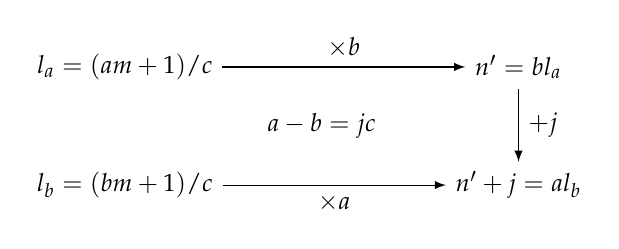
\begin{tikzpicture}[>=latex, every node/.style={font=\small}]
\node (la) at (0,0) {$l_a=(am+1)/c$};
\node (lb) at (0,-1.5) {$l_b=(bm+1)/c$};
\node (np) at (5,0) {$n'=bl_a$};
\node (nj) at (5,-1.5) {$n'+j=al_b$};
\draw[->] (la) -- node[above] {$\times b$} (np);
\draw[->] (lb) -- node[below] {$\times a$} (nj);
\draw[->] (np) -- node[right] {$+j$} (nj);
\node at (2.5,-0.75) {$a-b=jc$};
\end{tikzpicture}
\caption{The exact reindexing of two divisor representations. The
coefficient identity makes the new endpoints differ by $j$, while
fixed-multiplier invariance preserves their centered labels.}
\label{fig:graph-reindexing}
\end{figure}

For fixed $B$, the coefficient supports are finite, so
\eqref{eq:labels-multiplier} applies simultaneously to the multipliers
$c,b,a$ once $x$ is sufficiently large. Removing $c$ and then inserting
$b,a$ gives
\[
 \overline{F_x(am+1)}F_x(bm+1)
 =\overline{F_x(l_a)}F_x(l_b)
 =\overline{F_x(n')}F_x(n'+j).
\]
Define
\[
 \Psi_s(u_1,u_2)=
 \psi(u_1)\psi(u_2)\phi(s/u_1)\phi(s/u_2).
\]
If $s=n'/(Tx)$, $u_1=a/(Tc)$ and $u_2=b/(Tc)$, then
\[
 s/u_1=bm/x+b/(ax),\qquad s/u_2=am/x+1/x.
\]
The two original $\phi$-arguments are therefore interchanged, with
errors $O_B(1/x)$. Since they occur as a product, their replacement by
$\Psi_s$ has vanishing error for fixed $B$. There is a fixed compact
interval $\mathcal S\subset(0,\infty)$ outside which $\Psi_s$ vanishes
on the coefficient supports. It depends only on $\phi,\psi$.

Consequently, the off-diagonal part of $I_{2,x}/(BT)$ is, up to $o_x(1)$,
\begin{equation}\label{eq:16}
 \frac1{Tx}\sum_{n'}\sum_{0<|j|\le T}
 \overline{F_x(n')}F_x(n'+j)
       \mathcal K_j(n',n'/(Tx)),
\end{equation}
where, for $u\in\whZ$,
\begin{equation}\label{eq:17}
\begin{split}
 \mathcal K_j(u,s)=\frac1B
 \sum_{\substack{a-b=jc,\ (a,b)=(a,c)=(b,c)=1\\
                  b\mid u,\ a\mid u+j}}
 &A(a)A(b)A(c)K(u/b)K((u+j)/a)\\[-2pt]
 &\quad\cdot K\!\left(\frac{c(u/b)-1}{a}\right)
 \rho_0(\log c/B)\Psi_s(a/(Tc),b/(Tc)).
\end{split}
\end{equation}
All coefficient variables are positive integers. Divisibility in
$\whZ$ means membership in the image of multiplication by the
divisor; that multiplication is injective. The preceding congruence
calculation also proves that every quotient in \eqref{eq:17} is
defined on its summation domain. This kernel is nonnegative, depends
on finitely many prime-power residues, and satisfies
\[
 \mathcal K_j(u,s)=\mathcal K_{-j}(u+j,s).
\]
For this last identity, exchange $a,b$: the last quotient is unchanged
because $c(u+j)-a=cu-b$.

\begin{lemma}[Mean edge mass]\label{lem:graph-edge-mass}
Uniformly for $0<|j|\le T$ and $s\in\mathcal S$,
\begin{equation}\label{eq:18}
 \E_{u\in\whZ}\mathcal K_j(u,s)\ll\frac{\Sigma(j)}T.
\end{equation}
The implied constant can be independent of the regularity parameter
$C_*$.
\end{lemma}

\begin{proof}
Replace all truncated weights by their untruncated majorants.
For fixed pairwise coprime $a,b,c$, the two endpoint congruences have
Haar probability $1/(ab)$. At a prime $p\in\mathcal P$ not dividing
$abc$, the three residue weights have distinct zero classes
$0,-j,b/c$ for $u$. Here $p>|j|$, and $b/c\not\equiv-j\pmod p$
follows from $a=b+jc$. Their local mean is $1-3/(2p)$.
At primes dividing $abc$ discard the local reducing factors; this
changes the Euler-product bound by at most
$\exp(O(\sum_{p\mid abc}1/p))=O(1)$, since that sum is $O(B/P_0)$.
Independence over primes and Mertens' formula give
\[
 R^{3/2}\prod_{p\in\mathcal P}(1-3/(2p))\ll1.
\]
On a dyadic box $c\asymp X$, the denominator is
$ab\asymp T^2X^2$. The three-form estimate \eqref{eq:7} bounds its
contribution before the factor $1/B$ by $O(\Sigma(j)/T)$.
There are $O(B)$ boxes. This proves the assertion using only
untruncated upper bounds.
\end{proof}

\subsection{Blocks and the norm used for comparison}

Fix $0<\eta<1$ and $C_6>1$, and set $M=\lceil C_6T\rceil$.
Removing the lags $|j|<\eta T$ in \eqref{eq:16} costs
$O(\eta)+o_x(1)$ in absolute upper limit, by
Lemma~\ref{lem:graph-edge-mass} and the bounded ordinary averages of
$\Sigma$. Average the origins over $i=1,\ldots,M$, writing
$n'=n+i$. For fixed $B$, replacing $(n+i)/(Tx)$ by $n/(Tx)$
has vanishing error. At lag $j$, the fraction of $i$ for which
$k=i+j\notin[1,M]$ is at most $|j|/M$. The total cost of these
endpoints is $O(T/M)=O(1/C_6)$. The remaining expression is
\begin{equation}\label{eq:19}
 \mathcal Q^{\mathrm{arith}}_{B,x}:=\frac1{Tx}\sum_n\frac1M
 \sum_{\substack{1\le i,k\le M\\\eta T\le|k-i|\le T}}
 \overline{F_x(n+i)}F_x(n+k)
 \mathcal K_{k-i}(n+i,n/(Tx)).
\end{equation}
Thus \eqref{eq:15} and the diagonal estimate give a positive lower
bound for the iterated lower limit of \eqref{eq:19}, once $\eta$ is
small enough and $C_6$ is large enough. These choices are made after
$C_*$ and before letting $B$ grow.

Call a pair $(i,k)$ \emph{allowed} if
$1\le i,k\le M$ and $\eta T\le|k-i|\le T$. All matrices below are
zero on other pairs. For a real matrix $H$, define
\begin{equation}\label{eq:graph-cutnorm}
 \|H\|_\square=
 \frac1M\max_{\epsilon,\delta\in\{-1,1\}^M}
 \left|\sum_{i,k}H_{ik}\epsilon_i\delta_k\right|.
\end{equation}
The same maximum results from allowing real test coordinates in
$[-1,1]$. Splitting real and imaginary parts shows that for complex
$z_i$ with $|z_i|\le2$,
\begin{equation}\label{eq:graph-cut-labels}
 \left|\frac1M\sum_{i,k}H_{ik}\overline{z_i}z_k\right|
 \le16\|H\|_\square.
\end{equation}
For fixed $B$, a matrix whose entries are finite-residue functions
continuous in $s$ has the same property after taking this finite
maximum. Its ordinary scale averages converge to its Haar-product
integral. Therefore bounds on the Haar expectation of the norm,
uniformly for $s\in\mathcal S$, control errors in
\eqref{eq:19}. This comparison is deterministic in the labels; it
requires no independence between the labels and the residue data.

\subsection{Endpoint types and candidate representations}

The block energy is now expressed in the norm that will control its
approximation. We next separate the prime-divisibility data at the endpoints
from the additional residue data belonging to each edge representation.

Put $S_i(u)=\{p\in\mathcal P:p\mid u+i\}$. We compare them with
independent sets $S_i$, each formed by independently including every
$p\in\mathcal P$ with probability $1/p$. At a fixed $p>P_0>M$,
the actual law has disjoint hits of probability $1/p$ at each site.
Its total variation distance from independent hits is
$O(M^2/p^2)$. Consequently the joint site laws can be coupled with
failure probability $O(M^2/P_0)$. Also
\begin{equation}\label{eq:graph-site-squares}
 \Prob\{p^2\mid u+i\text{ for some }p\in\mathcal P,\ i\le M\}
 \ll M/P_0.
\end{equation}

For an allowed pair $i,k=i+j$ with $j>0$, a \emph{candidate}
consists of a subset product $b$ of $S_i$, a subset product $a$ of
$S_k$, and the positive integer $c=(a-b)/j$. Require pairwise
coprimality, rough squarefreeness, all three coefficient regularity
conditions, and regularity of the two remaining sets
$S_i\setminus b$ and $S_k\setminus a$. Here $S\setminus b$
means removal of the primes dividing $b$. It is harmless to use
the closed support windows
\[
 B\le\log c\le2B,\qquad Tc\le a,b\le2Tc;
\]
the smooth factors still impose the original supports. A reversed
ordered pair refers to the same candidate.

A contributing endpoint has at most $(1+2\tau)\ell$ primes.
There are at most $2^{2(1+2\tau)\ell}$ subset choices at a pair,
so the number of candidates in the entire block is $O(B^4)$.
This rough bound also applies to representations that contribute to
\eqref{eq:17} in the presence of site squares: the union of the
coefficient and quotient prime sets covers the site's distinct
primes, and their total-count restrictions give the same bound.
Together with \eqref{eq:8}, this gives, for example, a deterministic
$O(B^{10})$ bound for all total matrix masses used below. This bound
allows small-probability errors to be discarded before sharper mean
estimates are available.

Set $k_B=\E_S K(S)$ under the independent $1/p$ law. The
untruncated Euler product gives $k_B\ll1$. Define the latent kernel
\begin{equation}\label{eq:20}
\begin{split}
 \mathcal L_{ik}(S_i,S_k;s)=\frac{k_B}{B}
 \sum_{\text{candidates}}&A(a)A(b)A(c)
 K(S_i\setminus b)K(S_k\setminus a)\\[-2pt]
 &\quad\cdot\rho_0(\log c/B)\Psi_s(a/(Tc),b/(Tc)),
\end{split}
\end{equation}
and extend it by symmetry and by zero on nonpairs.
For actual endpoint sets without site squares, the terms allowed by the
smooth factors have the same coefficient representations in
\eqref{eq:17} and \eqref{eq:20}, and the two endpoint quotient prime sets
are the complementary sets displayed in \eqref{eq:20}. The latter kernel
keeps these terms and replaces the remaining factor $K(m)$ by its
independent mean $k_B$.

\begin{lemma}[Uniform conditional means]\label{lem:graph-row-mean}
For every possible endpoint type $S_i$, not merely almost every
typical type, and every allowed lag $j=k-i$,
\begin{equation}\label{eq:23}
 \E_{S_k}\mathcal L_{ik}(S_i,S_k;s)
 \ll\frac{\Sigma(j)}T.
\end{equation}
In particular, every conditional expected degree is $O(1)$, and
$\E\sum_{i,k}\mathcal L_{ik}=O(M)$.
\end{lemma}

\begin{proof}
For an admissible fair split $b$ at the first endpoint,
$A(b)K(S_i\setminus b)=B2^{-|S_i|}$. At the other endpoint,
the analogous identity and then averaging over its site set give
the split-product law $\nu_{1/2}$. By \eqref{eq:4}, its mass at
$a$ is at most $CA_0(a)/(Ba)$. Dropping all remaining restrictions
for an upper bound yields
\begin{align*}
 \E_{S_k}\mathcal L_{ik}(S_i,S_k;s)
 &\ll \E_{b\mid S_i,\,\mathrm{split}}
 \ind_{\{b\text{ in the possible range}\}}
 \sum_{\substack{c\asymp b/T,\ a=b+jc\asymp b\\B\le\log c\le2B}}
       \frac{A_0(c)A_0(a)}a\\
 &\ll\frac{\Sigma(j)}T
 \E_{b\mid S_i,\,\mathrm{split}}
       \ind_{\{b\text{ in the possible range}\}}
 \le C\frac{\Sigma(j)}T,
\end{align*}
using \eqref{eq:6}. This is a restricted expectation of mass at
most one, with no division by its probability. If the fixed type
has no admissible split, its kernel is zero. The same estimate
with signed lag reversed handles either endpoint. Summing the
bounded averages of $\Sigma$ proves the degree assertions.
\end{proof}

\subsection{Separating the auxiliary roots}

The following comparison justifies this averaging in expected cut norm,
uniformly against a proposed endpoint
kernel. It is stronger than an estimate against any one predetermined
pair of tests.

\begin{proposition}[Independent-root comparison]
\label{prop:graph-root-comparison}
Let $\mathcal M_{ik}(S_i,S_k;s)$ be a symmetric real kernel,
zero on nonpairs, with total absolute mass $O(B^{10})$
uniformly in its arguments. Then
\begin{equation}\label{eq:21}
\begin{split}
 &\E_u\left\|
  \bigl(\mathcal K_{k-i}(u+i,s)
  -\mathcal M_{ik}(S_i(u),S_k(u);s)\bigr)_{i,k}
  \right\|_\square\\
 &\hspace{15pt}\le o(1)+
 \E_{(S_i)\,\mathrm{indep}}
 \left\|\bigl(\mathcal L_{ik}(S_i,S_k;s)
                   -\mathcal M_{ik}(S_i,S_k;s)\bigr)_{i,k}\right\|_\square.
\end{split}
\end{equation}
The error is uniform for $s\in\mathcal S$.
\end{proposition}

\begin{proof}
In the absence of site squares, quotient prime sets at the
endpoints equal the complementary sets used in \eqref{eq:20}.
For a candidate at $i,k=i+j$, the remaining argument in
\eqref{eq:17} is
\begin{equation}\label{eq:22}
 m=\frac{c(u+i)-b}{ab}
   =\frac{c}{ab}(u-r),\qquad r=b/c-i=a/c-k.
\end{equation}
We show that, at a negligible total error, the set of primes
dividing this argument can be replaced for each unordered
candidate by an independent $1/p$ set, independent of the site
sets and of the other candidates' extra sets. The following
argument first bounds two obstructions determined by the endpoint sets:
coincident rational roots and a root forced to hit a third occupied site.
It then fixes a surviving actual site configuration and couples the
remaining prime tests, without conditioning on absence of site squares.
The site-square event is paid for in the matrix weights, and the final
step controls the independent extra-weight fluctuations in cut norm.

\paragraph{Coincident rational roots.}
Since $b/c$ is reduced, equal $r$ for two candidates forces the
same denominator $c$. Given $r,c$, the coefficient at any
position $s'$ is fixed, namely $b+(s'-i)c$. On the same pair
this determines the candidate uniquely. Any other unordered
pair with this root uses at least a third position with a
prescribed positive coefficient at least $Tc$. Conditional on
the first two independent site sets, that coefficient is
available at the third site with probability at most $1/(Tc)$:
it has probability zero unless it is a squarefree product of
$\mathcal P$ primes, and otherwise the probability is its
reciprocal. The polynomial candidate and position bounds,
and $c\ge e^B$, make the union of these events negligible.
The site coupling transfers the conclusion to the actual model.

\paragraph{Forced hits at a third endpoint.}
Also discard the event that, for some candidate and
$s'\ne i,k$, an occupied prime $p$ at site $s'$ satisfies
$p\nmid abc$ and $r\equiv-s'\pmod p$.
In the independent-site model, condition on the candidate's
two endpoint sets. Such a prime divides
$b+(s'-i)c$, a nonzero integer of logarithmic size $O(B)$.
It is nonzero because $c>1$ and $(b,c)=1$.
For any nonzero integer of logarithmic size $O(B)$, the sum
of reciprocals of its prime divisors above $P_0$ is
$O(B/P_0)$. Thus the conditional union probability is
$O(B/P_0)$ per candidate and third position. A polynomial
union bound and the site coupling again suffice.

\paragraph{Coefficient primes and occupied primes.}
The two structural exclusions above depend only on the endpoint sets,
and their actual-law probabilities have been bounded through the site
coupling. Fix an actual site configuration avoiding them; its hits at
each prime are disjoint. We still do not condition on absence of site
squares. At an unoccupied prime, $u\bmod p$ is uniform
outside the $M$ forbidden classes $-1,\ldots,-M$.
At an occupied prime, its residue is fixed and the higher
$p$-adic digits remain uniform. These conditional laws are
independent over primes.

If $p\mid ab$, then the coefficients are squarefree and
pairwise coprime, and the test $p\mid m$ in \eqref{eq:22}
has conditional probability $1/p$, determined by the next
digit. If $p\mid c$, it is impossible. Set these exceptional
tests to zero temporarily, in both the actual model and the
independent comparison model. The total error per candidate
is $O(B/P_0)$. This use of uniform higher digits is made
before removing site-square events from the weights; we
do not condition those digits on absence of squares.

At $p\nmid abc$, the root test is $u\equiv r\pmod p$.
If the prime is occupied at an endpoint, such coincidence
would force $p\mid b$ or $p\mid a$. At any other occupied
site it is excluded by the preceding discarded event.
The actual root test is therefore zero at the remaining
occupied primes. The cost of setting the independent test
to zero there is bounded in expectation by the deterministic
candidate bound times
\[
 \E\sum_{p\text{ occupied}}\frac1p
 \le M\sum_{p>P_0}\frac1{p^2}.
\]
This domination does not require candidates to be independent
of occupied primes.

\paragraph{Unoccupied primes.}
The roots are now distinct rational numbers. A collision
between two of their residues modulo $p$, after excluding
coefficient primes, requires $p$ to divide their nonzero
cross-multiplied difference. That integer has logarithmic
size $O(B)$. A collision with a forbidden site class has
the same bound, or concerns a coefficient prime already
handled. For each candidate pair or candidate--site pair,
these defective primes have reciprocal sum $O(B/P_0)$.
At all such primes, discard all involved tests. Conditional
on the sites, each defined test has probability at most
$1/(p-M)\le2/p$, so another polynomial loss is harmless.

At a remaining unoccupied prime the root classes are
distinct and avoid all forbidden classes. Their joint law
is a disjoint-choice law with individual hit probabilities
$1/(p-M)$. If there are $N_{\rm cand}=O(B^4)$ tests, its
total variation distance from independent Bernoulli$(1/p)$
tests is
\[
 O\!\left(\frac{(M+N_{\rm cand})^2}{p^2}\right).
\]
For example, compare first to independent tests of probability
$1/(p-M)$, at cost $O(N_{\rm cand}^2/p^2)$ from multiple
hits, and then change each probability to $1/p$, at cost
$O(N_{\rm cand}M/p^2)$. Summing over primes constructs the
claimed conditional coupling. The preceding union bounds give total
failure probability $O(B^{C}/P_0)+O(B^{C}e^{-B})$ for a fixed crude
exponent $C$. On these failures, use the deterministic polynomial
matrix-mass bounds. After including that loss and enlarging the crude
exponent, their contribution to the expected cut norm is at most
$O(B^{50}/P_0)+O(B^{50}e^{-B})=o(1)$.
Equation~\eqref{eq:graph-site-squares}
is handled in the resulting weights, as just explained.

\paragraph{Fluctuations of the extra weights.}
The preceding coupling has separated the extra roots from the endpoint
types. It remains to show that their independent fluctuations are small
even after maximizing the testing signs.
The comparison model has independent endpoint types and
an additional independent set $S_{\rm root}$ for each
unordered candidate. In its weight, replace $k_B$ in
\eqref{eq:20} by $K(S_{\rm root})$. Conditional on the
endpoints, the candidate weights are independent, and
their means give precisely $\mathcal L$. By
\eqref{eq:8}, each full candidate weight, including its
six truncated factors and the factor $1/B$, is at most
\[
 C B^{-1+6(h_0+\tau\log2)+o(1)}\le B^{-0.07}
\]
for large $B$, with harmless enlargement of constants.
For fixed sign vectors in \eqref{eq:graph-cutnorm}, an
unordered candidate has sign coefficient of absolute
value at most two. Positivity bounds the conditional
variance sum by a constant times $B^{-0.07}$ times
$\sum_{i,k}\mathcal L_{ik}$.

Bernstein's inequality, union over at most $2^{2M}$
sign choices, and integration of the tail show that the
conditional expected cut norm of the centered fluctuation
is at most
\begin{equation}\label{eq:graph-root-fluctuation}
 C\left(
 \sqrt{B^{-0.07}\frac1M\sum_{i,k}\mathcal L_{ik}}
 +B^{-0.07}\right).
\end{equation}
Indeed, before division by $M$, a threshold
\[
 C\left(
 \sqrt{B^{-0.07}\Bigl(\sum_{i,k}\mathcal L_{ik}\Bigr)(M+y)}
 +B^{-0.07}(M+y)\right)
\]
has tail $O(e^{-y})$ for $y\ge0$, with $C$ absorbing
the sign enumeration. Lemma~\ref{lem:graph-row-mean}
and Jensen's inequality make the expectation of
\eqref{eq:graph-root-fluctuation} tend to zero.
The triangle inequality now proves \eqref{eq:21}; the
deterministic polynomial mass bounds control the coupling
failures for both kernels. All estimates used only uniform
bounds for the smooth factors on $\mathcal S$.
\end{proof}

\section{A second moment for the latent rows}
\label{sec:moments}

The independent-root comparison leaves the latent kernel
$\mathcal L$ of \eqref{eq:20}.  Its conditional first moments are bounded
uniformly over every site type by \eqref{eq:23}.  For the sampling argument
we also need an integrated second-moment estimate.  A small bound on each
individual representation does not suffice, because an edge may have
several representations. Expanding the square and weighting one
representation will identify the measure under which that multiplicity
must be controlled.

The grid size $L$ and tolerance $\tau$ will be chosen once below,
consistently with Section~\ref{sec:arithmetic}. In every limit
$B\to\infty$ in this section, those choices, $\eta>0$, the block constant
$C_6$, $C_*$, and the smooth weights are held fixed.
All estimates are uniform in the positions and in the smooth parameter
$s$ on the fixed compact range used in Section~\ref{sec:graph}.
Constants may depend on the fixed parameters but not on the particular
first representation.

\begin{proposition}[Integrated row moments]
\label{prop:moments:rows}
For a sufficiently fine fixed regularity grid and then a sufficiently
small fixed tolerance, the independent-site latent kernel satisfies
\begin{equation}
 \sum_{k\ne i}\E\,\mathcal L_{ik}^{2}\ll B^{-.21}
 \qquad (1\le i\le M).
 \label{eq:24}
\end{equation}
Moreover, its normalized total mass has bounded second moment:
\[
 \E\left(\frac1M\sum_{i,k}\mathcal L_{ik}\right)^2\ll1.
\]
For every set $I\subseteq\{1,\ldots,M\}$, the same estimates hold after
replacing $\mathcal L_{ik}$ by
$\ind_{\{i,k\in I\}}\mathcal L_{ik}$; the normalization remains $M$.
\end{proposition}

Write $h_\tau=h_0+\tau\log2$.  There are five truncated weights in
an individual summand of \eqref{eq:20}.  Since $k_B\ll1$ and the smooth
factors are bounded, \eqref{eq:8} gives the uniform bound
\begin{equation}
\begin{gathered}
 \text{one contribution to }\mathcal L_{ik}
 \ \le B^{-\kappa_1+5\tau\log2+o(1)},
 \\
 \kappa_1=1-5h_0=0.232867951\ldots> .2328.
 \label{eq:25}
\end{gathered}
\end{equation}
\subsection{The measure obtained from a first representation}

Fix an allowed pair $i,k=i+j$. Let
$\mathcal C_j$ be the finite set of positive triples $(a,b,c)$ satisfying
\[
 a-b=jc,\qquad
 B\le\log c\le2B,\qquad Tc\le a,b\le2Tc,
\]
whose entries are pairwise coprime, rough, squarefree, and regular.
These are precisely the coefficient conditions for a candidate; the
two remainder regularity conditions still depend on the site types.
We initially take $j>0$; the negative case follows by exchanging the
endpoints. Fix $(a,b,c)\in\mathcal C_j$. For an integer $v$ whose prime
factors belong to $\mathcal P$, write $\mathcal P(v)$ for its set of prime
factors.

In the independent-site model, the event
$\mathcal P(b)\subset S_i$, $\mathcal P(a)\subset S_k$ has probability
$1/(ab)$.  Conditional on that event, put
\[
 \mathcal T_b=S_i\setminus\mathcal P(b),
 \qquad
 \mathcal T_a=S_k\setminus\mathcal P(a).
\]
These sets are independent, and at each prime not excluded by the
corresponding coefficient the inclusion probability is $1/p$.
Weighting one such inclusion by its factor $1/2$ in $K_0$ changes this
probability to
\[
 \frac{(1/p)/2}{1-1/(2p)}=\frac1{2p-1}.
\]
Thus weighting by $K_0(\mathcal T_b)K_0(\mathcal T_a)$ gives a product
probability measure, denoted by $\Prob^{\mathrm{tilt}}_{a,b}$, under which
the two remainder sets are independent and their available prime
indicators have probabilities $1/(2p-1)$.

For a coefficient $v$ the normalizing factor is
\[
 \Xi(v)=R^{1/2}
       \prod_{p\in\mathcal P\setminus\mathcal P(v)}
                    \left(1-\frac1{2p}\right).
\]
The full product with no exclusions is bounded by Mertens' estimate.
Furthermore $\log v=O(B)$ and every prime of $v$ exceeds $P_0$, so
\[
 \sum_{p\mid v}\frac1p\ll\frac{B}{P_0}.
\]
Removing these factors changes the product by $1+o(1)$.  Consequently
$\Xi(v)\ll1$ uniformly for the coefficients under consideration.
For every nonnegative function $H$ of the two remainder sets we therefore
have the exact change-of-measure identity
\[
 \begin{split}
 &\E\big[
   \ind_{\mathcal P(b)\subset S_i,\,\mathcal P(a)\subset S_k}
   K_0(\mathcal T_b)K_0(\mathcal T_a)H(\mathcal T_b,\mathcal T_a)
       \big]\\
 &\hspace{25mm}
   =\frac{\Xi(b)\Xi(a)}{ab}
       \E^{\mathrm{tilt}}_{a,b}H(\mathcal T_b,\mathcal T_a).
 \end{split}
\]
The indicators that the two first remainders are regular will stay
inside $H$.  In particular, we never divide by their probability.

Given these remainder sets, reconstruct
$S_i=\mathcal P(b)\cup\mathcal T_b$ and
$S_k=\mathcal P(a)\cup\mathcal T_a$, and let
$N_{a,b,c}(\mathcal T_b,\mathcal T_a)$ be the number of valid candidates
at this pair for the reconstructed types, including the first triple
whenever it is valid.

We can now see exactly how this measure enters the square.
Expand the square of the sum of nonnegative candidate contributions,
designate one candidate as the first representation, and bound every
alternative contribution by \eqref{eq:25}. The first contribution retains
the two factors $K_0(\mathcal T_b)K_0(\mathcal T_a)$ and their regularity
indicators. The change-of-measure identity gives
\begin{equation}
\begin{split}
 \E\,\mathcal L_{ik}^{2}
 &\ll B^{-\kappa_1+5\tau\log2+o(1)}
 \frac1B\sum_{(a,b,c)\in\mathcal C_j}
       \frac{A(a)A(b)A(c)}{ab}\,\Xi(a)\Xi(b)\\
 &\qquad\cdot
 \E^{\mathrm{tilt}}_{a,b}
 \big[
   \ind_{\mathcal T_b\ \mathrm{regular}}
   \ind_{\mathcal T_a\ \mathrm{regular}}
   N_{a,b,c}(\mathcal T_b,\mathcal T_a)
 \big].
\end{split}
\label{eq:moments-first-representation}
\end{equation}
The implied constant absorbs $k_B$ and the bounded smooth factors.
Thus the remaining multiplicity question is the following uniform
estimate; the coefficient sum will then be bounded by \eqref{eq:7}.

\begin{lemma}[Weighted representation multiplicity]
\label{lem:moments:multiplicity}
The grid and tolerance can be chosen so that, uniformly for
$(a,b,c)\in\mathcal C_j$ and $\eta T\le |j|\le T$,
\[
 \E^{\mathrm{tilt}}_{a,b}
   \big[
    \ind_{\mathcal T_b\ \mathrm{regular}}
    \ind_{\mathcal T_a\ \mathrm{regular}}
    N_{a,b,c}(\mathcal T_b,\mathcal T_a)
   \big]
 \ll B^{.009}.
\]
\end{lemma}

\begin{proof}
Every alternative candidate has a unique decomposition
\[
 b'=d_1y,\quad d_1\mid b,\quad\mathcal P(y)\subset\mathcal T_b,
 \qquad
 a'=e_1z,\quad e_1\mid a,\quad\mathcal P(z)\subset\mathcal T_a,
 \qquad a'-b'=jc'.
\]
Here all the products are squarefree, and $y$ is coprime to $b$ while
$z$ is coprime to $a$.  The coefficient $c'$ is determined once the
four products are chosen.  We may discard any of the alternative
candidate conditions for upper bounds; however, we retain the
coefficient regularity conditions that are used below.  Since
$a',b'\le2T\exp(2B)$, we have $\log y,\log z\le3B$ for all sufficiently
large $B$.

Set $\Delta=1/L$, $g_0=3\Delta$, and
$U=\max(\log y,\log z)$. We count the alternatives with
$U\le B^{g_0}$ directly from prefix regularity. When $U>B^{g_0}$,
fixing the omissions and the new product at one endpoint places the
other new product in one residue class modulo $|j|$, through
$e_1z-d_1y=jc'$. The resulting progression density is the gain that
will pay for the remaining subset choices.

For a grid point $g<1$, define
\[
 \mathcal Q_g=\{p\in\mathcal P:\log p\le B^g\},
 \qquad \mathcal Q_1=\mathcal P,
\]
and write $\omega_g(v)=|\mathcal P(v)\cap\mathcal Q_g|$, with the
same notation for a prime set.  Regularity gives
\[
 (g/2-\tau)\ell\le\omega_g(v)\le(g/2+\tau)\ell
\]
for each of the first and alternative coefficients, and for each
regular first remainder.  Mertens' estimate, on this fixed grid, gives
\[
 \sum_{p\in\mathcal Q_g}\frac1p=g\ell+o(\ell).
\]
The $o(\ell)$ is uniform over the finitely many grid points.

\paragraph{Omissions above an addition prefix.}
Suppose that all primes of $z$ and $y$ lie in $\mathcal Q_g$.
Let $D_a=\mathcal P(a)\setminus\mathcal P(e_1)$ be the primes omitted
from $a$.  Regularity of the total counts of $a,a'$ gives
\[
 \bigl||D_a|-\omega(z)\bigr|\le2\tau\ell.
\]
Regularity at $g$ gives the analogous inequality
\[
 \bigl||D_a\cap\mathcal Q_g|-\omega(z)\bigr|\le2\tau\ell.
\]
Subtracting shows that at most $4\tau\ell$ primes above the prefix
can be omitted.  The same conclusion holds for the omissions from $b$.
When $g=1$ there are no primes above the prefix.

Write
\[
 H(u)=-u\log u-(1-u)\log(1-u),\qquad 0\le u\le1,
\]
with the endpoint values defined by continuity.
For completeness, if $m\le8\tau\ell$, the number of such subsets is
at most $2^m\le2^{8\tau\ell}$.  For
$8\tau\ell<m\le(1/2+\tau)\ell$, the binomial bound
\[
 \sum_{q\le4\tau\ell}\binom mq
 \le (m+1)\exp\bigl(mH(4\tau\ell/m)\bigr)
 \le (m+1)\exp\left((1/2+\tau)\ell
                 H\left(\frac{4\tau}{1/2+\tau}\right)\right)
\]
applies: $H$ is increasing up to $1/2$, and $mH(k/m)$ is increasing
in $m$ for fixed $0<k<m$.  Thus the choices at both coefficients
together cost $B^{\varepsilon_{\mathrm{high}}(\tau)+o(1)}$, where
$\varepsilon_{\mathrm{high}}(\tau)\to0$ as $\tau\to0$.
The estimate is uniform also when the relevant set is empty.

\paragraph{Small additions.}
If
\[
 U\le B^{g_0},
\]
all additions lie in $\mathcal Q_{g_0}$.  On the two first-remainder
regularity events, the four relevant prefix sets---the prime sets of
$a,b$ and the two first remainders---have at most
$(2g_0+4\tau)\ell$ primes altogether.  Allowing arbitrary subset choices
there, and then the higher omissions just bounded, gives the
pointwise estimate
\[
 N_{\mathrm{small}}
 \le 2^{(2g_0+4\tau)\ell}
       B^{\varepsilon_{\mathrm{high}}(\tau)+o(1)}
 =B^{(2g_0+4\tau)\log2+
                  \varepsilon_{\mathrm{high}}(\tau)+o(1)}.
\]
This also bounds its expectation with the first-remainder regularity
indicators.  By taking $L$ large and then $\tau$ small, its exponent
apart from $o(1)$ can be made strictly smaller than $.008$.

\paragraph{Large-addition classes and combinatorial choices.}
For $U>B^{g_0}$ use the classes
\[
 B^{g-\Delta}<U\le B^g
       \quad(g_0<g<1),
 \qquad
 B^{1-\Delta}<U\le3B\quad(g=1),
\]
where $g$ ranges over grid points.  All addition primes again belong to
$\mathcal Q_g$.  It suffices to treat the portion of a class in which
$\log z>B^{g-\Delta}$.  The portion with $\log y>B^{g-\Delta}$ is
estimated by the same argument with the endpoints exchanged; the
numeric sieve below permits either sign for its second slope.  If both
inequalities hold, counting the alternative twice only increases the
upper bound.

Define the exact normalized counts and their clipped values by
\[
 r_z^* =\frac{\omega(z)}{g\ell},\qquad
 r_y^* =\frac{\omega(y)}{g\ell},\qquad
 r_z=\min(r_z^*,1/2),\qquad r_y=\min(r_y^*,1/2).
\]
On the first-remainder regularity events,
$0\le r_z^*,r_y^*\le1/2+\tau/g$.  There are $O(\ell^2)$ possible pairs of
integer counts.  We estimate one such pair at a time.

The number of omitted primes in the $a$ prefix is
$r_z^*g\ell+O(\tau\ell)$, among
$g\ell/2+O(\tau\ell)$ available primes.  Applying
$\binom mq\le\exp(mH(q/m))$, and summing over the $O(\ell)$ permissible
values of $q$, gives, with the higher-omission factor included,
\begin{equation}
 \#\{e_1\}\le
 B^{\frac12 gH(2r_z)+\varepsilon_L(\tau)+o(1)}.
 \label{eq:26}
\end{equation}
The function $\varepsilon_L(\tau)$ can be chosen to tend to zero for
fixed $L$.  To justify this uniformly in the counts, divide $m,q$ by
$\ell$ and use uniform continuity of $H$ on $[0,1]$; the perturbations
are $O(\tau/g)$, and $g\ge g_0>0$ is fixed.  The clipping from $r_z^*$ to
$r_z$ changes these arguments by the same amount.  Also
$\ell/\log B\to1$, and all polynomial factors in $\ell$ contribute
$B^{o(1)}$.  We use $\varepsilon_L(\tau)$ below for a possibly enlarged
function with this same limiting property.

The choices of $d_1$ have the corresponding bound with $r_y$.
Conditional on a regular first remainder $\mathcal T_b$, the number
of its subsets $y$ of the prescribed cardinality is at most
\[
 B^{\frac12 gH(2r_y)+\varepsilon_L(\tau)+o(1)}.
\]
This bound is uniform in that remainder set.  We may condition on it
and sum over these $y$ while the remainder at the other endpoint still
has its independent tilted law.

\paragraph{Availability of a fixed numeric addition.}
The entropy bounds count the possible omitted prime sets. To control
large additions, we also need the probability that each numerically
specified product is present in the other remainder set. The next bound
keeps the first remainder's regularity requirement in this probability.
For a fixed squarefree $z$ in this class, with
$\mathcal P(z)\subset\mathcal Q_g\setminus\mathcal P(a)$, its inclusion
probability in $\mathcal T_a$ is
\[
 \prod_{p\mid z}\frac1{2p-1}
 =\frac{2^{-\omega(z)}}{z}
       \prod_{p\mid z}\left(1-\frac1{2p}\right)^{-1}
 \ll \frac{2^{-\omega(z)}}{z}.
\]
The last bound is uniform because $\log z\le3B$ and all its primes
exceed $P_0$.  Conditional on those inclusions, the remaining available
indicators in $\mathcal Q_g$ are independent with parameter sum
\[
 \Lambda=\sum_{p\in\mathcal Q_g\setminus
                       (\mathcal P(a)\cup\mathcal P(z))}
                       \frac1{2p-1}
         =\tfrac12g\ell+o(\ell).
\]
The excluded primes have reciprocal sum $O(B/P_0)$, so this estimate
is uniform in the fixed coefficient and numeric addition.  First
prefix regularity requires the number of these other inclusions to be
at most $(1/2-r_z^*)g\ell+\tau\ell$.

If $X$ is a sum of independent Bernoulli variables with parameter sum
$\Lambda$, then for $t\ge0$,
\[
 \Prob(X\le k)
 \le\exp\bigl(tk+(e^{-t}-1)\Lambda\bigr).
\]
For $0\le k\le\Lambda$, minimizing gives exponent
$-\Lambda+k-k\log(k/\Lambda)$, with its continuous value at $k=0$.
For $k\ge\Lambda$ use the bound $1$, and for $k<0$ the event is empty.
Uniform continuity of the resulting rate, including the endpoints,
and the fixed-grid relation $g\ge g_0$ therefore imply
\begin{equation}
 \begin{split}
 &\Prob^{\mathrm{tilt}}_{a,b}
   \bigl(\mathcal P(z)\subset\mathcal T_a,
              \ \mathcal T_a\text{ regular at }g\bigr)\\
 &\hspace{12mm}\ll
   \frac{(1/2)^{\omega(z)}}{z}
       B^{-gI_{1/2}(1/2-r_z)+\varepsilon_L(\tau)+o(1)},
 \qquad
 I_{1/2}(u)=\tfrac12-u+u\log\frac{u}{1/2}.
 \end{split}
 \label{eq:27}
\end{equation}
Here $u\log u=0$ at $u=0$.  Retaining only prefix regularity on the
left gives an upper bound for retaining all of first-remainder
regularity, which is what the multiplicity expectation requires.

\paragraph{A harmonic sieve for the numeric addition.}
We now sum the availability bound over numeric additions satisfying
the alternative coefficient relation. The factor $1/z$ in that bound
is the reason for the harmonic normalization below.
Fix $e_1,d_1,y$ from the preceding choices. The alternative size
conditions imply
\[
 z\asymp Z':=d_1y/e_1
\]
with absolute comparison constants; we may enlarge the interval to
$[Z'/2,2Z']$.

For these fixed data and the fixed cardinality class, let
$\mathcal Z$ consist of the positive integers $z$ with the following
properties:
\[
\begin{gathered}
 z\text{ is a squarefree product of primes in }
       \mathcal Q_g\setminus\mathcal P(a),\qquad
 \omega(z)=r_z^*g\ell,\\
 Z'/2\le z\le2Z',\qquad
 \log z\in
 \begin{cases}
 (B^{g-\Delta},B^g],&g<1,\\
 (B^{1-\Delta},3B],&g=1,
 \end{cases}\\
 e_1z\equiv d_1y\pmod{|j|},\qquad
 c'(z):=\frac{e_1z-d_1y}{j}>0,\qquad
 (e_1z,d_1y,c'(z))\in\mathcal C_j .
\end{gathered}
\]
The congruence makes $c'(z)$ an integer. Every valid alternative in
this designated class yields an element of $\mathcal Z$. The inclusion
$\mathcal P(z)\subset\mathcal T_a$ remains the event estimated in
\eqref{eq:27}; the two alternative remainder regularity conditions
are discarded. Equation~\eqref{eq:27} applies to every
$z\in\mathcal Z$, because each is a possible product in the tilted
remainder at the $a$ endpoint. If $\mathcal Z$ is empty there is nothing
to prove; otherwise its interval and log conditions give
$Z'\ge\tfrac12\exp(B^{g-\Delta})$.

All of $e_1,d_1,y$ are units modulo $|j|$, since their prime factors
exceed $P_0>T$. Thus the displayed congruence is one unit residue class.
We claim
\begin{equation}
 \sum_{z\in\mathcal Z}\frac{(1/2)^{\omega(z)}}{z}
 \ll\frac1{|j|}
 B^{g[F_0(r_z)-1-h_0]+3\Delta+r_{\min}+\tau\log2+o(1)},
 \qquad
 F_0(u)=u\left(1+\log\frac{1/2}{u}\right),\quad F_0(0)=0,
 \label{eq:28}
\end{equation}
where $r_{\min}\in(0,1/2)$ is any fixed number. The excess exponent
$3\Delta+r_{\min}+\tau\log2+o(1)$ can be made small by the later choices
of grid, clamp, and tolerance.

To prove the deterministic estimate, put
$\lambda=\max(r_{\min},r_z)$, so $r_{\min}\le\lambda\le1/2$.
On $\mathcal Z$ the fixed cardinality gives
\[
 (1/2)^{\omega(z)}
 =\lambda^{\omega(z)}
       \left(\frac{1/2}{\lambda}\right)^{r_z^*g\ell}.
\]
The membership of $(e_1z,d_1y,c'(z))$ in $\mathcal C_j$ also gives
the upper prefix cutoff for $c'(z)$, and hence
\[
 1\le2^{(g/2+\tau)\ell}\,2^{-\omega_g(c'(z))}.
\]
The prefix factor is introduced to supply a second reducing root in the
sieve below. At the leading $g$-scale its saving $-g/2$ combines with
the cutoff cost $g\log2/2$, leaving $-gh_0$ in the exponent.
The calculation below verifies the root conditions and retains the grid
and tolerance losses.
Insert these two factors before enlarging the summation domain, and
keep only the reducing prime factors up to
\[
 Z_{\mathrm{sieve}}=\exp(B^{g-2\Delta}).
\]
Deleting the other reducing factors increases each summand. Since
$z\ge Z'/2$ on $\mathcal Z$, we obtain the deterministic majorant
\[
\begin{split}
 \sum_{z\in\mathcal Z}\frac{(1/2)^{\omega(z)}}z
 &\le \frac{2}{Z'}
       \left(\frac{1/2}{\lambda}\right)^{r_z^*g\ell}
       2^{(g/2+\tau)\ell}\\
 &\quad\cdot
 \sum_{\substack{z\in\Z\cap[Z'/2,2Z']\\
                 e_1z\equiv d_1y\pmod{|j|}}}
 \prod_{P_0<p\le Z_{\mathrm{sieve}}}
       \lambda^{\ind_{\{p\mid z\}}}
       2^{-\ind_{\{p\mid c'(z)\}}}.
\end{split}
\]
The finite congruence product is defined for every integer value of
$c'(z)$, including zero. The hard prefix cutoff, the fixed-cardinality
condition, and all other candidate restrictions have been removed only
in this deterministic sum. Equation~\eqref{eq:27} is applied only to
$z\in\mathcal Z$; the displayed enlargement bounds the weighted sum
that results.

For explicit congruence accounting put $J_1=|j|$ and
$\sigma=j/J_1$, and choose a unit $z_0$ modulo $J_1$ satisfying the
progression condition.  Write
\[
 z=z_0+J_1t,
 \qquad
 c'=c_0+\sigma e_1t,
 \qquad
 c_0=\frac{e_1z_0-d_1y}{j}\in\Z.
\]
The parameter $t$ runs through an interval of length
$N\asymp Z'/J_1$.  Its logarithm is at least
$B^{g-\Delta}-O(\log B)$.  Consequently
\[
 \frac{\log Z_{\mathrm{sieve}}}{\log N}=O(B^{-\Delta})\longrightarrow0,
\]
so the interval upper sieve of Section~\ref{sec:arithmetic}, in fixed
dimension two, applies uniformly.

The displayed product already omits every prime at most $P_0$, including
every prime of $j$. Among the remaining primes also drop those dividing
$e_1d_1y$.  Their reciprocal sum is $O(B/P_0)$, uniformly, since
$\log(e_1d_1y)=O(B)$.  At each retained prime the two slopes are
invertible, and the two roots are distinct.  Indeed their determinant
is
\[
 J_1c_0-\sigma e_1z_0=-\sigma d_1y,
\]
which is nonzero modulo such a prime.  The local weights of the roots
are $\lambda$ and $1/2$, so the average local weight is exactly
\[
 1-\frac{3/2-\lambda}{p}.
\]
This also explains why no coefficient-height factor enters the sieve:
only the number and distinctness of residue roots are used.  If one
keeps primes dividing $j$ instead, the first form is a fixed unit and
the second has invertible slope; dropping them avoids any need for a
separate local factor.

The random-weight interval sieve bounds the sum of the retained
reducing weights by a constant times
\[
 N\prod_{\substack{P_0<p\le Z_{\mathrm{sieve}}\\p\nmid e_1d_1y}}
       \left(1-\frac{3/2-\lambda}{p}\right)
       +O(N^{.8}).
\]
The first term is
$N B^{(g-2\Delta)(\lambda-3/2)+o(1)}$, by Mertens' estimate.
Indeed the reciprocal sum in that product is
$(g-2\Delta)\log B-\log\log P_0+O(1)
 =(g-2\Delta)\log B+o(\log B)$, and the sum of the squared
reciprocals is negligible.  Discarding the small-prime conditions
costs at most powers of $\log P_0$ relative to their possible sieve
factors, and those powers are $B^{o(1)}$; alternatively, the displayed
large-prime product already proves the upper bound directly.

Using $z\asymp Z'$ and restoring the threshold factors, the harmonic
normalization of the main sieve bound is $N/Z'\asymp1/J_1$.  The
remainder contributes at most
\[
 \frac1{J_1} B^{O(1)}N^{-.2},
\]
which is negligible uniformly in the class, since $g\ge4\Delta$ and
$\log N\ge B^{g-\Delta}-O(\log B)$.  The total power of $B$ in the
main term is
\[
 (g-2\Delta)(\lambda-3/2)
       +g r_z^*\log\frac{1/2}{\lambda}
       +(g/2+\tau)\log2+o(1).
\]
If $r_z^*\le1/2$, then $r_z=r_z^*$, and this power equals
\[
 \begin{split}
 &g[F_0(r_z)-1-h_0]
   +g\left(\lambda-r_z+r_z\log\frac{r_z}{\lambda}\right)\\
 &\hspace{20mm}
   +2\Delta(3/2-\lambda)+\tau\log2+o(1).
 \end{split}
\]
We used $-3/2+(\log2)/2=-1-h_0$.  The clamp contribution in
parentheses vanishes when $r_z\ge r_{\min}$ and lies between $0$ and
$r_{\min}$ when $0\le r_z<r_{\min}$, including the value $r_{\min}$ at
$r_z=0$.  The grid contribution is at most $3\Delta$.
If $r_z^*>1/2$, our choice is $r_z=\lambda=1/2$; the Rankin factor is then
exactly $1$ and the same upper bound follows directly with the clipped
$r_z$.  These observations prove \eqref{eq:28}.  If $y$ is the designated
large numeric variable, the identical proof uses the slope $-d_1$
for $c'$ instead, and its determinant has the same nonvanishing
property outside the already discarded coefficient primes.

\paragraph{Combining the bounds and choosing parameters.}
Condition on the first remainder at the $b$ endpoint.  If it is not
regular its contribution vanishes.  If it is regular, enumerate the
choices of $d_1,y$ by the two entropy bounds with $r_y$, and enumerate
$e_1$ by \eqref{eq:26}.  For each such choice, sum the availability
bound \eqref{eq:27} using \eqref{eq:28}.  Independence of the other
first remainder justifies this conditioning, and every bound is
uniform in the conditioned regular remainder.  Thus we may average
it out without any additional factor.

A direct expansion of $H$ gives the exact identity
\[
 F_0(r_z)-I_{1/2}(1/2-r_z)=\tfrac12H(2r_z)
        \qquad(0\le r_z\le1/2).
\]
The three combinatorial factors have entropy exponents
$gH(2r_z)/2$, $gH(2r_y)/2$, and $gH(2r_y)/2$.  Adding the probability and
sieve exponents therefore bounds the contribution of one class,
one orientation, and one count pair, with both first-remainder
regularity indicators, by
\begin{equation}
 \begin{split}
 &\ll \frac1{|j|}
 B^{g[H(2r_z)+H(2r_y)-1-h_0]
             +3\Delta+r_{\min}+\varepsilon_L(\tau)+o(1)}\\
 &\le \frac1{|j|}
 B^{\kappa_1+3\Delta+r_{\min}
                         +\varepsilon_L(\tau)+o(1)}.
 \end{split}
 \label{eq:29}
\end{equation}
The tolerance error here includes the preceding $\tau\log2$ and the
finitely many entropy and rate perturbations.  The last inequality
uses $H\le\log2$ and $0<g\le1$.  If the bracket in the first exponent
is negative, multiplying it by $g$ still gives a nonpositive number;
otherwise its maximum is at most
$2\log2-1-h_0=\kappa_1$.

Here is an explicit consistent order of choices.  First choose $L$
large enough that $6\Delta\log2<.004$ and $3\Delta<.01$.
Next choose a fixed $r_{\min}<.01$.  Finally make $\tau$ small enough
that the small-addition exponent is strictly below $.008$, that
\[
 3\Delta+r_{\min}+\varepsilon_L(\tau)<.04,
\]
and that all the strict weight inequalities in
\eqref{eq:arith-weight-exponents} hold.
These choices are possible because $\varepsilon_L(\tau)$ and
$\varepsilon_{\mathrm{high}}(\tau)$ tend to zero for the fixed grid.
They impose no condition on $C_*$, since only the prefix and total
regularity conditions were needed for this estimate.

There are finitely many grid classes and orientations and
$O(\ell^2)=B^{o(1)}$ count pairs.  Since
$|j|\ge\eta T\asymp_\eta B^{.32}$ and
\[
 \kappa_1+.04-.32=-.047132048\ldots<0,
\]
the sum of all the large-addition bounds is $o(1)$.
The small-addition bound, with a strict exponent below $.008$, is
$O(B^{.009})$ after the $o(1)$ in its exponent is absorbed.
This proves the lemma, including the first candidate itself when valid.
\end{proof}

\subsection{Squaring the kernel and averaging the rows}

The multiplicity estimate has controlled how many alternative
representations survive after weighting a first one. Combining it with
the small weight of each representation now gives the required
integrated row-square bound.

\begin{proof}[Proof of Proposition~\ref{prop:moments:rows}]
For an allowed edge $i,k=i+j$, apply Lemma~\ref{lem:moments:multiplicity} to
\eqref{eq:moments-first-representation} and use the uniform bound on
$\Xi$. This gives
\[
 \E\mathcal L_{ik}^2
 \ll B^{-\kappa_1+5\tau\log2+.009+o(1)}
 \frac1B\sum_{(a,b,c)\in\mathcal C_j}
       \frac{A(a)A(b)A(c)}{ab}.
\]
The remaining coefficient sum is bounded using
\eqref{eq:7}.  Cover the support of $c$ by $O(B)$ dyadic boxes
$c\asymp X$, so $a,b\asymp TX$ in each box.  On such a box, dropping
coefficient cutoffs for an upper bound gives
\[
 \frac1B\sum_{a-b=jc}\frac{A_0(a)A_0(b)A_0(c)}{ab}
 \ll \frac{1}{B(TX)^2}\,TX^2\Sigma(j)
 =\frac{\Sigma(j)}{BT}.
\]
Summing the boxes yields $O(\Sigma(j)/T)$.  The same proof works for
negative $j$ by symmetry.  Consequently
\[
 \E\mathcal L_{ik}^{2}
 \ll B^{-\kappa_1+5\tau\log2+.009+o(1)}
                  \frac{\Sigma(k-i)}{T}.
\]
The choice in \eqref{eq:arith-weight-exponents} gives
$\kappa_1-5\tau\log2=1-5h_\tau>.229$.
Thus the exponent on the right is strictly below $-.220$ before the
$o(1)$ term.  Finally
\[
 \frac1T\sum_{0<|j|\le T}\Sigma(j)\ll1,
\]
so summing over a row proves \eqref{eq:24}, with room to absorb the
$o(1)$ in the exponent.

For the last assertion set
$D_i=\sum_k\mathcal L_{ik}$.  Given $S_i$, the summands with different
$k\ne i$ are independent, because the other site types are independent
and the roots have already been averaged out.  Therefore
\[
 \E\operatorname{Var}(D_i\mid S_i)
 \le\sum_k\E\mathcal L_{ik}^{2}\ll B^{-.21}.
\]
The conditional mean is bounded for every $S_i$ by \eqref{eq:23}.
The variance identity consequently gives
\[
 \E D_i^2
 =\E\operatorname{Var}(D_i\mid S_i)
       +\E\bigl(\E[D_i\mid S_i]\bigr)^2\ll1.
\]
Notice that only an integrated conditional variance bound has been
used; a pointwise conditional second-moment estimate is unnecessary.
Jensen's inequality across the rows now gives
\[
 \E\left(\frac1M\sum_iD_i\right)^2
 \le\frac1M\sum_i\E D_i^2\ll1.
\]
For the kernel restricted to $I$ as in the statement, nonnegativity can
only reduce the conditional means, row-square sums, and total mass.
Keeping the same normalization $M$ therefore gives the stated bounds.
\end{proof}

\section{Smoothing channels on logarithmic and residue space}
\label{sec:channels}

The site model admits a useful smoothing operation: choose a fair subset of
the primes at one site and record the logarithm and a residue of its product.
We prove that this operation suppresses residue dependence in operator norm
and that its logarithmic outputs are uniformly approximable on a fixed
coarse partition.  Operator norm, rather than convergence for each fixed
test, is needed because the single-site tests used later may depend on the
position and on an externally conditioned sample.

All limits in this section are as \(B\to\infty\).  The regularity parameters
fixed in Section~\ref{sec:arithmetic} remain fixed, although no regularity
cutoff is imposed in the channels below.  We use only the prime-product
estimates \eqref{eq:2}--\eqref{eq:3} and the independent site law.
An occurrence of \(x\) inside a channel denotes a logarithmic coordinate,
not the original counting scale.

\subsection{The channel and its two-split kernel}

Let \(\Omega_B\) be the finite set of subsets of \(\mathcal P\), with
probability measure under which the inclusions \(p\in S\) are independent
and have probabilities \(1/p\).  Given \(S\), retain each of its primes
independently with probability \(1/2\), and let \(b\) be their product.
Unconditionally \(b\) has law \(\nu_{1/2}\).
Write
\[
 I=[1/2,3],\qquad x_b=\frac{\log b}{B}.
\]
For a positive integer \(m_1\), partition \(I\) into \(m_1\) equal coarse
intervals \(I_l\).  Choose the number \(n_B\) of fine intervals to be
\[
 n_B=m_1\left\lceil\frac{|I|B^{11/10}}{m_1}\right\rceil,
 \qquad \delta_B=\frac{|I|}{n_B}.
\]
Thus the fine partition refines the coarse partition and
\(\delta_B\asymp B^{-11/10}\) for every fixed \(m_1\).
Use consistent half-open conventions, assigning the final endpoint to
the last cell.

For an integer \(1\le d\le B\), let
\(\mathcal R_d=(\Z/d\Z)^\times\) with uniform probability measure;
for \(d=1\) this is the one-point group.  All products in question are
units modulo \(d\), since \(P_0>B\) for sufficiently large \(B\).
Give \(I\times\mathcal R_d\) the product measure
\[
 d\lambda_d(x,r)=dx\,d{\rm unif}_{\mathcal R_d}(r).
\]
For \(g\in L^2(\Omega_B)\), define a function constant on each fine
logarithmic cell by
\begin{equation}\label{eq:30}
 U_dg(x,r)=\frac{\varphi(d)}{\delta_B}
   \E\!\left[g(S)\ind_{\{x_b\in I_x^{\rm fine},\ b\equiv r\pmod d\}}\right],
 \qquad x\in I_x^{\rm fine}\subset I .
\end{equation}
The expectation in this definition includes both the site and its fair
split.  The domain norm of \(U_d\) is the site \(L^2\) norm, and its range
norm is that of \(L^2(\lambda_d)\).

Let \(P_{\rm av}\) average the residue coordinate.  Then
\[
 u_g:=P_{\rm av}U_dg=U_1g
\]
is independent of \(d\).  Let \(P_{m_1}\) average on the coarse logarithmic
intervals and act identically on the residue coordinate when one is
present.  Let \(P_{\rm fine}\) denote averaging on the fine logarithmic
intervals.  These averaging operators are orthogonal projections, and
\(P_{\rm fine}\) commutes with \(P_{m_1}\).

\begin{proposition}[Uniform channel bounds]\label{prop:channels-operators}
For every fixed coarse partition, uniformly for \(1\le d\le B\),
\begin{equation}\label{eq:31}
 \|U_d\|\ll 1,\qquad
 \|(1-P_{\rm av})U_d\|\ll B^{-c_7},
 \qquad c_7=\frac1{200}.
\end{equation}
Moreover, for every \(\epsilon_1>0\), one can choose \(m_1\) such that
\begin{equation}\label{eq:32}
 \limsup_{B\to\infty}\ 
 \sup_{\|g\|_2\le1}\|u_g-P_{m_1}u_g\|_2\le\epsilon_1 .
\end{equation}
All constants are independent of the input \(g\).  The sufficiently
large threshold for \(B\) may depend on the chosen fixed partition.
\end{proposition}

We first identify the kernel used to prove the proposition.  A cell
\(A=J\times\{r\}\), with \(J\) a fine logarithmic interval, has measure
\[
 \lambda_d(A)=\frac{\delta_B}{\varphi(d)}=:\mu_d.
\]
Set
\[
 p_A(S)=\Prob_{\rm split}(x_b\in J,\ b\equiv r\pmod d\mid S).
\]
For a step function \(F\) in the range space, the adjoint of the channel is
\[
 U_d^*F(S)=\sum_A p_A(S)F|_A.
\]
Consequently \(U_dU_d^*\) has the step kernel
\begin{equation}\label{eq:channels-joint-kernel}
 K_d(A,A')=\frac{\E[p_A(S)p_{A'}(S)]}{\mu_d^2}.
\end{equation}
This is the density on fine cells of two conditionally independent fair
splits of the same site, restricted to \(I\) in each logarithmic coordinate.
The kernel is nonnegative and symmetric.  Its row integral satisfies
\[
 \sum_{A'}K_d(A,A')\lambda_d(A')
 =\frac{\E[p_A(S)\sum_{A'}p_{A'}(S)]}{\mu_d}
 \le\frac{\Prob_{\nu_{1/2}}(x_b\in J,\ b\equiv r\pmod d)}{\mu_d}.
\]
By \eqref{eq:2}, the numerator is at most
\(C\delta_B/\varphi(d)+O(B^{-80})\).  Indeed its logarithmic interval
is contained in the fixed compact interval \(I\), where the densities
are uniformly bounded.  Since
\(\mu_d^{-1}\ll B^{21/10}\), the row integrals are bounded uniformly.
The column integrals have the same bound.  Schur's inequality gives
\(\|U_dU_d^*\|\ll1\), and therefore proves the first assertion of
\eqref{eq:31}.  This proof already applies to every \(L^2\) input,
including signed or complex inputs.

\begin{lemma}[Independent common and exclusive products]
\label{lem:channels-two-splits}
Let \(b_1,b_2\) be two conditionally independent fair splits of the same
site.  Their joint law can be coupled, with failure probability
\(O(P_0^{-1})\), to
\[
 (CE_1,CE_2),
\]
where \(C,E_1,E_2\) are independent products with law \(\nu_{1/4}\).
Replacing the two-split step kernel by this independent-product step
kernel changes its operator norm by \(O(B^5/P_0)\), uniformly for \(d\le B\).
\end{lemma}

\begin{proof}
At a fixed prime \(p\), the categories \emph{common to both splits},
\emph{exclusive to the first}, and \emph{exclusive to the second} have
probabilities \(1/(4p)\) each, and are mutually exclusive.
The joint law of three independent Bernoulli indicators with these
marginal probabilities differs from this categorical law in total
variation by \(O(p^{-2})\).  For example, the probability of two or more
independent successes is \(O(p^{-2})\), and each remaining probability
differs from its categorical value by \(O(p^{-2})\).
Couple these laws independently over the primes.  A union bound gives
total failure probability
\[
 O\!\left(\sum_{p>P_0}p^{-2}\right)=O(P_0^{-1}).
\]
On successful coupling the products agree.  Collisions that would put
a squared prime in one of the independent products are included in the
failure event.

If two joint probability laws differ in total variation by \(\varepsilon\),
each cell-pair probability differs by at most a constant times
\(\varepsilon\).  Their step kernel difference is thus bounded pointwise
by \(O(\varepsilon\mu_d^{-2})\).
The total measure of the output space is \(|I|\), so Schur's inequality
bounds the operator difference by the same expression times \(|I|\).
Now
\[
 \mu_d^{-2}\ll B^{42/10}\ll B^5.
\]
Taking \(\varepsilon=O(P_0^{-1})\) proves the assertion.
\end{proof}

\subsection{Removing small exclusive products}

The two-split model reduces the channel operator to independent common
and exclusive products. An exclusive product near $1$ provides too little
averaging to erase its residue, so we first bound the operator contribution
of those products. Both row and column bounds are needed.

For a product \(v\), write \(\ell_B(v)=(\log v)/B\).
Let \(K_d^{\rm ind}\) be the independent-product kernel from
Lemma~\ref{lem:channels-two-splits}.
Its entries are
\[
 K_d^{\rm ind}(A,A')
 =\frac{\Prob((\ell_B(CE_1),CE_1\bmod d)\in A,\
              (\ell_B(CE_2),CE_2\bmod d)\in A')}{\mu_d^2}.
\]
The following estimate concerns the operator obtained by retaining only
the specified event in this probability.

\begin{lemma}[Two-sided Schur estimate for small exclusives]
\label{lem:channels-low-exclusive}
For \(0<\theta\le1/10\), the contribution to \(K_d^{\rm ind}\) from
\(\ell_B(E_i)\le\theta\), for either \(i=1\) or \(i=2\), has operator norm
\[
 \ll (\theta+1/R)^{1/4}+B^{-70}+B^5/P_0,
\]
uniformly for \(d\le B\).  The same bound, with a different absolute
constant, holds for the union of the two events.
\end{lemma}

\begin{proof}
It suffices to consider \(i=2\).  Put
\[
 \sigma_\theta=\Prob_{\nu_{1/4}}(\ell_B(E_2)\le\theta)
 \ll(\theta+1/R)^{1/4},
\]
where the last inequality is \eqref{eq:3}.
The row integral at \(A=J\times\{r\}\) of the restricted kernel is at most
\[
 \frac{\Prob((\ell_B(CE_1),CE_1\bmod d)\in A,\
                         \ell_B(E_2)\le\theta)}{\mu_d}
 =\sigma_\theta\,
   \frac{\Prob((\ell_B(CE_1),CE_1\bmod d)\in A)}{\mu_d}.
\]
Here \(E_2\) is independent of \(C,E_1\).
The marginal law of \(CE_1\) differs from \(\nu_{1/2}\) by
\(O(P_0^{-1})\) in total variation: the independent common and exclusive
indicators can be coupled to their mutually exclusive counterparts
prime by prime exactly as in the preceding lemma.  Thus \eqref{eq:2}
and \(\mu_d^{-1}\ll B^{21/10}\) bound the last display by
\[
 C\sigma_\theta+O(B^5/P_0)+O(B^{-70}).
\]

For the column integral at \(A'=J'\times\{r'\}\), first omit the condition
that \(CE_1\) has logarithm in \(I\).  Condition on \(E_2=e\) with
\(\ell_B(e)\le\theta\).  The remaining condition on \(C\) is
\[
 \ell_B(C)\in J'-\ell_B(e),\qquad
 C\equiv r'e^{-1}\pmod d.
\]
The shifted interval lies in \([2/5,3]\), has length \(\delta_B\),
and the prescribed residue is a unit.  Applying \eqref{eq:2} with
\(z=1/4\), uniformly in \(e\), gives conditional probability at most
\[
 C\frac{\delta_B}{\varphi(d)}+O(B^{-80}).
\]
Integration over the event \(\ell_B(E_2)\le\theta\) and division by
\(\mu_d\) therefore give a column bound \(C\sigma_\theta+O(B^{-70})\).
Schur's inequality proves the claimed operator bound.
The \(i=1\) case follows on transposing the kernel.  The kernel of the
union is nonnegative and is entrywise at most the sum of the two
restricted kernels, so the row and column estimates also prove its bound.
\end{proof}

The separate column estimate is essential: an estimate for the total
probability of a discarded event would not by itself control its
operator norm.

\subsection{Flattening all nonconstant residue modes}

We prove the second assertion of \eqref{eq:31}.
Set \(\theta=B^{-1/10}\) and retain the part of \(K_d^{\rm ind}\) where
\(\ell_B(E_1),\ell_B(E_2)>\theta\).
For a fixed common product \(C=c\), the probability that one retained
exclusive lands in the output cell \(A=J\times\{r\}\) is
\[
 p_A^{(\theta)}(c)
 =\Prob\bigl(\ell_B(E)\in(J-\ell_B(c))\cap(\theta,\infty),\
                   E\equiv rc^{-1}\pmod d\bigr).
\]
If the interval is nonempty it is contained in
\([B^{-1/10},3]\), since \(\ell_B(c)\ge0\).  The interval and its endpoint
conventions, including a partial cell at \(\theta\), are within the
uniform statement of \eqref{eq:2}.  Consequently
\begin{equation}\label{eq:channels-exclusive-cell}
 p_A^{(\theta)}(c)
 =\frac1{\varphi(d)}
   \int_{(J-\ell_B(c))\cap(\theta,\infty)}f_{1/4,B}(t)\,dt
   +O(B^{-80}).
\end{equation}
The main term depends on \(J\) and \(\ell_B(c)\), but not on \(r\) or
on the residue of \(c\).  All terms are uniformly bounded: the
probability is at most one and its main term differs by \(O(B^{-80})\).
Alternatively the bound \(f_{1/4,B}(t)\ll t^{-3/4}\) gives the explicit
cell bound \(O(\delta_B B^{3/40}/\varphi(d))\).

Conditional on \(C\), the exclusives are independent.  Multiplying
\eqref{eq:channels-exclusive-cell} for two output cells and integrating
over \(C\), the retained kernel differs from a kernel independent of
both residues by at most
\[
 O(B^{-80}\mu_d^{-2})=O(B^{-75})
\]
pointwise, and hence by \(O(B^{-70})\) in operator norm.
A kernel independent of both residues is annihilated by projection
onto \(1-P_{\rm av}\) on either side.  Lemmas
\ref{lem:channels-two-splits} and \ref{lem:channels-low-exclusive}
therefore yield
\[
 \begin{split}
 \|(1-P_{\rm av})U_dU_d^*(1-P_{\rm av})\|
 &\ll (B^{-1/10}+1/R)^{1/4}
          +B^{-70}+B^5/P_0\\
 &\ll B^{-1/40},
 \end{split}
\]
because \(1/R=(\log P_0)/B=O(\log B/B)\) and \(P_0=B^{1000}\).
Taking the square root of this operator identity gives the stronger bound
\[
 \|(1-P_{\rm av})U_d\|\ll B^{-1/80}.
\]
In particular \eqref{eq:31} holds with \(c_7=1/200\).
This reasoning did not fix an input function at any stage, so the
estimate is uniform on the whole unit ball of \(L^2(\Omega_B)\).

\subsection{Uniform coarse compactness}

Residue dependence is now negligible uniformly in the input function.
The remaining task is to approximate the logarithmic output uniformly on
a fixed finite partition. This will give a finite family of endpoint
features for the graph kernel.

We now prove \eqref{eq:32}.  It suffices to use \(d=1\), since \(u_g=U_1g\).
Fix \(0<\theta<1/20\) and choose a smooth function \(a_\theta:\R\to[0,1]\)
equal to zero on \((-\infty,\theta]\) and to one on
\([2\theta,\infty)\).  It may be chosen nondecreasing.
In the independent-product kernel insert the weight
\(a_\theta(\ell_B(E_1))a_\theta(\ell_B(E_2))\).
The change is a nonnegative kernel supported where at least one
exclusive logarithm is at most \(2\theta\).  Lemma
\ref{lem:channels-low-exclusive} bounds its operator norm by
\[
 O((2\theta+1/R)^{1/4})+O(B^{-70}+B^5/P_0).
\]

Choose also a smooth upper cutoff equal to one on \([0,3]\) and supported
below \(16/5\).  On the positive axis let \(f_{1/4,B}^{\rm cut}\) be the
product of this upper cutoff, \(a_\theta\), and \(f_{1/4,B}\), extended
by zero to the real line.  For each fixed \(\theta\), all derivatives
of any fixed order of this function are bounded uniformly in \(B\).
This follows from the derivative bounds for $f_{1/4,B}$ established
before Proposition~\ref{prop:arith-local-laws};
the cutoff keeps the argument away from zero.
The upper cutoff changes none of the probabilities relevant to the
output interval \(I\).

For completeness, the weighted version of the local law used here
follows directly from its interval version.  For fixed \(z=\ell_B(c)\)
and a fine interval \(J\), apply \eqref{eq:2} to subintervals of
\((J-z)\cap[\theta,3]\).  The difference between the exclusive-product
measure and the density \(f_{1/4,B}(t)\,dt\) has cumulative integral
\(O(B^{-80})\) there.  Stieltjes integration by parts against
\(a_\theta\) bounds its weighted integral by \(O_\theta(B^{-80})\):
the endpoint values and the total variation of \(a_\theta\) are bounded.
Thus, uniformly in \(c,J\),
\[
 \E\!\left[
   a_\theta(\ell_B(E))\ind_{\{\ell_B(cE)\in J\}}\right]
 =\int_J f_{1/4,B}^{\rm cut}(x-\ell_B(c))\,dx
       +O_\theta(B^{-80}).
\]
Conditional independence of the two exclusives now identifies the
weighted step kernel, up to \(O_\theta(B^{-70})\) in operator norm,
with the fine-cell compression of the continuous kernel
\begin{equation}\label{eq:channels-smooth-kernel}
 K_{B,\theta}(x,y)=
 \E_C\!\left[
  f_{1/4,B}^{\rm cut}(x-\ell_B(C))
  f_{1/4,B}^{\rm cut}(y-\ell_B(C))\right],
 \qquad (x,y)\in I^2.
\end{equation}
Indeed multiplying the two weighted cell formulas makes an
\(O_\theta(B^{-80})\) error in each cell-pair probability; division by
\(\delta_B^2\) still leaves an operator error smaller than
\(O_\theta(B^{-70})\).

The kernel in \eqref{eq:channels-smooth-kernel} and its first derivatives
are bounded uniformly in \(B\), with constants depending on \(\theta\).
Differentiation may be taken under the expectation because the
cut densities and their derivatives have uniform bounds and the law
of \(C\) is a probability measure.  In particular no limiting law for
\(C\), and no derivative bound for that law, is needed.
Let \(\mathcal T_{B,\theta}\) be the integral operator with this kernel.
If \(a=|I|/m_1\) is the coarse mesh, the mean value theorem gives
\[
 \sup_{x,y\in I}
 \left|K_{B,\theta}(x,y)
      -(P_{m_1}^{(x)}P_{m_1}^{(y)}K_{B,\theta})(x,y)\right|
 \ll_\theta a.
\]
Here the two superscripts denote averaging the indicated kernel
coordinate.  Schur's inequality consequently gives
\begin{equation}\label{eq:channels-coarse-kernel}
 \|\mathcal T_{B,\theta}
           -P_{m_1}\mathcal T_{B,\theta}P_{m_1}\|
 \ll_\theta m_1^{-1}.
\end{equation}

Write \(Q=1-P_{m_1}\).  Fine and coarse averaging commute, and fine
averaging is a contraction.  Therefore
\[
 \|Q P_{\rm fine}\mathcal T_{B,\theta}P_{\rm fine}Q\|
 \le \|Q\mathcal T_{B,\theta}Q\|
 \ll_\theta m_1^{-1}.
\]
Combining this with the independent-model comparison and the cutoff
estimate proves, for every fixed \(\theta,m_1\),
\[
 \begin{split}
 \|Q U_1\|^2
 &=\|Q U_1U_1^*Q\|\\
 &\le C(2\theta+1/R)^{1/4}
        +C_\theta m_1^{-1}+o_{\theta,m_1}(1).
 \end{split}
\]
Given \(\epsilon_1>0\), first choose \(\theta\) so that
\(C(2\theta)^{1/4}<\epsilon_1^2/4\), and then choose \(m_1\) so that
\(C_\theta/m_1<\epsilon_1^2/4\).
Taking the upper limit in \(B\) and the square root proves
\eqref{eq:32}, and completes the proof of
Proposition~\ref{prop:channels-operators}.

\begin{corollary}[Coarse site features]\label{cor:channels-features}
For the chosen coarse partition, define
\[
 V_l(S)=\frac1{|I_l|}
          \Prob_{\rm split}(x_b\in I_l\mid S).
\]
Then \(0\le V_l\le |I_l|^{-1}\), and for every \(g\in L^2(\Omega_B)\)
the coarse value of \(P_{m_1}u_g\) on \(I_l\) is exactly
\[
 \E[g(S)V_l(S)].
\]
In particular the bounds \eqref{eq:31}--\eqref{eq:32} and this identity
hold uniformly when \(g\) varies with a position, with \(B\), or with
an external parameter.
\end{corollary}

\begin{proof}
Integrating \eqref{eq:30} with \(d=1\) over \(I_l\) sums precisely the
fine cells contained in \(I_l\).  The result is
\(\E[g(S)\Prob_{\rm split}(x_b\in I_l\mid S)]\).
Divide by \(|I_l|\).  The bounds on \(V_l\) follow from its definition;
the final uniformity follows because the preceding results are
operator bounds rather than fixed-input limits.
\end{proof}

\section{Integral approximation by endpoint features}\label{sec:kernel}

We now approximate the latent matrix \(\mathcal L\) from \eqref{eq:20}
after integrating over its endpoint types.  For an allowed pair
\(k=i+j\) with \(j>0\), let \(S_i,S_k\) be independent site types and
let \(g,h:\Omega_B\to[-1,1]\) be real measurable functions.  The
quantity to be approximated is
\[
 \E_{S_i,S_k}\big[
   \mathcal L_{ik}(S_i,S_k;s)g(S_i)h(S_k)\big].
\]
For a coarse partition supplied by \eqref{eq:32} at a chosen accuracy
\(\epsilon_1\), let \(V_l\) be the features from
Corollary~\ref{cor:channels-features}.  Our target is a finite sum of
scalar multiples of
\[
 \E[g(S)V_l(S)]\,\E[h(S)V_l(S)].
\]
The coefficients may depend on \(B,j,s,l\), but not on the tests.  The
partition is fixed before \(B\) tends to infinity.  The comparison will
be uniform in the tests, allowing a different function at every position.
After summing over allowed pairs and dividing by \(M\), its error will
be controlled by the loss \(e^{-c_3C_*}\) from removing regularity
restrictions, the chosen coarse accuracy \(\epsilon_1\), and a term
tending to zero.  The final proposition records the constants and their
parameter dependence.  Section~\ref{sec:sampling} then converts this integrated
comparison into control for tests chosen after the whole matrix is sampled.

Throughout this section the regularity grid and its tolerances are fixed,
as are \(C_*\), \(\eta>0\), and \(C_6\).
The parameter \(B\) tends to infinity, \(T=\lfloor B^{0.32}\rfloor\),
and \(\eta T\le j\le T\).  All estimates involving the smooth parameter
\(s\) are uniform on the fixed compact interval containing its support.
Constants with a subscript \(\eta\) may depend on \(\eta\); constants
without that subscript in the cutoff-removal estimate below do not.
The parameter \(x\) from the original counting problem does not occur
in this section.  The letters \(x,y\) below denote log coordinates in
\(I=[1/2,3]\).

\subsection{Removing the regularity restrictions}

Let \(S\in\Omega_B\) have the independent-site law: each prime in \(\mathcal P\)
belongs to \(S\) independently with probability \(1/p\).  A fair split
of \(S\) selects each of its primes independently with probability
\(1/2\); write \(b\) for the product of the selected primes.  The
unconditional law of \(b\) is \(\nu_{1/2}\).  For a real measurable
function \(g\) on the site space, define the signed mass
\[
 \gamma_g(n)=\E\big[g(S)\ind_{\{b=n\}}\big].
\]
In particular,
\(\lvert\gamma_g(n)\rvert\le\nu_{1/2}(n)\) whenever
\(\lvert g\rvert\le1\).  All statements below allow \(g\) to depend
on \(B\).

For a subset product \(b\) of \(S\), the untruncated weights satisfy
the exact identity
\[
 A_0(b)K_0(S\setminus b)
 = (\log P_0)R\,2^{-|S|}=B\,2^{-|S|}.
\]
The factor \(2^{-|S|}\) is the conditional probability of each fair
split.  This identity connects the endpoint weights with the unrestricted
splits defining the channels.  The next lemma bounds the cost of removing
the regularity indicators inside the integrated test; after that removal,
the endpoint averages are the unrestricted ones defining the channels.

\begin{lemma}[Uniform removal of cutoffs]\label{lem:kernel-cutoffs}
Let \(k=i+j\) be an allowed pair with \(j>0\), and let
\(\lvert g\rvert,\lvert h\rvert\le1\).  Replacing the coefficient and
remaining-site regularity restrictions in
\(\E[\mathcal L_{ik}g(S_i)h(S_k)]\) by no restrictions, while keeping
the scalar \(k_B\), incurs an absolute error at most
\begin{equation}\label{eq:33}
 C\frac{\Sigma(j)}{T}
       \big(r_B+e^{-c_3C_*}\big),\qquad r_B\longrightarrow0.
\end{equation}
Here \(r_B\) may depend on the fixed regularity parameters and on
\(C_*\), but the constant \(C\) is independent of \(C_*\), \(\eta\),
and \(C_6\).  The pairwise gcd restrictions may then be removed at an
additional error \(O(B^{-998})\).  The resulting integral is
\begin{equation}\label{eq:34}
 k_B B\sum_{a-b=jc}\gamma_g(b)\gamma_h(a)A_0(c)
       \rho_0(\log c/B)
       \Psi_s\big(a/(Tc),b/(Tc)\big).
\end{equation}
The sum is over positive integers \(a,b,c\).
\end{lemma}

\begin{proof}
Applying the subset identity above at both endpoints in \eqref{eq:20}
turns their subset sums into fair-split expectations, still with regularity
indicators attached to the selected and unselected sets, and changes the
coefficient \(k_B/B\) into \(k_BB\).  The remaining coefficient is
\(c=(a-b)/j\), and its weight is \(A_0(c)\) times its regularity
indicator.

All weights other than \(g,h\) are nonnegative.  We may therefore
bound the cost of removing an indicator by putting
\(\lvert g\rvert,\lvert h\rvert\le1\) and summing the corresponding
positive mass.  On the support under consideration,
\(c\asymp X\), \(a,b\asymp TX\), and
\(0.9B\le\log X\le2.2B\).  There are \(O(B)\) dyadic choices of
\(X\).  Formula \eqref{eq:4} bounds the split-product probabilities by
\[
 \nu_{1/2}(a)\nu_{1/2}(b)
 \ll \frac{A_0(a)A_0(b)}{B^2ab}.
\]
Consequently the untruncated mass in one such box is at most
\[
 \frac{C}{B}
 \sum_{\substack{a-b=jc\\c\asymp X,\ a,b\asymp TX}}
       \frac{A_0(a)A_0(b)A_0(c)}{ab}
 \ll \frac{\Sigma(j)}{BT}
\]
by \eqref{eq:7}, since \(ab\asymp T^2X^2\).  If any one of the three
coefficients is nonregular, \eqref{eq:9} gives the same bound with the
additional factor \(r_B+e^{-c_3C_*}\).  Summing over the boxes proves
the required estimate for coefficient failures.

It remains to treat the two unselected endpoint sets.  At a given
prime \(p\), the probabilities of the three possibilities ``selected'',
``unselected'', and ``absent'' are respectively
\(1/(2p),1/(2p),1-1/p\).  Conditional on the selected product being
\(a\), the unselected indicators at primes not dividing \(a\) are
therefore independent with probabilities
\[
 \frac{1/(2p)}{1-1/(2p)}=\frac1{2p-1}.
\]
At primes dividing \(a\) they are zero.  The same statement holds for
\(b\), independently at the other site.  Each selected coefficient on
our support has log size \(O(B)\), and all its prime factors exceed
\(P_0\).  In particular, the reciprocal sum of its prime factors is
\(O(B/P_0)\).  The uniform cutoff probability estimate established
after \eqref{eq:9} thus bounds either unselected-set failure by
\(r_B+O(e^{-c_3C_*})\), uniformly in the chosen coefficients.  Multiplying
by the preceding positive mass bound and summing the boxes proves
\eqref{eq:33}.  This argument uses \eqref{eq:7} and \eqref{eq:9} for
\(1\le j\le T\); it has made no use of \(j\ge\eta T\) or of the block
length \(M\).  This proves the asserted independence of its constant.

Finally, if one of \((a,b),(a,c),(b,c)\) exceeds one, a prime dividing
both \(a\) and \(b\) must occur.  Indeed \(a-b=jc\), and every prime
factor of a coefficient is greater than \(P_0>j\).  The split products
at the two sites are independent, so the probability of a common
selected prime is at most
\[
 \sum_{p\in\mathcal P}\frac1{4p^2}\ll P_0^{-1}.
\]
For a fixed pair of selected products there is at most one value of
\(c\), and the remaining positive integrand is at most
\(C B\sup_c A_0(c)\).  Since
\(\sup A_0\le(\log P_0)R^{1/2}=B^{1/2+o(1)}\), the resulting error is
\(O(B^{3/2+o(1)}/P_0)\).  After removal of these restrictions, the fair
splits and independence of the two sites give \eqref{eq:34} exactly.
\end{proof}

\subsection{Fourier detection and the discarded arcs}

The support of \eqref{eq:34} already predicts the structure of its
real-variable comparison.  For a nonzero term put
\[
 x=\frac{\log a}{B},\qquad y=\frac{\log b}{B},\qquad
 u_1=\frac{a}{Tc},\qquad u_2=\frac{b}{Tc}.
\]
The exact relation \(a-b=jc\) gives
\[
 u_1-u_2=\frac jT,\qquad B(x-y)=\log(u_1/u_2).
\]
Since \(u_1,u_2\) lie in a fixed compact subinterval of \((1,2)\),
the two log coordinates satisfy \(0<x-y\ll B^{-1}\).
We will enforce the discrete relation by additive Fourier orthogonality.
This places the \(c\) sum in a factor to which the arithmetic estimates
apply, while the two signed endpoint sums are controlled by their mass and
\(L^2\) bounds.  For the surviving small denominators, the channel estimates
allow us to average the residue dependence of the endpoint tests with a
uniform error, leaving an explicit finite residue sum.  Fourier inversion
will then give an integral on the narrow logarithmic band, where the coarse
channel approximation produces the feature products described above.

We first analyze \eqref{eq:34} in a single smooth dyadic box.  Choose a
smooth compactly supported dyadic partition of unity on \((0,\infty)\)
for the variable \(c\), and write \(X=2^m\), \(N_X=TX\).  A box has
\(c/X\) in a fixed compact subinterval of \((0,\infty)\).  On the
support of \(\Psi_s\), both \(a/N_X\) and \(b/N_X\) are also in fixed
positive compact intervals.  The smooth weight in the three variables
\[
 (a/N_X,b/N_X,c/X)
\]
has all fixed-order derivatives bounded uniformly in \(m,B,s\).
This includes \(\rho_0((\log X+\log(c/X))/B)\), whose differentiated
log-scale factors only improve the bound.

Extend this weight smoothly inside a larger fixed cube, expand the
extension in a periodic Fourier series, and multiply each coordinate
factor by a fixed smooth compact cutoff equal to one on the original
support.  We obtain a sum of separated products
\[
 w_1(a/N_X)w_2(b/N_X)w_3(c/X).
\]
More precisely, if \(\boldsymbol\nu\in\Z^3\) indexes the Fourier
terms, their scalar coefficients are
\(O_A((1+|\boldsymbol\nu|)^{-A})\) for every fixed \(A\), uniformly
in the boxes and in \(s\).  The fixed-order smooth norms of the factors
grow at most polynomially in \(|\boldsymbol\nu|\).  All estimates below
have only finitely many such smooth-norm losses; choosing \(A\) larger
than those losses plus four makes every Fourier sum absolutely
convergent.  When a bound is summed over boxes, we use the uniform
coefficient bound at each fixed \(\boldsymbol\nu\).  It therefore
suffices to write the calculation for one separated term.

For that term set
\[
 \begin{split}
 S_1(\alpha)&=\sum_a\gamma_h(a)w_1(a/N_X)e(a\alpha),\\
 S_2(\alpha)&=\sum_b\gamma_g(b)w_2(b/N_X)e(b\alpha),\\
 S_3(\alpha)&=\sum_c A_0(c)w_3(c/X)e(c\alpha).
 \end{split}
\]
Additive orthogonality expresses its contribution as
\[
 k_BB\int_0^1 S_1(\alpha)S_2(-\alpha)S_3(-j\alpha)\,d\alpha.
\]
The elementary product formula and Mertens' estimate give
\[
 0\le k_B\le\E K_0(S)
 =R^{1/2}\prod_{p\in\mathcal P}(1-1/(2p))\ll1,
\]
uniformly in the truncation constant.  By \eqref{eq:4},
\eqref{eq:5}, and Parseval,
\begin{equation}\label{eq:35}
 \int_0^1|S_i(\alpha)|^2\,d\alpha
 \ll\frac1{B^2N_X^2}\sum_{n\asymp N_X}A_0(n)^2
 \ll\frac{B^{-2+1/4+o(1)}}{N_X},\qquad i=1,2.
\end{equation}
The first-moment part of \eqref{eq:5} also gives
\begin{equation}\label{eq:kernel-trivial-sums}
 \sup_\alpha|S_i(\alpha)|\ll B^{-1},\qquad i=1,2.
\end{equation}
The implicit constants here and below include the specified smooth
norms of the separated factors.

On the circle of \(j\alpha\pmod1\), take major arcs of radius
\(B^{13}/X\) about the reduced fractions \(u/q\) with
\(q\le B^{12}\).  They are disjoint for large \(B\): the distance
between distinct such fractions is at least \(B^{-24}\), whereas
\(X\) is exponential in \(B\).  On the complement we have
\begin{equation}\label{eq:36}
 |S_3(-j\alpha)|\ll X B^{-1/2+o(1)}.
\end{equation}
Here are the details of the imported estimate and its application.
The Montgomery--Vaughan bound \cite[Corollary~1]{MontgomeryVaughan1977}
states that a multiplicative function \(f\) satisfying
\(\lvert f(p)\rvert\le1\) for every prime \(p\) and
\(\sum_{n\le Z}|f(n)|^2\le Z\) for every \(Z\ge1\) obeys
\[
 \left|\sum_{n\le Y}f(n)e(n\theta)\right|
 \ll \frac{Y}{\log Y}
       +\frac{Y(\log R')^{3/2}}{\sqrt{R'}}
\]
whenever \(\lvert\theta-u'/q'\rvert\le1/(q')^2\),
\((u',q')=1\), and \(2\le R'\le q'\le Y/R'\).
Apply Dirichlet approximation with denominator limit
\(\lfloor X/B^{12}\rfloor\).  If the resulting denominator is at most
\(B^{12}\), the approximation error is at most
\(2B^{12}/X<B^{13}/X\), so the point is on a major arc.  Off the
major arcs we consequently have
\[
 B^{12}<q'\le X/B^{12},\qquad
 |\theta-u'/q'|\le1/(q')^2.
\]
For every \(Y\asymp X\) arising in partial summation, these inequalities
permit \(R'=B^{10}\).  The function
\(f(n)=\mu_{\rm Mob}^2(n)2^{-\omega(n)}\ind_{\{n\ {\rm rough}\}}\)
is multiplicative and 1-bounded, so it satisfies the theorem's
hypotheses.  Smooth partial summation and restoration of the factor
\[
 (\log P_0)R^{1/2}=\sqrt{B\log P_0}=B^{1/2+o(1)}
\]
give \eqref{eq:36}.

For later reference, if a discarded region satisfies
\(\lvert S_3\rvert\ll XB^{-a+o(1)}\), its contribution in one box is
at most
\begin{equation}\label{eq:kernel-discarded-power}
 C B\,XB^{-a+o(1)}
       \frac{B^{-7/4+o(1)}}{TX}
 =\frac{B^{-3/4-a+o(1)}}{T},
\end{equation}
by Cauchy--Schwarz and \eqref{eq:35}.  Summing over the \(O(B)\) boxes
gives a total minor-arc error of
\[
 \frac{B^{-1/4+o(1)}}{T}.
\]

On a major arc, apply \eqref{eq:1} to \(S_3\).  When
\(q>B^{0.4}\), its main term is at most
\(X/\varphi(q)\ll XB^{-0.4+o(1)}\), uniformly along the arc.
Formula \eqref{eq:kernel-discarded-power} shows that these arcs cost
\(B^{-0.15+o(1)}/T\) in total.  The error \(O(XB^{-50})\) in
\eqref{eq:1}, on all the major arcs together, costs at most
\(B^{-49.75+o(1)}/T\).  All three errors are uniform in the endpoint
tests and are \(o(1/T)\).

Put \(Q=B^{0.4}\).  The remaining arcs for \(\alpha\) have the
following exact parametrization:
\[
 d=jq,\qquad h'\pmod d,\qquad (h',q)=1,\qquad
 \alpha=\frac{h'}d+\frac{\xi}{jX},\qquad |\xi|\le B^{13}.
\]
For each reduced fraction on the \(j\alpha\) circle there are exactly
\(j\) lifts in this list.  In particular the parametrization neither
omits nor repeats an arc.  Define
\[
 \widehat w_{3,B,X}(\xi)
 =\int w_3(z)m_B(\log(Xz)/B)e(-\xi z)\,dz.
\]
These transforms are uniformly Schwartz, with bounds controlled by
fixed smooth norms.  The main term from \eqref{eq:1} contains the
factor \(X\), while \(d\alpha=d\xi/(jX)\).  The resulting box
expression is therefore
\begin{equation}\label{eq:37}
 \frac{k_BB}{j}
 \sum_{q\le Q}\frac{\mu_{\rm Mob}(q)}{\varphi(q)}
 \sum_{\substack{h'\bmod d\\(h',q)=1}}
 \int_\R\widehat w_{3,B,X}(\xi)
 S_1\left(\frac{h'}d+\frac{\xi}{jX}\right)
 S_2\left(-\frac{h'}d-\frac{\xi}{jX}\right)\,d\xi.
\end{equation}
In this formula the integration has been extended from
\([-B^{13},B^{13}]\) to \(\R\).  To justify it, use
\eqref{eq:kernel-trivial-sums}, the bound of \(j\varphi(q)\) for the
number of lifts at denominator \(q\), and a Schwartz bound of any
sufficiently large fixed order.  The number of boxes and the total
arc count are polynomial in \(B\), so the tails give \(o(1/T)\) after
all sums.  Notice also that \(d\le TQ\le B^{0.72}<B\), as required
for the channel estimates.

\subsection{Fine histograms and residue averaging}

The discarded arcs already have negligible total contribution. The
remaining major arcs carry a logarithmic coordinate and a unit residue at
each endpoint. We next use the channel bounds to retain the former while
averaging the latter, uniformly for the endpoint tests.

We replace the split-product measures in \eqref{eq:37} by the
fine log and residue histograms of \eqref{eq:30}.  For instance, the
replacement for its first sum is
\begin{equation}\label{eq:38}
 \frac1{\varphi(d)}\sum_{r\in\mathcal R_d}e(h'r/d)
 \int_I U_dh(x,r)w_1(e^{Bx}/N_X)
                   e(\xi e^{Bx}/(jX))\,dx.
\end{equation}
The residue phases have not been approximated.  We give the norm
estimate which controls this step, its denominator sum, and the
subsequent residue projection.

Let \(I_X\subset I\) be an enlarged log window about
\(\log N_X/B\), of length \(O(1/B)\), which contains all fine cells
meeting the support of the factors in a box.  These windows have
bounded overlap as \(X\) ranges over its dyadic values, because
successive centers are spaced by \((\log2)/B\).  They lie in the
interior of \(I\) for large \(B\).  If \(F\) is supported in
\(I_X\) and bounded, finite Fourier Parseval on \(\Z/d\Z\), with
the residue vector extended by zero off the units, gives
\begin{equation}\label{eq:39}
 \begin{split}
 &\sum_{h'\bmod d}\left|
  \frac1{\varphi(d)}\sum_{r\in\mathcal R_d}e(h'r/d)
                    \int_{I_X}V(x,r)F(x)\,dx\right|^2\\
 &\hspace{12mm}\le
  \frac d{\varphi(d)}\,|I_X|\,\|F\|_\infty^2
             \|V\|_{L^2(I_X\times\mathcal R_d)}^2.
 \end{split}
\end{equation}
Indeed the exact finite Fourier identity, before applying
Cauchy--Schwarz to the integrals, is
\[
 \sum_{h'\bmod d}
 \left|\frac1{\varphi(d)}\sum_{r\in\mathcal R_d}e(h'r/d)v_r\right|^2
 =\frac d{\varphi(d)}\frac1{\varphi(d)}
                    \sum_{r\in\mathcal R_d}|v_r|^2.
\]
Here and throughout, the residue component of the \(L^2\) norm uses
uniform probability on \(\mathcal R_d\).

For clarity, the histogram replacement can be estimated even when
the signed masses \(\gamma_g\) have no regularity whatsoever.
For a fine cell \(J\) and a unit residue \(r\), the definition
\eqref{eq:30} says exactly that
\[
 \frac1{\varphi(d)}\int_J U_dh(x,r)\,dx
 =\E\big[h(S)\ind_{\{\log b/B\in J,\ b\equiv r\ (d)\}}\big].
\]
For
\(F(x)=w_1(e^{Bx}/N_X)e(\xi e^{Bx}/(jX))\), differentiation on the
relevant enlarged window gives
\[
 \|F'\|_\infty\le C_{w,\eta}(1+|\xi|)B.
\]
We used \(e^{Bx}\asymp TX\) and \(j\ge\eta T\).  Thus the
oscillation of \(F\) on a fine cell is at most
\[
 a_B(\xi):=C_{w,\eta}(1+|\xi|)B\delta_B.
\]
After taking the factor \(1/\varphi(d)\) outside as in
\eqref{eq:38}, the residue vector of the replacement error has
absolute value at residue \(r\) at most
\[
 a_B(\xi)\int_{I_X}U_d1(x,r)\,dx.
\]
This follows by subtracting the cell average of \(F\) from its value
at the actual split product and using
\(\lvert h\rvert\le1\).  Positivity of the measure for \(U_d1\)
is the only pointwise information used.  Formula \eqref{eq:39}
therefore bounds the squared sum of this error over \(h'\) by
\[
 C\frac d{\varphi(d)}|I_X|\,a_B(\xi)^2
          \|U_d1\|_{L^2(I_X\times\mathcal R_d)}^2.
\]
The actual, unreplaced sum has the same type of estimate without
\(a_B\), by bounding its residue vector with
\(\|F\|_\infty\int_{I_X}U_d1\).  The replaced sum has
\eqref{eq:39} directly with \(V=U_dh\).

We apply these estimates to the difference of the two products in
\eqref{eq:37}, replacing one factor at a time.  Cauchy--Schwarz over
\(h'\) is valid even though the sum is restricted by \((h',q)=1\),
since extending either squared sum to all residues increases it.
Afterwards Cauchy--Schwarz over the boxes and bounded overlap of
\(I_X\) bound the sum of products of local norms by the product of
global norms.  These global norms are bounded by \eqref{eq:31}.
Finally the Schwartz moments absorb the factors \(1+|\xi|\), as
well as the polynomial smooth losses in the separated expansion.
Since \(|I_X|\ll1/B\), this proves that at a fixed \(q\) the total
histogram error, including all boxes, is at most
\begin{equation}\label{eq:kernel-histogram-q}
 \frac{C_\eta}{j}
    \frac1{\varphi(q)}\frac{jq}{\varphi(jq)}\,B\delta_B.
\end{equation}
In particular, the number \(O(B)\) of boxes has not introduced an
extra factor of \(B\): the local window length cancels the \(B\) in
\eqref{eq:37}, and the remaining local norms are summed by bounded
overlap.

We record explicitly a bound for the denominator sum.  The elementary
inequality
\[
 \frac{jq}{\varphi(jq)}
 \le\frac j{\varphi(j)}\frac q{\varphi(q)}
\]
and partial summation imply
\begin{equation}\label{eq:kernel-denominator-sum}
 \sum_{q\le Q}\frac1{\varphi(q)}\frac{jq}{\varphi(jq)}
 \ll\frac j{\varphi(j)}\log(2Q).
\end{equation}
For completeness, to verify the required mean-value input write
\((n/\varphi(n))^2=\sum_{d\mid n}b(d)\), where \(b\) is supported
on squarefree integers and
\[
 b(p)=(1-1/p)^{-2}-1=O(1/p).
\]
All these coefficients are nonnegative, and
\[
 \sum_d\frac{b(d)}d=\prod_p(1+b(p)/p)<\infty.
\]
Hence
\(\sum_{q\le Q}(q/\varphi(q))^2\ll Q\), which after partial
summation gives \eqref{eq:kernel-denominator-sum}.  Since
\(j/\varphi(j)=B^{o(1)}\) uniformly for \(j\le T\) and
\(B\delta_B\asymp B^{-1/10}\), summing
\eqref{eq:kernel-histogram-q} gives \(o(1/T)\), uniformly on the
allowed lag range.

We now replace \(U_dh,U_dg\) in the histogram expression by their
residue averages \(u_h,u_g\).  Expand the difference of products
one factor at a time and repeat \eqref{eq:39}.  The only new input
is
\[
 \|U_dh-u_h\|_2+\|U_dg-u_g\|_2\ll B^{-c_7}
\]
from \eqref{eq:31}, uniformly in \(d\le B\) and the bounded tests.
It follows that the error is bounded by
\[
 \frac{C_\eta}{j}\frac j{\varphi(j)}
                  \log(2Q)B^{-c_7}=o(1/T).
\]
This establishes the residue projection for arbitrary bounded
single-site tests, rather than just for the constant test.

\subsection{The exact residue factor}

After the channel projection, the endpoint tests no longer depend on a
residue coordinate. The remaining finite residue sum can therefore be
computed exactly; it is the arithmetic factor governing the allowed lags.

After residue averaging, the unit phase average in
\eqref{eq:38} is \(c_d(h')/\varphi(d)\), where
\[
 c_d(h')=\sum_{r\in\mathcal R_d}e(h'r/d)
\]
is the Ramanujan sum.  The second endpoint contributes its complex
conjugate phase average.  Since the coefficient of a nonsquarefree
\(q\) in \eqref{eq:37} is zero, only squarefree \(q\) matter.
For such \(q\) the exact identity is
\begin{equation}\label{eq:40}
 \sum_{\substack{h'\bmod jq\\(h',q)=1}}
       \frac{|c_{jq}(h')|^2}{\varphi(jq)^2}
 =\begin{cases}
 \displaystyle\frac{j}{\varphi(j)\varphi(q)},&(j,q)=1,\\[4pt]
 0,&(j,q)>1.
 \end{cases}
\end{equation}
Here is a direct proof that also covers nonsquarefree \(j\).  If
\(p\mid(j,q)\), the modulus \(jq\) is divisible by \(p^2\), while
\((h',q)=1\) forces \(p\nmid h'\).  For every \(a\ge2\),
\[
 c_{p^a}(h')
 =\sum_{r\bmod p^a}e(h'r/p^a)
   -\sum_{r\bmod p^{a-1}}e(h'r/p^{a-1})=0
 \quad(p\nmid h').
\]
Chinese remaindering therefore makes the whole Ramanujan sum zero.
If \((j,q)=1\), the Ramanujan sums split over the two coprime
moduli.  At the squarefree modulus \(q\), a unit frequency has
\(c_q(h')=\mu_{\rm Mob}(q)\), of absolute value one.  At modulus
\(j\), orthogonality gives
\[
 \sum_{h'\bmod j}|c_j(h')|^2
 =\sum_{r,r'\in\mathcal R_j}
        \sum_{h'\bmod j}e(h'(r-r')/j)=j\varphi(j).
\]
The numerator on the left of \eqref{eq:40} is thus
\(j\varphi(j)\varphi(q)\), and division by
\(\varphi(jq)^2=\varphi(j)^2\varphi(q)^2\) proves the identity.

Combining \eqref{eq:40} with the factor
\(\mu_{\rm Mob}(q)/\varphi(q)\) in \eqref{eq:37} yields the
singular series
\begin{equation}\label{eq:41}
 \mathfrak S(j)
 =\frac j{\varphi(j)}
       \sum_{(q,j)=1}\frac{\mu_{\rm Mob}(q)}{\varphi(q)^2}
 =\frac j{\varphi(j)}
       \prod_{p\nmid j}\left(1-\frac1{(p-1)^2}\right).
\end{equation}
The series is absolutely convergent: for every fixed
\(\epsilon>0\), \(1/\varphi(q)\ll_\epsilon q^{-1+\epsilon}\), so
\[
 \sum_{q>Q}\frac1{\varphi(q)^2}
 \ll_\epsilon Q^{-1+2\epsilon}
 \quad(0<\epsilon<1/2).
\]
This tail bound is independent of \(j\).  Also
\[
 0\le\mathfrak S(j)\le j/\varphi(j).
\]
The series vanishes when \(j\) is odd, consistently with the parity
obstruction in \(a-b=jc\) for rough coefficients.

After the residue projection, the archimedean integrals in
\eqref{eq:37} no longer depend on \(q\).  The total over boxes of
their absolute values, before the factor \(B/j\), is \(O(1/B)\):
apply Cauchy--Schwarz on their log windows, then use bounded overlap
and \(\|u_g\|_2,\|u_h\|_2\ll1\).  The Schwartz integrations and
smooth expansions have the same summability as before.  It follows
that replacing the sum \(q\le Q\) by \eqref{eq:41} costs at most
\begin{equation}\label{eq:kernel-series-tail}
 \frac Cj\frac j{\varphi(j)}
                  \sum_{q>Q}\frac1{\varphi(q)^2}.
\end{equation}
In particular this is a uniform vanishing multiple of
\((j/\varphi(j))/j\).

\subsection{Archimedean inversion and coarse features}

For one separated box, the phase remaining in the product of
archimedean integrals is
\[
 e\left(\xi\frac{e^{Bx}-e^{By}}{jX}\right).
\]
Fourier inversion in \(\xi\) therefore evaluates
\(w_3(z')m_B(\log(Xz')/B)\) at
\(z'=(e^{Bx}-e^{By})/(jX)\).  The inversion introduces no further
Jacobian: its integration variable is \(\xi\).  Recombining the
separated factors and the dyadic partition gives
\begin{equation}\label{eq:42}
 \begin{split}
 &\frac{k_BB}{j}\mathfrak S(j)
  \int_{\substack{x>y\\x,y\in I}}u_h(x)u_g(y)m_B(z)\rho_0(z)\\
 &\hspace{14mm}\cdot
  \Psi_s\left(
       \frac{\lambda e^{B(x-y)}}{e^{B(x-y)}-1},
       \frac{\lambda}{e^{B(x-y)}-1}\right)\,dx\,dy,\\
 &\hspace{8mm}\lambda=\frac jT,\qquad
 z=\frac1B\log\left(\frac{e^{Bx}-e^{By}}j\right).
 \end{split}
\end{equation}
Weights are interpreted as zero off their positive domains and
supports.  The inversions and rearrangements are justified for
\(u_g,u_h\in L^2(I)\) by the bounded log windows, the Schwartz
transforms, and the absolutely summable smooth expansion, with the
absolute-product bound just used for \eqref{eq:kernel-series-tail}.

We spell out the support properties needed to approximate
\eqref{eq:42}.  There is a compact interval \([a_0,b_0]\subset(1,2)\)
containing the support of \(\psi\).  Write \(v=B(x-y)\).  If the
\(\Psi_s\) factor is nonzero, its two arguments \(u_1,u_2\) lie
in \([a_0,b_0]\), with
\[
 u_1-u_2=\lambda,\qquad e^v=u_1/u_2.
\]
For \(\eta\le\lambda\le1\), this implies
\begin{equation}\label{eq:kernel-v-support}
 0<c_\eta\le v\le C,
 \qquad c_\eta=\log(1+\eta/b_0),\quad
 C=\log(b_0/a_0).
\end{equation}
If these inequalities have no solution for a particular \(\lambda\),
the weight is simply zero.  On this support,
\[
 z=y+\frac{\log(e^v-1)-\log j}{B}
   =y+O_\eta(\log T/B).
\]
The functions \(m_B\rho_0\), extended by zero beyond a fixed compact
interval inside \((0,4)\), converge uniformly to \(m\rho_0\), with
uniformly bounded derivatives.  It follows that
\[
 m_B(z)\rho_0(z)=m(y)\rho_0(y)+o_\eta(1)
\]
uniformly wherever the integrand can be nonzero.

To quantify its effect for arbitrary tests, consider the integral
operator with nonnegative kernel
\[
 B\ind_{\{0<x-y<C/B\}},\qquad x,y\in I.
\]
Its row and column integrals are at most \(C\), so Schur's inequality
gives a uniform \(L^2\) operator bound.  Multiplication by the bounded
smooth weights preserves that bound.  Since
\(\|u_g\|_2,\|u_h\|_2\ll1\), the replacement of \(m_B(z)\rho_0(z)\)
in \eqref{eq:42} costs
\(o_\eta(1)\mathfrak S(j)/j\).

Given \(\epsilon_1>0\), choose the fixed coarse partition in
\eqref{eq:32}, and write
\(u_g^{\rm c}=P_{m_1}u_g\), \(u_h^{\rm c}=P_{m_1}u_h\).
The same operator bound and the contraction property of
\(P_{m_1}\) show that replacing the two endpoint functions by
\(u_g^{\rm c},u_h^{\rm c}\) costs at most
\[
 C_\eta(\epsilon_1+o(1))\frac{\mathfrak S(j)}j.
\]
This constant does not grow with the chosen coarse partition;
the errors tending to zero may of course depend on that fixed
partition.  Its coarse functions satisfy
\[
 \|u_g^{\rm c}\|_\infty,\ \|u_h^{\rm c}\|_\infty
 \le \max_l |I_l|^{-1/2}
       \max(\|u_g\|_2,\|u_h\|_2)\ll_{m_1}1.
\]
By \eqref{eq:kernel-v-support}, \(x\) and \(y\) belong to the same
coarse cell except when \(y\) is within \(C/B\) of one of the
finitely many cell boundaries.  The area of these exceptional
pairs is \(O_{m_1}(B^{-2})\): the total possible length for \(y\)
is \(O_{m_1}(B^{-1})\), and for each such \(y\) the possible length
for \(x\) is \(O(B^{-1})\).  Thus replacing
\(u_h^{\rm c}(x)\) by \(u_h^{\rm c}(y)\) costs
\(O_{\eta,m_1}(B^{-1})\mathfrak S(j)/j\).  The support of
\(m(y)\rho_0(y)\) is a fixed positive distance from the boundary of
\(I\), so there is no further boundary contribution from the
condition \(x\in I\) for large \(B\).

Recall the coarse features from Corollary~\ref{cor:channels-features},
and define their deterministic coefficients by
\[
 V_l(S)=\frac1{|I_l|}
          \Prob_{\rm split}(\log b/B\in I_l\mid S),
 \qquad h_l=\int_{I_l}m(y)\rho_0(y)\,dy.
\]
These are nonnegative, \(V_l(S)\le |I_l|^{-1}\), and \(h_l\ge0\).
Since the fine partition refines the coarse partition, averaging
\eqref{eq:30} over a coarse cell gives the exact identity
\[
 (P_{m_1}u_g)|_{I_l}=\E[g(S)V_l(S)].
\]
After the preceding replacements in \eqref{eq:42}, substitute
\(x=y+v/B\).  The factor \(dx=dv/B\) cancels its prefactor \(B\),
and \(1/j=(1/T)(1/\lambda)\).  The resulting integral tests are
therefore precisely those of the following site matrix:
\begin{equation}\label{eq:43}
 \begin{split}
 \mathcal M_{ik}(S_i,S_k;s)
 &=\frac{k_B}{T}\mathfrak S(|j|)
       w(s,|j|/T)\sum_l h_lV_l(S_i)V_l(S_k),\qquad j=k-i,\\
 w(s,\lambda)
 &=\frac1\lambda\int_{v>0}
   \Psi_s\left(\frac{\lambda e^v}{e^v-1},
               \frac{\lambda}{e^v-1}\right)\,dv,
       \qquad \eta\le\lambda\le1.
 \end{split}
\end{equation}
The matrix is zero off the allowed pairs.  Formula \eqref{eq:43}
defines it for both signs of \(j\); it is symmetric because its
displayed dependence on the endpoints is symmetric.  For positive
\(j\), independence of the endpoint types turns its integral test
against \(g,h\) into the product of the two expectations just
displayed.  The case of negative \(j\) follows by exchanging the
endpoints.

The function \(w\) is nonnegative and smooth, with all fixed-order
derivatives bounded on the relevant compact \(s\)-range and
\(\eta\le\lambda\le1\).  There is in fact an expression giving
bounds independent of \(\eta\).  In \eqref{eq:43} put
\(u=\lambda/(e^v-1)\).  Then
\(dv=-\lambda\,du/(u(u+\lambda))\), and hence
\begin{equation}\label{eq:kernel-w-ratio}
 w(s,\lambda)=\int_0^\infty
           \frac{\Psi_s(u+\lambda,u)}{u(u+\lambda)}\,du.
\end{equation}
The factors \(\psi(u)\psi(u+\lambda)\) restrict the integration to
a fixed compact subset of \(u>0\).  Consequently this formula
extends \(w\) smoothly to \(0\le\lambda\le1\), with uniformly
bounded derivatives there, and gives zero when
\(\lambda>b_0-a_0\).  Differentiation under the integral is valid
because its denominators are bounded away from zero on that fixed
support.

\subsection{Uniform integral cut comparison and row bounds}

The preceding calculation has produced the finite-feature matrix
$\mathcal M$. We now collect its approximation error in the same block
normalization as the original energy and record the row bounds needed
when the endpoint types are sampled.

\begin{proposition}[Integral comparison]\label{prop:kernel-comparison}
For the matrix \(\mathcal M\) in \eqref{eq:43}, put
\(\mathcal E_{ik}=\mathcal L_{ik}-\mathcal M_{ik}\), with all three
matrices zero on nonpairs.  Given \(\epsilon_1>0\), choose the coarse
partition as in \eqref{eq:32}.  Then
\begin{equation}\label{eq:44}
 \sup_{\substack{g_i,h_k:\Omega_B\to[-1,1]\\
                  g_i,h_k\ \text{real measurable}}}
 \frac1M\left|
  \sum_{i,k}\E_{S_i,S_k}
      [\mathcal E_{ik}(S_i,S_k;s)g_i(S_i)h_k(S_k)]\right|
 \le C e^{-c_3C_*}+C_\eta\epsilon_1+o(1).
\end{equation}
The \(o(1)\) is uniform in \(s\) and in all the indicated tests.
The coefficient of \(e^{-c_3C_*}\) is independent of \(\eta\),
\(C_6\), and \(C_*\).  In addition, for every realization of the
site types,
\begin{equation}\label{eq:kernel-main-row-bounds}
 \sup_i\sum_k|\mathcal M_{ik}|\ll_{\eta,m_1}1,
 \qquad
 \sup_i\sum_k|\mathcal M_{ik}|^2\ll_{\eta,m_1}T^{-1}.
\end{equation}
\end{proposition}

\begin{proof}
Every estimate above was uniform in a pair of tests with absolute
value at most one.  Apart from \eqref{eq:33}, the pre-projection
arc errors are uniform \(o(1/T)\).  The histogram and residue
projection errors have the explicit common upper bound
\[
 \frac{C_\eta}{j}\frac j{\varphi(j)}\log(2Q)
                   (B\delta_B+B^{-c_7}).
\]
The series tail is bounded by \eqref{eq:kernel-series-tail}, and
the archimedean and coarse replacements have total error
\[
 \left(C_\eta\epsilon_1+o_{\eta,m_1}(1)\right)
                  \frac{\mathfrak S(j)}j.
\]
All these bounds hold separately for every allowed edge.  They
thus remain valid if the endpoint tests differ from edge to edge,
and in particular for the collection of tests in \eqref{eq:44}.

For a fixed positive lag there are at most \(M\) ordered pairs
with that lag; including the negative lag at most doubles this
number.  Division by \(M\) therefore reduces their total error
to at most twice the sum of the edge error over
\(\eta T\le j\le T\).  The first-moment bound for \(\Sigma\) gives
\[
 \frac1T\sum_{1\le j\le T}\Sigma(j)\ll1.
\]
Consequently the sum of \eqref{eq:33} is
\(O(r_B+e^{-c_3C_*})\), with a constant independent of
\(\eta,C_6,C_*\).  A uniform \(o(1/T)\) error sums to \(o(1)\).
For the other errors use the bounded mean of \(j/\varphi(j)\)
and
\[
 \sum_{\eta T\le j\le T}\frac1j\frac j{\varphi(j)}
 \le\frac1{\eta T}\sum_{j\le T}\frac j{\varphi(j)}
 \ll_\eta1.
\]
Since \(\log(2Q)(B\delta_B+B^{-c_7})\to0\), the denominator
sum contributes \(o(1)\).  Absolute convergence makes the series
tail tend to zero as well.  Finally
\(\mathfrak S(j)\le j/\varphi(j)\) controls the archimedean and
coarse errors, giving the stated \(C_\eta\epsilon_1+o(1)\).
There is no factor of \(C_6\), because the count of pairs for
each lag has already been divided by \(M\).  This proves
\eqref{eq:44}.

For the deterministic row estimates, boundedness of \(k_B\),
\(w\), and the finitely many features gives the pointwise bound
\[
 |\mathcal M_{ik}|
 \le\frac{C_{\eta,m_1}}T\frac{|k-i|}{\varphi(|k-i|)}
\]
on allowed pairs.  Each row has at most two entries for each
positive lag.  The first and second powers of \(j/\varphi(j)\)
have bounded means.  For the second power this was proved before
\eqref{eq:kernel-denominator-sum}, and the first follows by
Cauchy--Schwarz.  Summing the displayed pointwise bound and its
square over \(1\le j\le T\) proves
\eqref{eq:kernel-main-row-bounds}, uniformly in every collection
of site types and in the block length.
\end{proof}

\section{Sampling the integral cut comparison}
\label{sec:sampling}

The comparison in \eqref{eq:44} allows arbitrary bounded functions at
each single site.  To use it against the labels in \eqref{eq:19}, we
must also allow the testing signs to depend on the entire sampled
matrix.  We do this by approximating an optimizing row-sign vector
using a small set of columns, and then applying concentration
simultaneously to the resulting finite family of optimizations.

The small-column approximation is related to the sampling argument of
Alon, Fern\'andez de la Vega, Kannan, and Karpinski
\citep[Lemma~3]{AlonEtAl2003Sampling} and to the proof of
\citet[Theorem~4.6]{BorgsEtAl2008}. Their arguments approximate optimizing
cuts by a small sample and then control a finite family of tests.
Here the kernels depend on $B$ and on position, and are controlled by
degree bounds and integrated row-second-moment bounds. We therefore
prove the required sampling transfer directly rather than invoking those
results as a black box.

Throughout this section the regularity parameters, $C_*$, $\eta$,
$C_6$, $\epsilon_1$, and the coarse partition are fixed.  In particular,
$T=\lfloor B^{0.32}\rfloor$ and $M=\lceil C_6T\rceil\asymp B^{0.32}$.
All limits and $o(1)$ terms in the probabilistic argument refer to
$B\to\infty$ with these parameters fixed.  We work at one value of $s$
in the fixed compact range of the smooth weights.  Every bound below
is uniform in that value of $s$; no simultaneous event over all $s$
will be needed.

Let $\mathbf S=(S_1,\ldots,S_M)$ have the independent site law from
Section~\ref{sec:graph}.  Write
\[
 \mathcal E_{ik}(S_i,S_k;s)
   =\mathcal L_{ik}(S_i,S_k;s)-\mathcal M_{ik}(S_i,S_k;s),
 \qquad
 E_0=C e^{-c_3C_*}+C_\eta\epsilon_1.
\]
Here the fixed constants in $E_0$ are large enough for
\eqref{eq:44}.  As established there, the coefficient $C$ of
$e^{-c_3C_*}$ can be chosen independently of $\eta$ and $C_6$.
The matrices are real and symmetric, and are zero on the diagonal
and on all nonallowed pairs.  We retain the normalization
\[
 \|H\|_\square
 =\frac1M\max_{\epsilon,\delta\in\{-1,1\}^M}
       \left|\sum_{i,k}H_{ik}\epsilon_i\delta_k\right|.
\]

\begin{proposition}[Sampling the type-kernel comparison]
\label{prop:sampling-comparison}
For every fixed $\epsilon_2>0$,
\begin{equation}
 \E\big\|\big(\mathcal E_{ik}(S_i,S_k;s)\big)\big\|_\square
       \le E_0+\epsilon_2+o(1),
 \label{eq:45}
\end{equation}
uniformly for $s$ in the fixed compact range.
\end{proposition}

We first record the degree and integrability estimates required in
the proof.  Use the nonnegative symmetric envelope
\[
 \mathcal H_{ik}=\mathcal L_{ik}+|\mathcal M_{ik}|,
 \qquad |\mathcal E_{ik}|\le\mathcal H_{ik}.
\]
Dependence on the endpoint types and on $s$ is suppressed when no
confusion is possible.  By the every-type bound \eqref{eq:23} and
the deterministic absolute row bounds for \eqref{eq:43}, there is
a constant $C_0$ such that
\[
 \E\left[\sum_k\mathcal H_{ik}\,\middle|\,S_i\right]\le C_0
       \qquad\text{for every row type }S_i.
\]
By \eqref{eq:24} and the squared-row bounds following
\eqref{eq:44}, there is a constant $C_1$ such that
\[
 \sum_k\E\mathcal H_{ik}^2\le q_B,
 \qquad
 \sum_k\E\mathcal E_{ik}^2\le q_B,
 \qquad q_B=C_1B^{-0.21},
       \qquad 1\le i\le M.
\]
Indeed $(\mathcal L_{ik}+|\mathcal M_{ik}|)^2
\le2\mathcal L_{ik}^2+2\mathcal M_{ik}^2$, and
$1/T=O(B^{-0.32})$.  These squared-row bounds are integrated over
the row type; no uniform conditional second-moment assertion is
being made.

\begin{lemma}[A common degree event and uniform integrability]
\label{lem:sampling-good}
There is a fixed $K>0$ such that, on an event $\mathcal G_B$ of
probability $1-O(B^{-0.01})-O(B^{-0.03})$,
\begin{equation}
 \frac1M\sum_{i,k}\mathcal E_{ik}^2\le B^{-0.20},
 \qquad
 \max_i\sum_k|\mathcal E_{ik}|\le K B^{0.07}.
 \label{eq:46}
\end{equation}
The event may also be required to satisfy
$\max_i\sum_k\mathcal H_{ik}\le K B^{0.07}$.
Moreover, the normalized total absolute mass
\[
 A_B=\frac1M\sum_{i,k}|\mathcal E_{ik}|
\]
has bounded second moment, uniformly in $B$ and $s$.
\end{lemma}

\begin{proof}
Put $D_i=\sum_k\mathcal H_{ik}$ and $d_B=K B^{0.07}$,
where $K$ is any fixed sufficiently large constant.  Conditional
on $S_i$, the summands of $D_i$ are independent, since each
off-diagonal summand depends on one other independent site.
Consequently
\[
 \E\Var(D_i\mid S_i)
 \le\sum_k\E\mathcal H_{ik}^2\le q_B,
 \qquad
 \E D_i^2\le C_0^2+q_B.
\]
For sufficiently large $B$, $d_B\ge2C_0$.  Conditional Chebyshev
followed by averaging the row type gives
\[
 \Prob(D_i>d_B)
 \le\frac{q_B}{(d_B-C_0)^2}
 \le\frac{4q_B}{d_B^2}.
\]
Thus the event
\[
 \Omega_{\rm deg}
   =\{\max_iD_i\le d_B\}
\]
has complement of probability
$O(Mq_B/d_B^2)=O(B^{-0.03})$.
Markov's inequality gives
\[
 \Prob\left(\frac1M\sum_{i,k}\mathcal E_{ik}^2>B^{-0.20}\right)
       \le q_B B^{0.20}=O(B^{-0.01}).
\]
Take
\[
 \mathcal G_B=\Omega_{\rm deg}\cap
   \left\{\frac1M\sum_{i,k}\mathcal E_{ik}^2\le B^{-0.20}\right\}.
\]
This implies \eqref{eq:46}.
Finally, Jensen's inequality across rows gives
\[
 \E A_B^2
 \le\E\left(\frac1M\sum_iD_i\right)^2
 \le\frac1M\sum_i\E D_i^2
 \le C_0^2+q_B.
\]
In particular, for any events $\mathcal B_B$ with probabilities
tending to zero uniformly in $s$,
$\E[A_B\ind_{\mathcal B_B}]=o(1)$ by Cauchy--Schwarz.
\end{proof}

The same degree estimate applies to the graph induced by any fixed
subset of indices: deleting terms decreases both its conditional
expected degrees and its integrated squared-row sums.  In particular,
the probability of a degree exceeding $d_B$ is still
$O(B^{-0.03})$ after a union over its at most $M$ rows.  This remains
true conditional on the types at indices outside the subset, since
the remaining types retain their original independent laws.

\begin{lemma}[Approximation by a small set of columns]
\label{lem:sampling-skeleton}
Put $m_2=\lfloor M B^{-0.18}\rfloor$.  On $\mathcal G_B$ there
are a subset $J'\subset\{1,\ldots,M\}$ of size $m_2$ and
signs $(\delta_j)_{j\in J'}$ such that, with
\[
 \widetilde g_i
 =\sgn\left(\sum_{j\in J'}\mathcal E_{ij}\delta_j\right),
 \qquad R' =\{1,\ldots,M\}\setminus J',
\]
and assigning the sign $+1$ at zero for all sign choices in this section,
\[
 \|\mathcal E\|_\square
 \le\frac1M\sum_{k\in R'}
       \left|\sum_{i\in R'}\mathcal E_{ik}\widetilde g_i\right|
       +O(B^{-0.01})+O(B^{-0.11}).
\]
The constants are independent of the realized matrix on $\mathcal G_B$.
\end{lemma}

\begin{proof}
Fix the realized matrix.  Choose column signs $\delta_k$ attaining
the cut norm and choose the best-response row signs, so the
unnormalized maximum is the positive quantity
$\sum_i|r_i|$, where $r_i=\sum_k\mathcal E_{ik}\delta_k$.
For this deterministic matrix only, sample a uniform subset $J'$
of $m_2$ columns and form the unbiased estimate
\[
 \widehat r_i=\frac{M}{m_2}\sum_{j\in J'}\mathcal E_{ij}\delta_j.
\]
The variance formula for sampling without replacement yields
\[
 \E_{J'}|\widehat r_i-r_i|^2
       \le\frac{M}{m_2}\sum_k\mathcal E_{ik}^2.
\]
For real numbers $r$ and $\widehat r$,
$|r|-r\sgn(\widehat r)\le2|r-\widehat r|$.
Applying this inequality and then Cauchy--Schwarz across rows,
the expected loss in the unnormalized bilinear sum is at most
\[
 2\sum_i\left(\frac{M}{m_2}
                       \sum_k\mathcal E_{ik}^2\right)^{1/2}
 \le 2M\left(\frac{M}{m_2}B^{-0.20}\right)^{1/2}
 =O(M B^{-0.01}).
\]
Here $m_2\asymp M B^{-0.18}$ for large $B$.  Hence at least
one subset has this loss bound, with
$\sgn(\widehat r_i)=\widetilde g_i$.  Its signs on $J'$ are
the restrictions of the chosen optimizing column signs.

Deleting every ordered pair with an endpoint in $J'$ changes
any such bilinear sum in absolute value by at most
$2m_2d_B$, using symmetry and the degree event.  After deletion,
maximizing the column signs gives exactly
$\sum_{k\in R'}|\sum_{i\in R'}\mathcal E_{ik}\widetilde g_i|$.
Since $m_2d_B/M=O(B^{-0.11})$, the claim follows.
\end{proof}

\begin{lemma}[Uniform mean after fixing a column set]
\label{lem:sampling-conditional-mean}
Fix a deterministic subset $J'$ of size $m_2$ and a deterministic
assignment $\sigma\in\{-1,1\}^{J'}$.  Condition on its site types
$\mathbf S_{J'}=\mathbf t$.  For $i\in R'$, define the fixed
single-site function
\[
 g_i(u)=\sgn\left(\sum_{j\in J'}
                 \mathcal E_{ij}(u,t_j;s)\sigma_j\right).
\]
Then, writing
\[
 Z_{J',\sigma,\mathbf t}
   =\frac1M\sum_{k\in R'}
       \left|\sum_{i\in R'}\mathcal E_{ik}(S_i,S_k;s)g_i(S_i)\right|,
\]
we have
$\E[Z_{J',\sigma,\mathbf t}\mid\mathbf S_{J'}=\mathbf t]
\le E_0+o(1)$, uniformly in $J'$, $\sigma$, $\mathbf t$, and $s$.
\end{lemma}

\begin{proof}
Only the types in the deterministic set $J'$ have been conditioned
on.  In particular, no event describing which signs an optimizer
would choose has been imposed.  The types in $R'$ remain independent
with their usual laws, and $|g_i|\le1$.

For $k\in R'$ and a possible value $v$ of $S_k$, put
\[
 a_k(v)=\sum_{\substack{i\in R'\\ i\ne k}}
             \E_{S_i}\big[\mathcal E_{ik}(S_i,v;s)g_i(S_i)\big].
\]
Choose $h_k(v)=\sgn(a_k(v))$, and set both families of tests
equal to zero on removed indices.  Equation~\eqref{eq:44},
which is uniform over all bounded single-site tests, gives
\[
 \frac1M\sum_{k\in R'}\E_{S_k}|a_k(S_k)|
 =\frac1M\sum_{i,k\in R'}
       \E[\mathcal E_{ik}g_i(S_i)h_k(S_k)]
 \le E_0+o(1).
\]
This application is valid for every fixed value of $\mathbf t$,
however the resulting functions $g_i$ depend on that value.

Conditional on $S_k$, the centered terms
\[
 \mathcal E_{ik}(S_i,S_k;s)g_i(S_i)
  -\E_{S_i}[\mathcal E_{ik}(S_i,S_k;s)g_i(S_i)],
       \qquad i\in R'\setminus\{k\},
\]
are independent.  The diagonal contributes zero.  Conditional
variance followed by Cauchy--Schwarz therefore gives
\[
 \E\left|\sum_{i\in R'}\mathcal E_{ik}g_i(S_i)-a_k(S_k)\right|
 \le\left(\sum_{i\in R'}\E\mathcal E_{ik}^2\right)^{1/2}
 \le q_B^{1/2}.
\]
Symmetry supplies the squared-column bound from the squared-row
bound.  Averaging this estimate over $k$ costs at most
$q_B^{1/2}=O(B^{-0.105})$.  This proves the asserted mean bound,
including its uniformity in the conditioned choice.
\end{proof}

\begin{proof}[Proof of Proposition~\ref{prop:sampling-comparison}]
The skeleton lemma reduces the adaptive cut norm to a finite family of
optimizations, each with conditional mean at most $E_0+o(1)$. The remaining
step is a concentration estimate strong enough to hold for the entire
family. The common degree event will be excluded only once.
We prove concentration for each of the deterministic subset/sign
assignments in Lemma~\ref{lem:sampling-conditional-mean}, and then
take a union over those assignments.  Fix such an assignment and
condition on $\mathbf S_{J'}=\mathbf t$.  Abbreviate its random
quantity by $Z$.  Let $\mathcal G_{R'}$ be the set of configurations
of the remaining site types satisfying
\[
 \max_{i\in R'}\sum_{k\in R'}
                \mathcal H_{ik}(S_i,S_k;s)\le d_B.
\]
The observation after Lemma~\ref{lem:sampling-good} shows that
\[
 \Prob(\mathcal G_{R'}^c\mid\mathbf S_{J'}=\mathbf t)
       =O(B^{-0.03}),
\]
uniformly in the conditioning and assignment.

We next verify a Lipschitz bound between any two configurations
$\mathbf u,\mathbf v\in\mathcal G_{R'}$, rather than only
between good configurations differing in one coordinate.  Let
$A=\{i\in R':u_i\ne v_i\}$.  The row functions $g_i$ have
already been fixed by $\mathbf t$ and $\sigma$.  Thus a term
$\mathcal E_{ik}(u_i,u_k)g_i(u_i)$ can change only if $i$ or $k$
belongs to $A$.  The reverse triangle inequality for each column
sum gives
\[
 |Z(\mathbf u)-Z(\mathbf v)|
 \le\frac1M
   \sum_{\substack{i,k\in R'\\ i\in A\ \text{or}\ k\in A}}
       \big(\mathcal H_{ik}(u_i,u_k;s)
             +\mathcal H_{ik}(v_i,v_k;s)\big)
 \le\frac{4d_B}{M}|A|.
\]
The last inequality uses both endpoint degree bounds and symmetry.
It also includes the change of $g_i$ when $i\in A$.  No connecting
path of good configurations is required.

Choose a fixed $L'>E_0+2+\epsilon_2$.  On $\mathcal G_{R'}$
the function $f=\min(Z,L')$ is nonnegative and Lipschitz for the
site Hamming distance $d_H$, with constant $c_B=4d_B/M$.
For sufficiently large $B$ the good set is nonempty.  We use the
McShane extension \citep{McShane1934} in its infimum form
\citep[Section~3, Equation~(3.2)]{Caputti1984}, followed by clamping:
\[
 \widetilde Z(\mathbf u)
 =\min\left\{L',\ \inf_{\mathbf v\in\mathcal G_{R'}}
             \big(f(\mathbf v)+c_Bd_H(\mathbf u,\mathbf v)\big)
       \right\}.
\]
The site spaces are finite for every $B$, so the formula is
measurable.  The infimum defines a $c_B$-Lipschitz function by
the triangle inequality, and its restriction to the good set is
$f$: the Lipschitz inequality for $f$ gives the lower bound,
and taking $\mathbf v=\mathbf u$ gives the upper bound.
Clamping preserves the Lipschitz bound.  Hence
$0\le\widetilde Z\le L'$ everywhere and
$\widetilde Z=\min(Z,L')$ on $\mathcal G_{R'}$.
By Lemma~\ref{lem:sampling-conditional-mean},
\[
 \E[\widetilde Z\mid\mathbf S_{J'}=\mathbf t]
 \le\E[Z\mid\mathbf S_{J'}=\mathbf t]
      +L'\Prob(\mathcal G_{R'}^c\mid\mathbf S_{J'}=\mathbf t)
 \le E_0+o(1),
\]
again uniformly in every fixed choice.

Changing any one of the independent remaining site types changes
$\widetilde Z$ by at most $c_B$.  McDiarmid's bounded-differences
inequality \citep{McDiarmid1989} therefore gives, for every $a>0$,
\[
 \Prob\left(\widetilde Z-\E[\widetilde Z\mid\mathbf S_{J'}]
                     >a\,\middle|\,\mathbf S_{J'}=\mathbf t\right)
 \le\exp\left(-\frac{2a^2}{|R'|c_B^2}\right)
 \le\exp\left(-\frac{a^2M}{8d_B^2}\right).
\]
Taking $a=\epsilon_2/4$ and using the uniform mean bound shows
that, for large $B$,
\[
 \Prob\left(\widetilde Z>E_0+\epsilon_2/2
                     \,\middle|\,\mathbf S_{J'}=\mathbf t\right)
 \le\exp(-c_{\epsilon_2}M/B^{0.14}).
\]
On $\mathcal G_{R'}$, the event $Z>E_0+\epsilon_2/2$ is
equivalent to this event for $\widetilde Z$, since the threshold
is strictly below $L'$.

There are at most
\[
 N_B=\binom{M}{m_2}2^{m_2}
       \le\left(\frac{2eM}{m_2}\right)^{m_2}
\]
deterministic subset/sign assignments.  For each assignment,
integrate the last conditional tail bound over its subset types.
We may then union-bound the extension tails, because
\[
 \log N_B=O(m_2\log M)=O(B^{0.14}\log B)
       =o(M/B^{0.14}),
 \qquad M/B^{0.14}\asymp B^{0.18}.
\]
The original full-sample event $\Omega_{\rm deg}$ implies
$\mathcal G_{R'}$ for every subset $J'$ simultaneously, by
nonnegativity of the envelope.  Consequently
\[
 \Prob\left(\Omega_{\rm deg}\ \text{and some assignment has}
          \ Z_{J',\sigma,\mathbf S_{J'}}>E_0+\epsilon_2/2\right)
 \le N_B\exp(-c_{\epsilon_2}M/B^{0.14})=o(1).
\]
Only the exponential extension tails have been union-bounded;
the probability of $\Omega_{\rm deg}^c$ is counted once.

With probability $1-o(1)$, the squared-mass event also holds,
and Lemma~\ref{lem:sampling-skeleton} now bounds the fully
adaptive cut norm by
$E_0+\epsilon_2/2+O(B^{-0.01})+O(B^{-0.11})$.
On the exceptional event use $\|\mathcal E\|_\square\le A_B$.
Lemma~\ref{lem:sampling-good} makes its expected contribution
$o(1)$.  This proves \eqref{eq:45}.
All probabilities and errors used here were uniform for each
fixed $s$ in the compact range, which proves the stated
uniformity without constructing a simultaneous event over $s$.
\end{proof}

The deterministic row estimate \eqref{eq:kernel-main-row-bounds} gives
\[
 \sum_{i,k}|\mathcal M_{ik}|
 \ll_{\eta,m_1}M=O(B^{0.32}),
\]
uniformly in the site types and in $s$. Thus $\mathcal M$ satisfies the
$O(B^{10})$ total-mass hypothesis of the independent-root comparison.

Finally, combine \eqref{eq:45} with the independent-site comparison
\eqref{eq:21}.  For the actual sets
$S_i(n)=\{p\in\mathcal P:p\mid n+i\}$ and fixed $B$, the upper
limit as $x\to\infty$ of the absolute error in replacing the kernel
in \eqref{eq:19} by
$\mathcal M_{ik}(S_i(n),S_k(n);n/(Tx))$ is at most
\[
 C_{\rm lab}(E_0+\epsilon_2)+o(1).
\]
Here $x$ tends along the fixed bad subsequence, and the $o(1)$ tends
to zero as $B\to\infty$ after this inner upper limit.  The constant
$C_{\rm lab}$ depends
only on the fixed label bound and the compact $s$-range.
Indeed bounded complex label energies are controlled by a fixed
multiple of the real cut norm.  For each fixed $B$, the error
norm is a finite maximum of finite-residue functions continuous
in $s$ (piecewise continuity would also suffice), so ordinary
scale counting gives its Haar expectation integrated over $s$,
as explained after \eqref{eq:19}.  The uniform expectation bound
above can then be integrated over that fixed compact interval.
This uses no independence between the actual labels and site
types, and all matrices retain zero entries on nonallowed pairs.

\section{Vanishing of the main energy}
\label{sec:conclusion}

The main kernel in \eqref{eq:43} has finitely many bounded site features.
We first approximate these features by multiplicative weights and the lag
factor by a function with a fixed period.  Subdividing the position block
then reduces its energy to products of the short averages in
Lemma~\ref{lem:labels-short}.  In the vanishing argument, the regularity
parameters, $C_*$, $\eta$, $C_6$, and the coarse partition are fixed;
further approximation parameters are chosen before the limits.  We take
$x\to\infty$ along the bad subsequence fixed in Section~\ref{sec:labels},
and only then $B\to\infty$.

Choose a compact interval $\mathcal I_s=[s_0,s_1]\subset(0,\infty)$
containing the supports in $s$ of all the kernels under consideration.
It depends only on the fixed smooth functions: the support conditions
$\psi(u_1)\psi(u_2)\ne0$ and
$\phi(s/u_1)\phi(s/u_2)\ne0$ put $s$ in such a fixed interval.
For the actual site sets
\[
 S_i(n)=\{p\in\mathcal P:p\mid n+i\},
\]
write the main-kernel energy as
\begin{equation}
 \mathcal Q^{\mathrm{main}}_{B,x}
 =\frac1{Tx}\sum_{n:\,n/(Tx)\in\mathcal I_s}\frac1M
   \sum_{\substack{1\le i,k\le M\\\eta T\le |k-i|\le T}}
       \overline{F_x(n+i)}F_x(n+k)
       \mathcal M_{ik}(S_i(n),S_k(n);n/(Tx)).
 \label{eq:conclusion-main-energy}
\end{equation}
The summands are zero away from the original smooth supports.  In
particular, the choice of the enclosing interval introduces no new term.

\begin{lemma}[Approximation of the site features]
\label{lem:conclusion-features}
Fix the coarse partition $I=\bigcup_{l=1}^{m_1}I_l$ used in
\eqref{eq:43}.  For every $\zeta>0$ there are real polynomials
\[
 p_l(t)=\sum_{v=0}^{d_l}\alpha_{l,v}t^v,
 \qquad 1\le l\le m_1,
\]
independent of $B$, such that the functions
\[
 \widetilde V_{l,B}(S)
   =\sum_{v=0}^{d_l}\alpha_{l,v}
       \prod_{p\in S}\frac{1+p^{-v/B}}2
\]
satisfy, for all sufficiently large $B$,
\[
 \|V_l-\widetilde V_{l,B}\|_{L^2(S)}\le\zeta.
\]
Here the norm uses the independent site law with inclusion probabilities
$1/p$.  For $0<\zeta\le1$, the approximants can be chosen with a common
bound depending only on the fixed coarse partition.  At actual integer
sites they are the fixed finite combinations
\[
 \widetilde V_{l,B}(S_i(n))
       =\sum_{v=0}^{d_l}\alpha_{l,v}G_{B,v}(n+i),
\]
where $G_{B,v}$ is the function in \eqref{eq:labels-G} with
$P_B=\mathcal P$.
\end{lemma}

\begin{proof}
Write $x_b=(\log b)/B$ for the normalized logarithm of the fair split
product $b$, and put $q_l^0(y)=\ind_{I_l}(y)/|I_l|$ for $y\ge0$.  The endpoints of the
coarse cells lie in $[1/2,3]$, where \eqref{eq:2} bounds the marginal
split-product densities uniformly for large $B$.  Choose small endpoint
neighborhoods, still in a fixed compact subinterval of $(0,3.2)$, and
replace $q_l^0$ by a continuous compactly supported function $q_l$.
We may arrange $0\le q_l\le1/|I_l|$, with equality to $q_l^0$ outside
these neighborhoods.  By \eqref{eq:2}, their $\nu_{1/2}$ mass is at
most a constant times their total length plus $O(B^{-80})$.
Consequently the neighborhoods can be fixed so that
\[
 \limsup_{B\to\infty}
   \E_{\nu_{1/2}}|q_l^0(x_b)-q_l(x_b)|^2
\]
is as small as desired, simultaneously for the finitely many cells.

The function $t\mapsto q_l(-\log t)$ on $(0,1]$, assigned value zero
at $t=0$, is continuous on $[0,1]$.  Indeed $q_l$ is zero for all
sufficiently large arguments.  Uniform polynomial approximation on
$[0,1]$ therefore gives a real polynomial $p_l$ for which
$p_l(e^{-y})$ approximates $q_l(y)$ uniformly for every $y\ge0$.
Both this approximation and the preceding endpoint smoothing can be
chosen so that
\[
 \bigl\|q_l^0(x_b)-p_l(e^{-x_b})\bigr\|_{L^2(\nu_{1/2})}
 \le\zeta
\]
for all sufficiently large $B$.  Taking the uniform polynomial error
at most one also ensures
$\sup_{0\le t\le1}|p_l(t)|\le1/|I_l|+1$.

Conditional on a site set $S$, fair splitting gives
\[
 V_l(S)=\E_{\mathrm{split}}[q_l^0(x_b)\mid S],
 \qquad
 \E_{\mathrm{split}}[e^{-v x_b}\mid S]
      =\prod_{p\in S}\left(\frac12+\frac12p^{-v/B}\right).
\]
The second identity follows by making the fair split choices separately
for each prime.  Conditional expectation is a contraction in $L^2$,
which proves the asserted error bound and the uniform bound on the
approximants.  The last identity applies to the distinct primes dividing
$n+i$, irrespective of their multiplicities, and hence gives exactly
$G_{B,v}(n+i)$ at the integer sites.
\end{proof}

We spell out how the feature error is used against the labels.
For fixed $B$, any function of $S_i(n)$ is a function of finitely many
residues of $n+i$.  Unweighted progression counting gives, for $r=1,2$,
\begin{equation}
 \lim_{x\to\infty}\frac1{Tx}
    \sum_{n:\,n/(Tx)\in\mathcal I_s}
       |V_l(S_i(n))-\widetilde V_{l,B}(S_i(n))|^r
 =|\mathcal I_s|\,
       \E|V_l(S)-\widetilde V_{l,B}(S)|^r.
 \label{eq:conclusion-feature-counting}
\end{equation}
There are only finitely many $i$ at fixed $B$; neither a bound on the
size of the residue modulus nor uniformity with respect to growing $B$
is required for this inner limit.

The singular series in \eqref{eq:41} is nonnegative and at most
$j/\varphi(j)$.  Its ordinary mean is bounded.  Thus the lag majorant
has deterministic row bounds
\begin{equation}
 \sup_{1\le i\le M}
   \frac1T\sum_{\substack{1\le k\le M\\0<|k-i|\le T}}
      \mathfrak S(|k-i|)\ll1.
 \label{eq:conclusion-lag-rows}
\end{equation}
For completeness, the identity
\[
 \frac{j}{\varphi(j)}
   =\sum_{d\mid j}\frac{\mu_{\mathrm{Mob}}^2(d)}{\varphi(d)}
\]
and the convergence of
$\sum_d\mu_{\mathrm{Mob}}^2(d)/(d\varphi(d))$ give this bound by
summing the divisor expansion up to $T$.
Since $|F_x|\le2$, the features and their approximants are bounded,
and $k_B$, $w$ and the finitely many $h_l$ are bounded for the present
fixed parameters, replacing both features in each term of
\eqref{eq:conclusion-main-energy} costs at most $C\zeta$ in iterated
upper limit.  Indeed
\[
 |V_l(S_i)V_l(S_k)
       -\widetilde V_{l,B}(S_i)\widetilde V_{l,B}(S_k)|
 \le C_{m_1}\bigl(
      |V_l(S_i)-\widetilde V_{l,B}(S_i)|
     +|V_l(S_k)-\widetilde V_{l,B}(S_k)|\bigr),
\]
and \eqref{eq:conclusion-lag-rows} reduces the sum to the single-site
$L^1$ errors in \eqref{eq:conclusion-feature-counting}.  This uses no
independence between either feature error and the labels or the other
endpoint.

\begin{lemma}[Periodic approximation of the lag factor]
\label{lem:conclusion-periodic}
For a fixed prime cutoff $P_1\ge2$, define on all integers $j$
\[
 \mathfrak S_{P_1}(j)
 =\prod_{\substack{p\le P_1\\p\mid j}}(1-1/p)^{-1}
   \prod_{\substack{p\le P_1\\p\nmid j}}
       \left(1-\frac1{(p-1)^2}\right).
\]
This is a bounded nonnegative function of period
$D=\prod_{p\le P_1}p$.  Moreover,
\[
 \lim_{P_1\to\infty}\ 
   \sup_{\substack{T\in\N\\T\ge1}}\frac1T
       \sum_{1\le j\le T}
         |\mathfrak S(j)-\mathfrak S_{P_1}(j)|=0,
\]
with the supremum taken over positive integers $T$.
\end{lemma}

\begin{proof}
Write
\[
 a(j)=\prod_{p\mid j}(1-1/p)^{-1},\qquad
 a_{P_1}(j)=\prod_{\substack{p\le P_1\\p\mid j}}(1-1/p)^{-1}.
\]
The omitted nondividing-prime factors form a product of numbers in
$(0,1]$.  Since $P_1\ge2$, its difference from one is at most
\[
 \sum_{p>P_1}\frac1{(p-1)^2}\ll P_1^{-1},
\]
uniformly in $j$.  All the retained nondividing-prime factors are in
$[0,1]$, including the possible zero factor at $p=2$.  Consequently
\[
 |\mathfrak S(j)-\mathfrak S_{P_1}(j)|
 \le a(j)-a_{P_1}(j)+C P_1^{-1}a(j).
\]
The positive divisor expansion gives
\[
 a(j)-a_{P_1}(j)
  =\sum_{\substack{d\mid j\\
                   d\text{ has a prime divisor greater than }P_1}}
      \frac{\mu_{\mathrm{Mob}}^2(d)}{\varphi(d)}.
\]
Its mean up to $T$ is bounded by
\[
 \sum_{\substack{d\ge1\\
                   d\text{ has a prime divisor greater than }P_1}}
     \frac{\mu_{\mathrm{Mob}}^2(d)}{d\varphi(d)}.
\]
The unrestricted positive series equals
$\prod_p(1+1/(p(p-1)))<\infty$, so this tail tends to zero.
The same expansion bounds the mean of $a(j)$ by that product,
uniformly in $T$.  The required conclusion follows.
\end{proof}

\begin{proposition}[Vanishing of the main energy]
\label{prop:conclusion-main-vanishes}
With $C_*$, $\eta$, $C_6$, and the coarse partition fixed as above,
\[
 \lim_{B\to\infty}\ \limsup_{x\to\infty}
                   |\mathcal Q^{\mathrm{main}}_{B,x}|=0.
\]
\end{proposition}

\begin{proof}
Let $\gamma>0$ be arbitrary.  First choose the approximants in
Lemma~\ref{lem:conclusion-features} with sufficiently small $\zeta$
that the feature replacement has iterated upper-limit error at most
$\gamma/3$.  Their degrees and coefficients are now fixed, and the
approximants have the stated bounds depending only on the fixed coarse
partition.  Next choose a fixed $P_1$ by
Lemma~\ref{lem:conclusion-periodic}.  Replacing
$\mathfrak S(|k-i|)$ by $\mathfrak S_{P_1}(k-i)$ in the energy costs
at most $\gamma/3$ in upper limit.  To check the normalization, the
absolute error is bounded by a fixed constant times
\[
 \frac1{MT}\sum_{i=1}^M
   \sum_{\substack{1\le k\le M\\0<|k-i|\le T}}
      |\mathfrak S(|k-i|)-\mathfrak S_{P_1}(k-i)|
 \le\frac2T\sum_{j=1}^T
      |\mathfrak S(j)-\mathfrak S_{P_1}(j)|.
\]
The label and origin bounds have been absorbed in that fixed constant.

Choose a fixed $0<\delta<\eta/4$, to be made small after $P_1$ has
been fixed.  Partition $\{1,\ldots,M\}$ into a fixed number $R_0$ of
consecutive blocks $J_a$, $1\le a\le R_0$, of lengths $L_a$ differing
by at most one.  Choosing $R_0$ sufficiently large in terms of
$\delta,C_6$, for all sufficiently large $B$ we have
\[
 c_{\delta,C_6}T\le L_a\le\delta T
 \qquad(1\le a\le R_0)
\]
with a positive fixed lower constant.  In particular all these lengths
tend to infinity.

Call an ordered block pair fully allowed when every $(i,k)\in J_a\times
J_b$ satisfies $\eta T\le|k-i|\le T$.  Discard any block pair
containing both an allowed and a nonallowed pair of positions.  The
values of $|k-i|$ on a block pair vary by at most $2\delta T$.  Thus
each discarded allowed pair has lag within $2\delta T$ of $\eta T$
or $T$.  For each row there are only $O(\delta T+1)$ such positions.
The factors now present, including the periodic lag factor, are bounded
for the fixed $P_1$ and coarse partition.  With the normalization
$1/(MT)$, this discarding costs $O(\delta)+O(1/T)$, with a constant
allowed to depend on these already fixed parameters.

Choose a representative position $i_a\in J_a$ for every block, and
for every fully allowed block pair put
$\lambda_{ab}=|i_b-i_a|/T\in[\eta,1]$.  Smoothness of $w$ on the
fixed compact $s$-range and on $\eta\le\lambda\le1$ gives
\[
 \sup_{s\in\mathcal I_s}
  |w(s,|k-i|/T)-w(s,\lambda_{ab})|\ll_\eta\delta
   \qquad(i\in J_a, k\in J_b).
\]
Replacing the weight by this representative value therefore has
another $O(\delta)$ cost.  We fix $\delta$ sufficiently small that
the two block errors together have upper limit at most $\gamma/3$.
Neither the representatives nor their scaled lags have to converge as
$B$ grows; only this uniform bound is used.

It remains to show that the fully factored expression tends to zero.
For $0\le r<D$ and $1\le l\le m_1$, define
\[
 A_{a,r,l}(n)
   =\frac1{L_a}
       \sum_{\substack{i\in J_a\\i\equiv r\pmod D}}
          F_x(n+i)\widetilde V_{l,B}(S_i(n)).
\]
By the feature identity, this is a fixed finite linear combination of
\[
 \frac1{L_a}\sum_{i\in J_a}
       \ind_{i\equiv r\pmod D}F_x(n+i)G_{B,v}(n+i).
\]
The lengths $L_a$ tend to infinity and the starting indices are fixed
for each $B$.  The modulus $D$, monomials $v$, and polynomial
coefficients are all fixed before $B$ grows.  Lemma~\ref{lem:labels-short}
applies with origins
$n\in[s_0Tx,s_1Tx]$, and yields
\begin{equation}
 \lim_{B\to\infty}\ \limsup_{x\to\infty}
    \frac1{Tx}\sum_{n:\,n/(Tx)\in\mathcal I_s}
                   |A_{a,r,l}(n)|^2=0
 \label{eq:conclusion-block-mean-square}
\end{equation}
for every one of the finitely many indices.

Set $c_{r,r'}=\mathfrak S_{P_1}(r'-r)$, using the periodic extension
in Lemma~\ref{lem:conclusion-periodic}, including at the zero residue.
On a block pair, splitting each position by its residue class gives
the factored expression
\begin{equation}
 \frac{k_B}{Tx}
   \sum_{n:\,n/(Tx)\in\mathcal I_s}
   \sum_{l=1}^{m_1}h_l
   \sum_{(a,b)\ \mathrm{fully\ allowed}}
      \frac{L_aL_b}{MT}\,w(n/(Tx),\lambda_{ab})
      \sum_{r,r'=0}^{D-1}c_{r,r'}
            \overline{A_{a,r,l}(n)}A_{b,r',l}(n).
 \label{eq:conclusion-factorization}
\end{equation}
The feature polynomials are real, so the conjugation here matches
exactly the conjugation in the original energy.  The factors
$L_aL_b/(MT)$ are uniformly bounded.  The numbers of cells, blocks,
and residue classes are fixed, and $k_B$ and the representative smooth
weights are uniformly bounded.  Cauchy--Schwarz in the origin variable
and \eqref{eq:conclusion-block-mean-square} make every term in
\eqref{eq:conclusion-factorization} tend to zero in the asserted
iterated upper-limit sense.  This remains true when the bounded
coefficients depend on $n/(Tx)$ or on $B$.

The original main energy consequently has iterated upper limit at
most $\gamma$ in absolute value.  Since the approximation parameters
were fixed before the limits and $\gamma>0$ was arbitrary, the
proposition follows.
\end{proof}

\begin{proof}[Proof of Proposition~\ref{prop:mixed}]
Suppose mixed decorrelation fails for some fixed $J$ and two fixed
phase vectors.  Fix the resulting subsequence, the limiting profile $W$ and bump $\phi$
from Section~\ref{sec:labels}, and the smooth functions $\rho_0,\psi$
from Section~\ref{sec:amplification}.  Choose the regularity grid and
tolerances as required for the estimates of
Sections~\ref{sec:arithmetic} and~\ref{sec:moments}.  The amplification
then supplies the positive constant $c_5$ in \eqref{eq:15}.  This
constant is independent of every sufficiently large fixed $C_*$.

We collect the upper bounds, recording the dependencies needed to
choose parameters without a cycle.  The diagonal contribution to
$I_{2,x}/(BT)$ tends to zero in the prescribed order.  Equations
\eqref{eq:16}--\eqref{eq:19} express the remaining contribution as
the block energy, up to errors bounded in iterated upper limit by
\[
 C_0\eta+C_0/C_6.
\]
Here $C_0$ can be chosen independently of $C_*$, $\eta$ and $C_6$,
by the untruncated mean bound \eqref{eq:18}.

The root comparison \eqref{eq:21} and the sampling bound
\eqref{eq:45} allow replacement of this block kernel by
$\mathcal M$.  The resulting upper-limit error is bounded by
\[
 C_1 e^{-c_3C_*}+C_{\eta,C_6}\epsilon_1+C_2\epsilon_2.
\]
The constants $C_1,C_2$ do not depend on the later choices
$\eta,C_6$ or the coarse partition.  Indeed the truncation term in
\eqref{eq:44} has a coefficient independent of the lag range and
block length, and converting a real cut-norm bound to an energy of
labels of absolute value at most two costs only an absolute factor.
For example, splitting each label into its real and imaginary parts
gives a factor at most $16$.  Integrating over $\mathcal I_s$ costs
only its fixed length.  The finite-residue counting passage and the
uniformity in $s$ were established in Sections~\ref{sec:graph}
and~\ref{sec:sampling}.  The remaining $o(1)$ errors vanish as
$B\to\infty$ after the inner $x$-limit, with all the displayed
parameters fixed.

For any such fixed choices, Proposition~\ref{prop:conclusion-main-vanishes}
makes the main energy zero in upper limit.  Consequently
\begin{equation}
 \limsup_{B\to\infty}\ \limsup_{x\to\infty}
       \frac{I_{2,x}}{BT}
 \le C_1e^{-c_3C_*}
      +C_0\eta+C_0/C_6
      +C_{\eta,C_6}\epsilon_1+C_2\epsilon_2.
 \label{eq:conclusion-final-upper}
\end{equation}
First choose a sufficiently large fixed $C_*$ so that the first term
is less than $c_5/10$.  Next choose a sufficiently small fixed $\eta$
and a sufficiently large fixed $C_6$ so that the next two terms are
each less than $c_5/10$.  Then choose positive fixed
$\epsilon_1,\epsilon_2$ so that their terms are each less than
$c_5/10$, and choose the corresponding coarse partition in
\eqref{eq:32}.  All feature, periodic and block approximations in
Proposition~\ref{prop:conclusion-main-vanishes} are made subsequently
with these parameters fixed.  Thus \eqref{eq:conclusion-final-upper}
is strictly smaller than $c_5$, contradicting the lower bound
\eqref{eq:15}.

Finally, the bad subsequence was extracted from an arbitrary sequence
of integer scales on which
$x^{-1}\sum_{1\le n<x}\overline{g_x(n)}F_x(n+1)$ stays a fixed
positive distance from zero.  Every inner limit above uses the final
subsequence selected for the profile.  At each fixed $B$, all multipliers,
residue moduli and shifts are finite, so the argument never requires their
invariance or counting estimates while $B$ and $x$ grow simultaneously.
The contradiction rules out every original sequence of this kind.  Thus
the mixed correlation tends to zero along the
full sequence of integer scales, for every fixed pair of phase vectors.
\end{proof}

\section{Marginals, the joint law, and the ordering corollary}
\label{sec:distribution}

Proposition~\ref{prop:mixed} separates every pair of bin characters.
Finite Fourier inversion therefore separates bin events, including
smoothness at rational powers of the counting scale.  The factorial-moment
limits from Section~\ref{sec:labels} identify their marginals with the
Dickman law.  We then obtain the fixed-scale joint law through every real
counting endpoint, pass to the moving thresholds in Theorem~\ref{thm:main},
and deduce the comparison corollary from the continuous limiting distribution.

\subsection{Finite Fourier inversion}

Adding back the centering in Proposition~\ref{prop:mixed} gives
\begin{equation}
 \lim_{x\to\infty}\frac1x\sum_{1\le n<x}
       \overline{g_x(n)}f_x(n+1)=\overline{\mu_g}\mu.
 \label{eq:distribution-characters}
\end{equation}
Here and throughout this subsection, $x$ runs through positive integers.
Indeed, the mean of $\overline{g_x(n)}$ tends to
$\overline{\mu_g}$ by Lemma~\ref{lem:labels-marginal} and its
initial-segment extension.
For $m\le x$, write
\[
 \boldsymbol b_x(m)
   =\bigl(\Omega_{\mathcal B_{k,x}}(m)\bigr)_{1\le k<J}.
\]
Every coordinate lies in $\{0,\ldots,J\}$: each counted prime
factor exceeds $x^{1/J}$.  Thus reduction modulo $J+1$ is injective
on the set of count vectors.  Put
$\zeta_0=\exp(2\pi i/(J+1))$.  For
$\boldsymbol r\in\{0,\ldots,J\}^{J-1}$ and such a count vector
$\boldsymbol b$, the exact identity
\[
 \ind_{\{\boldsymbol b=\boldsymbol r\}}
  =\frac1{(J+1)^{J-1}}
    \sum_{\boldsymbol h\in\{0,\ldots,J\}^{J-1}}
       \zeta_0^{\boldsymbol h\cdot(\boldsymbol b-\boldsymbol r)}
\]
expresses each bin event as a finite linear combination of characters.
The two phase vectors in \eqref{eq:distribution-characters} are
independent choices, and complex conjugation simply permutes the
available root-of-unity phases.  Applying this identity at $n$ and
$n+1$ proves factorization of the limiting expectations of every
pair of fixed functions of their count vectors.  Both marginal limits
exist by Lemma~\ref{lem:labels-marginal}; the shift of the averaging
range changes a bounded marginal average by $O(1/x)$.

If $c,d\in(0,1)$ are rational, choose $J$ so that both are grid
points.  For $m\le x$, the condition $\Pplus(m)\le x^c$ is
exactly the vanishing of all counts in bins with lower endpoint at
least $x^c$.  Hence the joint smoothness event with thresholds
$x^c,x^d$ has a limiting density equal to the product of its two
marginal limits.  The next calculation identifies those limits.

\subsection{The Dickman marginal}

We recover the classical marginal law, originating with Dickman and
developed by Ramaswami and de Bruijn
\cite{Dickman1930,Ramaswami1949,deBruijn1951}, from the factorial moments
already computed for the bin counts.

\begin{lemma}[Dickman marginal]
\label{lem:distribution-dickman}
For every fixed $c\in(0,1)$,
\begin{equation}
 \lim_{x\to\infty}\frac1x
   \#\{1\le m\le x:\Pplus(m)\le x^c\}=\rho(1/c).
 \label{eq:distribution-dickman}
\end{equation}
The limit is through all real $x$.
\end{lemma}

\begin{proof}
First suppose that $c=k_0/J$ for integers $J\ge2$ and $1\le k_0<J$.
For $m\le x$, set
\[
 N_{c,x}(m)=\sum_{k=k_0}^{J-1}\Omega_{\mathcal B_{k,x}}(m).
\]
Then $\Pplus(m)\le x^c$ exactly when $N_{c,x}(m)=0$, and
$0\le N_{c,x}(m)\le J$.  For a nonnegative integer $z$, write
$(z)_h=z(z-1)\cdots(z-h+1)$, with $(z)_0=1$.  The finite
inclusion--exclusion identity is
\[
 \ind_{\{N_{c,x}(m)=0\}}
    =\sum_{h=0}^{J}\frac{(-1)^h}{h!}(N_{c,x}(m))_h.
\]
For each $0\le h\le J$, the falling-factorial multinomial identity gives
\[
 (N_{c,x}(m))_h
 =\sum_{\substack{r_{k_0},\ldots,r_{J-1}\ge0\\
                   r_{k_0}+\cdots+r_{J-1}=h}}
     \frac{h!}{\prod_{k=k_0}^{J-1}r_k!}
     \prod_{k=k_0}^{J-1}
       \bigl(\Omega_{\mathcal B_{k,x}}(m)\bigr)_{r_k}.
\]
Apply the initial-segment form of \eqref{eq:labels-factorial-limit}
to every term, with $r_k=0$ for $k<k_0$.  The multinomial coefficient
counts the assignments of the $h$ ordered variables to the bins.  Summing the resulting
simplex integrals therefore joins those bins into $(c,1]$ and gives
\[
 \lim_{x\to\infty}\frac1x\sum_{1\le m\le x}(N_{c,x}(m))_h
 =\int_{\substack{s_1,\ldots,s_h\in(c,1]\\
                   s_1+\cdots+s_h\le1}}
       \prod_{i=1}^h\frac{ds_i}{s_i}.
\]
For $h=0$, the empty integral is one, and the left-hand limit is also one.
The initial-segment limit used here holds through real $x$, as does the factorial-moment
limit in Section~\ref{sec:labels}.

In this integral put $s_i=cv_i$.  The upper bound on each $v_i$
is then implied by $v_1+\cdots+v_h\le1/c$, and changing the lower
boundary from $v_i>1$ to $v_i\ge1$ does not change the integral.
Averaging the inclusion--exclusion identity shows that the rational
smoothness density is $H(1/c)$, where for $u\ge0$ we put
\begin{equation}
 H(u)=1+\sum_{h\ge1}\frac{(-1)^h}{h!}I_h(u),\qquad
 I_h(u)=\int_{\substack{v_1,\ldots,v_h\ge1\\
                         v_1+\cdots+v_h\le u}}
                  \prod_{i=1}^h\frac{dv_i}{v_i}.
 \label{eq:distribution-H}
\end{equation}
The sum is locally finite because $I_h(u)=0$ when $h>u$.
In particular, $1/c\le J$ ensures that the sum at $u=1/c$ agrees
with the finite inclusion--exclusion sum above.  Put $I_0(u)=1$
for $u\ge0$.

For $h\ge1$ and $y>z\ge1$, symmetry and the identity
$1=(v_1+\cdots+v_h)/(v_1+\cdots+v_h)$ give
\begin{equation}
 I_h(y)-I_h(z)
       =h\int_z^y I_{h-1}(t-1)\frac{dt}{t}.
 \label{eq:distribution-delay}
\end{equation}
To verify this, cancel the last denominator after using symmetry
and set $t=v_1+\cdots+v_h$.  The remaining variables satisfy
$v_1+\cdots+v_{h-1}\le t-1$.  The same formula holds for $h=1$.
Thus the $I_h$ are continuous, $H=1$ on $[0,1]$, and
\[
 uH'(u)=-H(u-1)\qquad(u>1).
\]
Successive integration on the intervals $[k,k+1]$ uniquely
determines a continuous solution from its values on $[0,1]$.
Hence $H=\rho$, proving \eqref{eq:distribution-dickman} for rational $c$.

For an arbitrary real $c\in(0,1)$, choose rational
$c_-<c<c_+$ in $(0,1)$.  The smoothness event at $x^{c_-}$ is
contained in the event at $x^c$, which is contained in the event at
$x^{c_+}$.  The rational limits bound the lower and upper limits
of the middle normalized count by $\rho(1/c_-)$ and $\rho(1/c_+)$.
Letting $c_-,c_+$ approach $c$ and using continuity of $\rho$ at
the finite argument $1/c$ proves \eqref{eq:distribution-dickman}.
\end{proof}

The marginal law also supplies the endpoint behavior of the limiting
distribution.  It gives $0\le\rho(u)\le1$ for $u>1$, and the same
bounds hold at $u=1$ by definition.  The delay equation makes $\rho$
nonincreasing on $[1,\infty)$.  Its limit at infinity must be zero:
if that limit were $L>0$, integrating
$\rho'(u)=-\rho(u-1)/u\le-L/u$ would contradict nonnegativity.
Consequently
\begin{equation}
 D(t)=
 \begin{cases}
  0,&t\le0,\\
  \rho(1/t),&0<t<1,\\
  1,&t\ge1
 \end{cases}
 \label{eq:distribution-D}
\end{equation}
is a continuous distribution function, including at zero and one,
and its probability measure has no atoms.

\subsection{Fixed and moving thresholds}

Combining the Fourier inversion with Lemma~\ref{lem:distribution-dickman}
gives, for every pair of rational $c,d\in(0,1)$,
\begin{equation}
 \lim_{\substack{x\to\infty\\x\in\N}}\frac1x
 \#\{1\le n<x:\Pplus(n)\le x^c,\
                     \Pplus(n+1)\le x^d\}
     =\rho(1/c)\rho(1/d).
 \label{eq:distribution-rational}
\end{equation}
We first extend this fixed-scale law to arbitrary real exponents and
real counting endpoints.  Fix $c,d\in(0,1)$ and rational exponents
$c_-<c<c_+$ and $d_-<d<d_+$ in $(0,1)$.  Given real $X$, put
$x=\lfloor X\rfloor+1$.  Then $x/X\to1$, the integer ranges
$n\le X$ and $n<x$ agree, and for all sufficiently large $X$,
\[
 x^{c_-}\le X^c\le x^{c_+},\qquad
 x^{d_-}\le X^d\le x^{d_+}.
\]
Thus the normalized count over $1\le n\le X$ with thresholds $X^c,X^d$
lies between $x/X$ times the two normalized counts in
\eqref{eq:distribution-rational} at the lower and upper rational
exponents.  Taking lower and upper limits through real $X$, then
letting the rational exponents approach $c,d$, proves
\begin{equation}
 \begin{split}
 &\lim_{X\to\infty}\frac1X
 \#\{2\le n\le X:\Pplus(n)\le X^c,\ \Pplus(n+1)\le X^d\}\\
 &\qquad=D(c)D(d)=\rho(1/c)\rho(1/d)
 \qquad(0<c,d<1).
 \end{split}
 \label{eq:distribution-fixed}
\end{equation}
The omission of $n=1$ changes at most one summand.  In
\eqref{eq:distribution-fixed}, the exponents are fixed and the limit
is through all real $X$.

This also gives the fixed-scale upper-tail independence law discussed
by Erd\H{o}s and Pomerance~\cite[p.~311]{ErdosPomerance1978}:
\begin{equation}
 \begin{split}
 &\lim_{X\to\infty}\frac1X
 \#\{2\le n\le X:\Pplus(n)>X^c,\ \Pplus(n+1)>X^d\}\\
 &\qquad=(1-D(c))(1-D(d))
 \qquad(0\le c,d\le1).
 \end{split}
 \label{eq:distribution-upper-tail}
\end{equation}
For interior exponents this follows by inclusion--exclusion from
\eqref{eq:distribution-fixed} and the two marginal laws.  The marginal
for $n+1$ is the one in Lemma~\ref{lem:distribution-dickman}, since
shifting its counting range changes only $O(1)$ terms.  Replacing either
strict comparison in \eqref{eq:distribution-upper-tail} by a weak one
has the same limit.  Indeed, for fixed $c>0$, equality
$\Pplus(m)=X^c$ is impossible unless $X^c$ is a prime $p$; in that
case every such $m$ is divisible by $p$, giving only
$O(X^{1-c}+1)=o(X)$ possibilities for $m\le X+1$.  At exponent zero,
the upper-tail condition holds for every $m\ge2$, and equality can
occur only at $m=1$.  At exponent one, an upper-tail condition on
$m\le X+1$ has only $O(1)$ possible integers.  These observations
give the endpoint cases of \eqref{eq:distribution-upper-tail} as well.
Its right-hand side is continuous on $[0,1]^2$ by
\eqref{eq:distribution-D}.

\begin{proof}[Proof of Theorem~\ref{thm:main}]
Fix $a,b\in(0,1)$ and choose fixed exponents
$c_-<a<c_+$ and $d_-<b<d_+$ in $(0,1)$.
For each fixed $\varepsilon\in(0,1)$, all sufficiently large
real $X$ satisfy, uniformly for $\varepsilon X\le n\le X$,
\[
 X^{c_-}\le n^a\le X^{c_+},\qquad
 X^{d_-}\le n^b\le X^{d_+}.
\]
On this interval, the fixed-scale event at the lower exponents is
contained in the moving-threshold event of Theorem~\ref{thm:main},
which is contained in the fixed-scale event at the upper exponents.
The discarded initial interval costs at most
$\varepsilon+O(1/X)$ in normalized counting.  The limit through all
real $X$ in \eqref{eq:distribution-fixed} therefore bounds the lower and
upper limits of the desired count by the corresponding products at the
lower and upper exponents, with that error.  Let
$\varepsilon\downarrow0$, then let the exponents approach $a,b$.
Continuity of $D$ gives the claimed product through all real endpoints,
with ordinary, unweighted counting.
\end{proof}

\subsection{The ordering probability}

\begin{proof}[Proof of Corollary~\ref{cor:comparison}]
For $n\ge2$, put
\[
 U_n=\frac{\log\Pplus(n)}{\log n},\qquad
 V_n=\frac{\log\Pplus(n+1)}{\log n}.
\]
The empirical probability law means uniform sampling from
$2\le n\le\lfloor X\rfloor$; its normalization
$1/(\lfloor X\rfloor-1)$ differs from $1/X$ by a factor tending
to one.  Recall the continuous distribution function $D$ from
\eqref{eq:distribution-D}.

Although $0\le U_n\le1$, the second coordinate can slightly
exceed one.  This overshoot vanishes and does not alter the limiting
law: for every $n\ge N\ge2$,
\[
 0\le V_n\le\frac{\log(n+1)}{\log n}
       \le1+\frac1{N\log N}.
\]
Consequently the empirical laws are tight and every limiting law is
supported on $[0,1]^2$.  More explicitly, clamp $V_n$ to
$\widetilde V_n=\min(V_n,1)$.  For $0<a,b<1$, the joint
distribution functions of $(U_n,\widetilde V_n)$ are exactly those
of $(U_n,V_n)$, hence converge by Theorem~\ref{thm:main} to
$D(a)D(b)$.  These interior rectangles determine the limiting
probability law: their masses approach one as $a,b\uparrow1$,
and finite differences give the masses of all interior grid cells.
Approximating continuous functions on $[0,1]^2$ by such grids proves
weak convergence to the product law with marginal distribution function
$D$.  Removing the clamping does not affect this convergence, by the
displayed bound and the vanishing proportion of $n<N$.

Let $U,V$ be independent with distribution function $D$.
Continuity gives $\Prob(U=V)=0$, and exchangeability of this
limiting pair gives
\[
 \Prob(U<V)=\Prob(V<U)=\frac12.
\]
The boundary of the set $\{(u,v):u<v\}$ is the diagonal, which
has zero product mass.  Weak convergence therefore yields
\[
 \lim_{X\to\infty}\frac1X
    \#\{2\le n\le X:U_n<V_n\}=\frac12.
\]
Since both logarithmic sizes have the same positive denominator,
$U_n<V_n$ is exactly $\Pplus(n)<\Pplus(n+1)$.
Applying the same continuity-set argument to $v<u$ gives the
reverse ordering limit as well.
The symmetry used here belongs to the independent limiting law;
no symmetry of the finite consecutive-integer pairs is assumed.
\end{proof}

\renewcommand{\bibsection}{\section*{References}\addcontentsline{toc}{section}{References}}
\bibliographystyle{plainnat}
\bibliography{references}
\end{document}
